\chapter{BPELRF: A language for the specification of stateful web service compositions}\label{chapter:c4}
\markboth{Chapter~\ref{chapter:c4}. BPELRF specification language}{BPELRF language}

In this chapter, we introduce the language BPELRF. This language is intended to be used in the specification of web services compositions in which the state
of each participant is required to be stored. As commented previously, web services are usually ``stateless'', which means that when an operation is invoked, no 
state is stored after performing it. Here, we introduce the concept of \emph{stateful web services compositions}. Obviously, in this kind of compositions,
the services can use a set of distributed resources to save the state of some operations. To this end, we will use the standard WSRF since it is intended to be used 
in conjunction with web services. Moreover, WS-BPEL language will be used to specify the interactions between web services. First, we provide the syntax and semantics of the language BPELRF. The syntax will be defined following the classical BNF notation, whereas the operational semantics is expressed following the Plotkin-style presented in \cite{Plotkin81}. The main concepts about it were introduced in Section \ref{formalmodels} of Chapter \ref{chapter:c2}. In the second part of the chapter, we will define a graphical model for this language by using Petri nets. Moreover, we present the tool we have developed in order to support the creation of stateful web services compositions. 

After briefly introducing the content of the chapter, let us remark what are the main contributions of the language BPELRF. First, note that 
the integration of WS-BPEL and WSRF is not new, since, in the literature, one can find some technical works illustrating this integration. Some of these works will be presented in the Related Works section. Surprisingly, to the best of our knowledge, this is the first work, which taking as a starting point WSRF/WSN and WS-BPEL, defines a complete and formal language to model and analyse stateful Web service compositions. In addition to this, the necessary formal machinery to build a publish-subscribe architecture (according to the standard WSN) is also provided here. This improves the expressiveness of the language BPELRF 
as it does not only allow to model the interactions between services, but it also includes mechanisms to manage the notification methods between these services. Furthermore, we commented in the introduction that it is really important to discover the set of services that will conform the system if the designer does not know these services beforehand. To this end, we have enriched BPELRF with a formal primitive to discover these new services, increasing again the expressive power of the language. 

It is worthwhile to mention that our aim with BPELRF is not to provide yet another WS-BPEL semantics since WS-BPEL has received much attention in recent years when many operational semantics for it have arisen. As opposed to this, the main aim here is to gather the benefits of putting together WS-BPEL and WSRF/WSN to manage stateful web services compositions by using existing formalisms in distributed systems. Additionally, in order to deal with WSRF in a proper way, we have realised that it would be better to consider a semantic model with the appropriate ``tools'' to cope with all the relevant aspects of WSRF and WSN such as notifications and resources time-outs. %To particularise and motivate our approach, we introduce now an ideal scenario.
%The scenario, where our approach might be applicable, is a \textsl{group buying}, also known as collective buying.
%This scenario consists of a group of sellers and buyers, where offers are interpreted as resources created by sellers. Buyers subscribe to those offers, and they are notified when the offers/resources
%meet their expectations. This simple scenario will allow us to show readers how the situation can be managed
%with what we consider a very simple and succinct language.

We split this chapter in two well differentiated parts. On the one hand, we present the syntax and semantics in Plotkin-style, whereas in the second part the Petri nets semantics of BPELRF is introduced. Thus, the rest of the chapter is organised as follows. Each part will be treated separately and, therefore, each of them will consist of the presentation of some related works, the semantics and a case study to illustrate how it works. Notice that the syntax will be the same for both parts and, therefore, it will be introduced only when defining the operational semantics in Plotkin-style.

\section*{Related Work}\label{rWork}
WS-BPEL has been extensively studied with many formalisms, such as
Petri nets, Finite State Machines and process algebras, but 
there are only a few works considering WS-BPEL enriched with 
WSRF, and they only show a description of this union, 
without a formalization of the model.
In \cite{Slomiski06} A. Slomiski uses BPEL4WS in Grid environments and discusses the
benefits and challenges of extensibility in the particular case of OGSI workflows
combined with WSRF-based Grids. Other two works centred around Grid environments are 
\cite{Leymann06} and \cite{Ezenwoye07}. The first justifies 
the use of WS-BPEL extensibility to allow the combination of different GRIDs, whereas
Ezenwoye et al.~\cite{Ezenwoye07} share their experience on WS-BPEL to integrate,
create and manage WS-Resources that implement the factory/instance pattern.

On the other hand, an extensive semantics for WS-BPEL 2.0
is presented in \cite{Lohmann07} by Lohmann, which introduces two new interesting improvements. They define several patterns to simplify some huge nets and introduce the semantics for the WS-BPEL 2.0 new patterns. Related to $\pi$-calculus semantics, Dragoni and Mazarra
propose in \cite{DragoniM09} a theoretical scheme focused on dependable composition for the  WS-BPEL recovery
framework. In this approach, the recovery framework is simplified
and analysed via a conservative extension of $\pi$-calculus. The
aim of this approach clearly differs from ours, but it helps us to have
a better understanding of the WS-BPEL recovery framework. Other work focused on the WS-BPEL
recovery framework is \cite{Qiu05}. Although this is more focused in the compensation handler, they describe the corresponding rules
that manage a Web service composition. Our work is therefore more general as we define rules for nearly all possible activities instead of focusing only on the recovery framework. In addition, we also consider time constraints. Finally, we would like to highlight the works of Farahbod et al.~\cite{Farahbod05} and Busi et al. \cite{Busi05}. In the first one, the authors extract an abstract operational semantics for WS-BPEL based on abstract state machines (ASM) defining the framework BPEL$_{AM}$ to manage the agents who perform the workflow activities. In this approach time constraints are considered, but they do not formalize the timed model. On the other hand, the goal of the latter one is fairly similar to ours. They also define a $\pi$-calculus operational semantics for WS-BPEL and describe a conformance notion. They present all the machinery to model Web service compositions (choreographies and orchestrations). The main difference with our work is that we deal with distributed resources. In a similar fashion Luchi and Mazzara in \cite{LucchiM07} presents other $\pi$-calculus operational semantic, \textit{Web}$\pi_{\infty}$, which is focused on the idea of event notification as the unique error handling mechanism. It is clear that this proposal differs from ours since they focus their attention in the error handling mechanism, however their claiming of simplifying the error handling using only the notification mechanism can be performed in our proposal since this is the mechanism used in the resource framework and therefore a technique shared by WS-BPEL and WS-RF.

Table \ref{table_rw_comparison} shows a brief comparison among all the works where, the columns show the WS-BPEL version considered, the coverage degree of the recovery framework, whether they use WSRF, the formalism they use, the focus area and if the work is supported by a tool.

\begin{table}
\centering
\scriptsize{

\begin{tabular}{|c|c|c|c|c|c|c|}

\hline

Author & WS-BPEL & Rec. & WSRF & Formalism & Focus & Tool \\


\hline
Slomiski\cite{Slomiski06} & 1.0 & $\times$ & $\checkmark$ & -- & Extensibility & $\times$ \\

\hline

Ezenwoye\cite{Ezenwoye07} & 1.0 & $\times$ & \checkmark & -- & Resource Management & $\times$ \\

\hline

Lohmann\cite{Lohmann07} & 2.0 & \checkmark & $\times$ & Petri nets & BPEL analysis & \checkmark \\

\hline

Dragoni\cite{DragoniM09} & 2.0 & \checkmark & $\times$ & $\pi$-calculus & FCT & $\times$ \\

\hline

Qiu\cite{Qiu05} & 1.0 & Part & $\times$ & Proc. Algebra & FC & $\times$ \\

\hline

Farahbod\cite{Farahbod05} & 1.0 & Part & $\times$ & Finite State & Analysis & $\times$ \\

&&&& Machines &&\\

\hline

Busi\cite{Busi05} & 1.0 & Part & $\times$ & Proc. Algebra & Conformance& $\times$ \\
&&&&& Chor. vs Orch. & \\

\hline

Our work & 2.0 & Part & \checkmark & Petri nets & Resource Management & \checkmark \\

\hline

\end{tabular}

}

\caption{Bibliography comparison.} \label{table_rw_comparison}

\end{table}

For further details about the formalization of service oriented languages we would like to encourage the reader to review the works presented at the SENSORIA project in \cite{Wirsing2011bis}. Here, an extensive work is presented from different international research groups aimed by the common goal of providing a rigorous software engineering view point for service-oriented system using as a cornerstone the formal specification of Web Services and WS-BPEL in particular. Works such as SOCK \cite{Wirsing2011bis}, CaSPiS \cite{Bettini2008}, COWS \cite{Lapadula2007}, B-lite \cite{Lapadula2008} or Orc \cite{Kitchin2009} are either presented or reviewed. The first one, SOCK (Service Oriented Computing Kernel \cite{Wirsing2011bis}), is a formal calculus which aims at characterizing the basic features of Service Oriented Computing and takes its inspiration from WS-BPEL, considered by the authors as the ``de facto" standard for Web Service technology. The second one, CaSPiS (Calculus of Services with Pipelines and Sessions \cite{Bettini2008}) uses the Java framework IMC. Authors take advantage of the already built-in IMC features such us session oriented and pattern matching communication mechanisms easing the task of implementing in Java all CaSPiS abstractions. Other one, COWS (Calculus for Orchestration of Web Services \cite{Lapadula2007}), is a new foundational language for SOC whose design has been influenced by WS-BPEL. COWS combines a number of elements from process calculi, e.g. asynchronous communication, polyadic synchronization, pattern matching, protection, delimited receiving and killing activities. 
Other one reviewed also in this book is B lite \cite{Lapadula2008}. This is a lightweight language for web services orchestration designed around some of WS-BPEL peculiar features like partner links, process termination, message correlation, long-running business transactions and compensation handlers aiding to clarify some ambiguous aspects of the WS-BPEL specification. The last one, Orc \cite{Kitchin2009}, is not influenced by any other language used for orchestration purposes like WS-BPEL. The authors define the language as a novel language for distributed and concurrent programming which provides uniform access to computational services, including distributed communication and data manipulation, through sites. Using four simple concurrency primitives, the programmer orchestrates the invocation of sites to achieve a goal, while managing timeouts, priorities, and failures. This language uses as a basic activity the information published by a site and therefore each site invocation always finishes with one or more either nested or parallel publications.

\section{Syntax and semantics of BPELRF}\label{ops}
In this section, we present the syntax and semantics of BPELRF. First, we introduce some notation used only in this chapter.
We use the following notation: {\it ORCH} is the set of orchestrators in the system, {\it VAR} is the set of integer variable names, {\it PL} is the set of necessary partnerlinks, {\it OPS} is the set of operations names that can be performed, {\it EPRS} is the set of resource identifiers (${\it EPRS\subseteq\nnul}$), and {\it A} is the set of basic or structured activities that can form the body of a process. The specific algebraic language that we use
for the activities is defined by the following BNF-notation:
%
\[\begin{array}{l}
  A ::=  {\mathit throw} \;|\;           % go to the exception block
         {\mathit receive(pl,op,v)} \;|\;  % receive basic activity,
         {\mathit invoke(pl,op,v_1)} \;|\;
         {\mathit reply(pl,op,v)}\;|\;  % reply basic activity
         {\mathit \overline{reply(pl,op,v_2)}}\hspace{-0.1cm}\;|\;\\
         {\mathit assign(expr,v_1)} \;|\;
                %~~~~~~~
         {\mathit empty}\;|\;
         {\mathit exit}\;|\;
         \,\,A \,; A \,\, \;|\, % Sequence
         \;A \,\| \, A \;\,|\,   % parallel
         {\mathit while(cond,A)}\;|\ 
         {\it wait(timeout)}\hspace{-0.1cm}\;|\;\\
         {\it pick(\{(pl_i,op_i,v_i,A_i)\}_{i=1}^n,A,timeout)}\;|\;
         {\it getProp(vEPR,v_1)}\;|\;
         {\it getTimeout(vEPR,v_1)}\;|\;\\
         {\it publishResource(O,val,timeout,tag,vEPR,A)}\;|\;
         {\it discover(tag,vEPR)}\;|\;\\
         {\it setProp(vEPR,expr)}\;|\;
         {\it setTimeout(vEPR,timeout)}\;|\;
         {\it subscribe(O,vEPR,cond',A)}
\end{array}
\]

\indent where ${\mathit O \in ORCH, pl,pl_{i} \in PL, op,op_{i} \in \ OPS, timeout \in \nnul}$, ${\mathit  expr}$ is an arithmetic expression constructed by using the variables in ${\it VAR}$ and integers; ${\mathit v,v_1,v_2,v_i}$ range over ${\it VAR}$, ${\mathit tag}$ is a string used to identify and discover resources that match a certain pattern, and ${\mathit val \in\ \entero}$. A variable ${\it vEPR}$ is used to store temporarily the resource identifier (${\it EPR}$). A condition ${\mathit cond}$ is a predicate constructed by using conjunctions, disjunctions, and negations over the set of variables ${\it VAR}$ and integers, whereas ${\mathit cond'}$ is a predicate constructed by using the variable ${\it vEPR}$, as representative of the resource value, and integers. When in a condition or in an expression appears the variable ${\it vEPR}$, we suppose that the evaluation of this variable is not the resource identifier, but the value of this resource.
%Notice that \emph{getProp} contains a parameter {\it prop}, $prop \in \{\textrm{``value'',``timeout''}\}$, in order to distinguish between the two properties of the resource (its value and its termination time). On the contrary, the activity \emph{setProp} does not contain such a property since, as the WSRF specification says, the only way to change the termination time is by using the activity \emph{setTimeout}.
%We therefore use its EPR as representative of this property, as
%we already observed in the introduction.

{\renewcommand{\arraystretch}{0.85}
\begin{table}[!h]
{
\tiny

\begin{center}
\begin{tabular}{|p{7cm}|p{5cm}|}
\hline
\cellcolor[gray]{.9}~ & \cellcolor[gray]{.9}~ \\
%\rowcolor[gray]{.9}
%\multicolumn{1}{>{\rowcolor[gray]{.9}}c|}{WS-CDL Syntax} & Metamodel\\
\cellcolor[gray]{.9}\hspace*{3.3cm}WS-BPEL Syntax & \cellcolor[gray]{.9}\hspace*{1.7cm}Model\\
\cellcolor[gray]{.9}~ & \cellcolor[gray]{.9}~ \\
\hline

\begin{flushleft}
\vspace{-0.2cm}
$<$process ...$>$\\
~~$<$partnerLinks$>$ ... $<$/partnerLinks$>$?\\
~~$<$Variables$>$ ... $<$/Variables$>$?\\
~~$<$faultHandlers$>$ ... $<$/faultHandlers$>$?\\
~~$<$eventHandlers$>$ ... $<$/eventHandlers$>$?\\
~~~~~(activities)*\\
$<$/process$>$\\
%~
\end{flushleft}
&
\begin{center}
\vspace{0.4cm}
(A,A$_f$)
\end{center}\\
\hline

\begin{tabular}{l}
~\\
$<$throw/$>$/any fault
\end{tabular}
& \begin{center}
\vspace{-0.2cm}
throw
\end{center}\\
\hline


\begin{tabular}{l}
~\\
$<$receive partnerLink=``pl''
operation=``op''
variable=``v''
createInstance=``no''$>$\\
$<$/receive$>$\\
~\end{tabular}
&
\begin{center}
\vspace{-0.3cm}
receive(pl,op,v)
\end{center}\\
\hline


\begin{tabular}{l}
~\\
$<$reply partnerLink=``pl'' operation=``op'' variable=``v''$>$
$<$/reply$>$\\
~\end{tabular}
&
\begin{center}
\vspace{-0.3cm}
reply(pl,op,v)
\end{center}\\
\hline


\begin{tabular}{l}
~\\
$<$invoke partnerLink=``pl'' operation=``op''inputVariable=``v$_{1}$''\\
outputVariable=``v$_{2}$''?$>$
$<$/invoke$>$\\
~\end{tabular}
&

\begin{center}
\vspace{-0.3cm}
invoke(pl,op,v$_{1}$);
$[\overline{reply}$(pl,op,v$_2$)]\\

\end{center}\\
\hline

\begin{tabular}{l}
~\\
$<$empty$>$~\ldots~$<$/empty$>$\\
~\end{tabular}
& \begin{center}\vspace{-0.3cm}empty\end{center}\\
\hline

\begin{tabular}{l}
~\\
$<$exit$>$~\ldots~$<$/exit$>$\\
~\end{tabular}
& \begin{center}\vspace{-0.3cm}exit \end{center}\\
\hline


\begin{tabular}{l}
~\\
$<$assign$>$$<$copy$>$$<$from$>$expr$<$/from$>$$<$to$>$v$_1$$<$/to$>$$<$/copy$>$\\
$<$/assign$>$\\
~\\
\end{tabular}
&
\begin{center}
\vspace{-0.3cm}
assign(expr,v$_{1}$)
\end{center}\\
\hline

\begin{tabular}{l}
~\\
$<$wait$>$$<$for$>$timeout$<$/for$>$ $<$/wait$>$\\
~\end{tabular}
&
\begin{center}
\vspace{-0.3cm}
wait(timeout)
\end{center}\\
\hline


% SEQUENCE AND PARALLEL
%
\begin{tabular}{c|c}
%
% SEQUENCE
\begin{tabular}{l}
~\\
$<$sequence$>$\\
~~~activity$_1$\\
~~~activity$_2$\\
$<$/sequence$>$\\
~
\end{tabular}
&
% PARALLEL
%
~~\begin{tabular}{l}
~\\
$<$flow$>$\\
~~~activity$_1$\\
~~~activity$_2$\\
$<$/flow$>$\\
~
\end{tabular}~~
\end{tabular}
&
\begin{tabular}{c}
~\\
\hspace{1.5cm}A$_1 \,; \,$ A$_2$\\
~\\
\hspace{1.5cm}-----------------
~\\
\hspace{1.5cm}A$_1 \,\| \,$ A$_2$\\
~\\
\end{tabular}\\
\hline



\begin{tabular}{l}
~\\
$<$while$>$$<$condition$>$cond$<$/condition$>$activity$_1$$<$/while$>$\\
~\end{tabular}
& \begin{center}\vspace{-0.3cm}while(cond,A)\end{center}\\
\hline


\begin{tabular}{l}
~\\
$<$pick createInstance=``no''$>$\\
~~$<$onMessage partnerLink=``pl'' operation=``op''variable=``v''$>$\\
~~~~activity$_1$\\
~~$<$/onMessage$>$\\
~~$<$onAlarm$>$$<$for$>$timeout$<$/for$>$activity$_1$$<$/onAlarm$>$ \\
$<$/pick$>$\\
~\end{tabular}
& \begin{center}\vspace{-0.3cm}pick($\{(pl_i,op_i,v_i,A_i)\}_{i=1}^n,A$,timeout)\end{center}\\
\hline


\hline
\end{tabular}
\end{center}
}
%}% Fin de fbox
\vspace{-0.3cm}
\caption{\label{BPELsyntax}WS-BPEL Syntax Conversion table}
\end{table}}

BPEL basic activities included in our model are: \emph{invoke} to request services offered by service providers, \emph{receive} and \emph{reply} to provide services to partners, \emph{throw} to signal an internal fault explicitly, \emph{wait} to specify a delay, \emph{empty} to do nothing, \emph{exit} to end the business process and \emph{assign}, which is used to assign a variable value. The \emph{structured activities} are: \emph{sequence} (represented here as ;), which contains two activities that are performed sequentially, \emph{while} to provide a (conditional) repeated execution of one activity, \emph{pick} that waits for the occurrence of exactly one event from a set of events (including an alarm event) executing then the activity associated with that event, and, finally, \emph{flow} ($\|$ operator in our syntax) to express concurrency. Another family of control flow constructs in BPEL includes event, fault and compensation handlers. An event handler is enabled when
its associated event occurs, being executed concurrently with the main orchestrator activity. Fault handlers are performed when some failure has occurred, so the control is transferred to them. In this work, we only cover the fault and event handling, leaving compensation as a matter of future research. Besides, we do not take into consideration other advanced constructions such as correlation sets, dynamic partnerlinks or instance creation. However, an important aspect in current services technology is that of publishing and discovering of resources, which is considered in our framework. The correspondence among the syntax of WS-BPEL 
and our model is shown in Table \ref{BPELsyntax}, whereas the correspondence between our model and WSRF/WSN Notification syntax is depicted 
in Table \ref{WSRFsyntax}.

%ell as with the inclusion of structured variables, instead of just considering
%all variables as integers.
An orchestration is here defined as a pair ${\it O= (A,A_f)}$, where $A$ and $A_f$ are activities defined by the previous syntax. Specifically, $A$ represents the normal workflow (and possible event handling activities which run in parallel with it), and $A_f$ is the orchestrator fault handling activity.

% % % NOTA.- Divido la tabla en las de BPEL y en las de WSRF

{\renewcommand{\arraystretch}{0.85}
\begin{table}[!h]
{
\tiny

\begin{center}
\begin{tabular}{|p{7cm}|p{5cm}|}
\hline
\cellcolor[gray]{.9}~ & \cellcolor[gray]{.9}~ \\
%\rowcolor[gray]{.9}
%\multicolumn{1}{>{\rowcolor[gray]{.9}}c|}{WS-CDL Syntax} & Metamodel\\
\cellcolor[gray]{.9}\hspace*{3.3cm}WSRF/WS-Notification Syntax & \cellcolor[gray]{.9}\hspace*{1.7cm}Model\\
\cellcolor[gray]{.9}~ & \cellcolor[gray]{.9}~ \\
\hline

\begin{tabular}{l}
~\\
$<$invoke partnerLink=``Factory''operation=``CreateResource''\\
inputVariable=``O,val,timeout,tag'' outputVariable=``vEPR''$>$\\
$<$/invoke$>$$<$assign$>$$<$copy$>$$<$from variable=``EPR''$>$part=``ref''\\
query=``/test:CreateOut/wsa:endpointreference''$<$/from$>$\\
$<$to$>$ partnerlink=``Factory''$<$/to$>$$<$/copy$>$$<$/assign$>$\\
~\end{tabular}
& \begin{center}\vspace{-0.3cm}publishResource(O,val,timeout,tag,vEPR,A)\end{center}\\
\hline

\begin{tabular}{l}
~\\
$<$wsrp:GetResourceProperty$>$\\
~~$<$wsa:Address$>$vEPR$</$wsa:Address$>$\\
~~~~~~~~~~~~tns:value\\
~~~~~~~variable\_identifier1\\
$<$/wsrp:GetResourceProperty$>$\\
~
\end{tabular}
& \begin{center}\vspace{-0.3cm}getProp(vEPR,$v_1$)\end{center}\\
\hline
\begin{tabular}{l}
~\\
$<$wsrp:GetResourceProperty$>$\\
~~$<$wsa:Address$>$vEPR$</$wsa:Address$>$\\
~~~~~~~~~~~~tns:timeout\\
~~~~~~~variable\_identifier1\\
$<$/wsrp:GetResourceProperty$>$\\
~
\end{tabular}
& \begin{center}\vspace{-0.3cm}getTimeout(vEPR,$v_1$)\end{center}\\
\hline
\begin{tabular}{l}
~\\
$<$wsrp:SetResourceProperties$>$\\
~~$<$wsa:Address$>$vEPR$</$wsa:Address$>$\\
~~$<$wsrp:Update$>$expression$<$/wsrp:Update$>$ \\
$<$/wsrp:SetResourceProperties$>$\\
~
\end{tabular}
&
\begin{center}\vspace{-0.3cm}setProp(vEPR,expr)\end{center}\\
\hline

\begin{tabular}{l}
~\\
$<$wsrl:SetTerminationTime$>$\\
~~$<$wsa:Address$>$vEPR$</$wsa:Address$>$\\
~~$<$wsrl:RequestedTerminationTime$>$\\
~~~~timeout\\
~~$<$/wsrl:RequestedTerminationTime$>$\\
$<$/wsrl:SetTerminationTime$>$\\
~
\end{tabular}
& \begin{center}\vspace{-0.3cm}setTimeout(vEPR,timeout)\end{center}\\
\hline

\begin{tabular}{l}
~\\
$<$wsnt:Subscribe$>$\\
~~$<$wsnt:ConsumerReference$>$O$<$/wsnt: ConsumerReference$>$\\
~~$<$wsnt:ProducerReference$>$vEPR$<$/wsnt: ProducerReference$>$\\
~~$<$wsnt:Precondition$>$cond$'$$<$/Precondition$>$\\
%~~$<$wsnt:InitialTerminationTime$>$timeout$<$/wsnt:InitialTerminationTime$>$\\
$<$/wsnt:Subscribe$>$\\
~
\end{tabular}
& \begin{center}\vspace{-0.3cm}subscribe(O,vEPR,cond$'$,A)\end{center}\\
\hline
%
%% Notify esta dentro del metamodelo?¿?
%
\begin{tabular}{l}
~\\
$<$wsnt:Notify$>$\\
~$<$wsnt:NotificationMessage$>$\\
~~$<$wsnt:SubscriptionReference$>$O$<$/wsnt:SubscriptionReference$>$\\
~~$<$wsnt:ProducerReference$>$$EPR$$<$/wsnt:ProducerReference$>$\\
~~$<$wsnt:Message$>$~~...~~$<$/wsnt:Message$>$\\
~$<$/wsnt:NotificationMessage$>$\\
$<$/wsnt:Notify$>$\\
~
\end{tabular}
& \hspace{0.6cm}Spawn the associated event handler activity\\
\hline

\begin{tabular}{l}
~\\
$<$invoke partnerLink=``pl'' operation=``discover''inputVariable=``tag1''
outputVariable=``vEPR''$>$
$<$/invoke$>$
~\end{tabular}
&
\begin{center}
\vspace{-0.2cm}
discover(tag,vEPR)
\end{center}\\
\hline
\end{tabular}
\end{center}
}
%}% Fin de fbox
\vspace{-0.3cm}
\caption{\label{WSRFsyntax}WSRF/WSN Notification Conversion table}
\end{table}}



Before we begin, we introduce some additional notation and definitions required to describe the operational semantics.
\begin{definition}[State] %\label{states}
We define a state as a pair s=($\sigma, \rho$), where $\sigma$ represents the variable values in the system and $\rho$ captures the global resource state. We characterise $\sigma$ as a global function in ${\it \entero^\textrm{VAR}}$, but, in practice, each orchestrator will manage its own local variables. Furthermore, $\it{ \rho=\{(O_i,EPR_i,v_i,Subs_i,}$ $\it{ t_i,tag_i,A_{e{_i}})\}_{i=1}^r}$, where $r$ is the number of resources in the system. Each resource has an owner (publisher), ${\it O_i}$, a unique identifier, ${\it EPR_i}$, and, at each state, a particular value, $v_i$, and a lifetime, $t_i$, initialized with the activity {\it publishResource}, which can be changed by using the function {\it setTimeout}. $A_{e{_i}}$ is the activity that must be run when it expires, whereas ${\it tag_i}$ is used as a textual description for discovery purposes. The resources in $\rho$ are therefore published by means of the {\em publishResource} activity, and potential subscribers must discover the resource identifier (EPR) by using the {\it discover} activity. %This identifier will be stored temporarily in a variable $v$ that will be used to access such a resource.  %whereas the resource information ($\rho$) will be shared by all the orchestrators, i.e., any change introduced in $\rho$ by any orchestrator will be visible to others.
Moreover, $\it{Subs_i=\{(O_{i_{j}},cond'_{i_{j}},A_{e{_{_i{_{_j}}}}})\}_{j=1}^{{s_i}}}$, $i \in \{1,...,r\}$, is the set of resource subscribers, their associated delivery conditions and the event handling activity ${\it A_{e{_{_i{_{_j}}}}}}$ that must be thrown in the case that ${\it cond'_{i_{j}}}$ holds; $s_i$ is the number of orchestrators currently subscribed to this resource and ${\it O_{i_{j}} \in ORCH}$ are the subscriber identifiers.
\qed
\end{definition}

Along the following lines, we introduce the additional notation used only in the operational semantics. Given a state $s=(\sigma,\rho)$, a variable $v$ and an expression $e$, we denote by $s'=(\sigma[e/v],\rho)$ the state obtained from $s$
by changing the value of $v$ for the evaluation of $e$, and we denote the elapse of one time unit by ${\it s{^+}=(\sigma,\rho')}$, where ${\it \rho'=\{(O_i,EPR_i,v_i,Subs_i,t_i-1,tag_i,A_{e{_i}})|}$ ${\it t_i>1\}_{i=1}^r}$. Let the function {\it Subs(s)}, which return the state {\it s} removing from each ${\it Subs_i}$ those subscriptions whose associated condition has held at {\it s}. %, then $s''=s' \setminus Subs(N(O,s))$, being the operator $\setminus$ the typical set subtraction operator. Note that this function avoids infinite executions over the same subscription even though a service could subscribe again with the same condition. 
We omit its formal definition since it is straightforward.

A partnerlink is here considered as a pair $(O_i,O_j)$ representing the two roles in communication: sender and receiver. Furthermore, $\it{\sigma(vEPR_i) \in \rho}$ and $\it{tag_i \in \rho}$ will denote that there is a tuple $\it{(O_i,EPR_i,}$ ${\it v_i,Subs_i,t_i,tag_i,A_{e{_i}}) \in \rho}$ such that $\it{\sigma(vEPR_i)=EPR_i}$. Given a predicate $\it{cond}$, we use the function $\it{cond(s)}$ to mean the resulting value of this predicate at the current state {\it s}, {\it $sel(\rho,tag)$} to return a randomly selected ${\it EPR \in \rho}$ among those whose tag attribute is {\em tag} , ${\it val(\rho,tag)}$ to return the current value of the resource, ${\it time(\rho,vEPR)}$ to return its lifetime and, finally, {\it getEPR()} to generate non-repeated resource identifiers. Let ${\it \sigma(vEPR)=EPR}$, ${\it \rho[w/vEPR]_1}$ is used to denote that the new value in $\rho$ of the resource $\it{EPR}$ is $\it{w}$, $\it{\rho[t/vEPR]_2}$ denotes a change of the resource lifetime, and the function $\it{Add\_subs(\rho,vEPR_i,O_{i_{j}},cond'_{i_{j}},A_{e{_i{_{_j}}}})}$ denotes that $\it{(O_{i_{j}},cond'_{i_{j}},A_{e{_i{_{_j}}}})}$ is added to the subscribers of the resource $\it{EPR_i \in \rho}$ or ${\it cond'=cond'_{i_{j}}}$ in the case that $\it{O_{i_{j}}}$ was already in ${\it Subs_i}$.
At the same time, we need an additional function to launch the corresponding activities %in parallel with the normal workflow
when the subscriber condition holds at the current state ${\it s}$. Let s=($\sigma, \rho$) with $\it{ \rho=\{(O,EPR_i,v_i,Subs_i,t_i,tag_i,A_{e{_i}})\}_{i=1}^r}$, we define the function ${\it N(O,s)=||\{A_{e{_i{_{_j}}}}|(O_{i{_j}},cond'_{i_{j}},A_{e{_i{_{_j}}}}) \in Subs_i,}$
${\it O_{i}=O, cond'_{i_{j}}(s)=true\}_{i=1}^r}$, with $j \in \{1,...,s_i\}$.

% % %Hemos eliminado por simplicidad el que cuando se elimine el recurso se notifique al dueño
%\\ The other function is used to launch the event handling activities when the resource lifetime expires:\\ {\scriptsize ${\it T(O,s)=\{ A_{e{_{_i}}}|(EPR_i,v_i,O,Subs_i,1,tag_i,A_{e{_{_i}}}) \in \rho\}_{i=1}^r}$}.
%\vspace{0.1cm}
The operational semantics for this language is defined at three levels, the internal one corresponds to the evolution of one activity as a single entity. In the second one, we define
the transition rules which establish the orchestrator evolution, whereas the third level corresponds to the composition
of different orchestrators and resources to conform a choreography.

%\newpage
\begin{definition}[Activity Operational semantics]
We define the activity operational semantics by using two types of transition:

\begin{enumerate}
\item \hspace{0.1cm}(A,s)$\xrightarrow{a}(A',s')$, a $\in$ Act \hspace{0.3cm}(Action transitions).
\item \hspace{0.1cm}(A,s)$\xrightarrow{}_1(A',s^+)$ \hspace{1.45cm}(Delay transitions).
\end{enumerate}

\noindent where Act is the set of actions that can be performed. This set can be easily deduced from the rules in Table \ref{tran1}.
\qed
\end{definition}
%\vspace{-0.75cm}
Notice that we have included a ${\it \tau}$-action that represents an empty movement in order to represent the unobservable behaviour. \emph{Action transitions} capture a state change by the execution of an action $a \in Act$, which can be empty ($\tau$). \emph{Delay transitions} capture how the system state changes when one time unit has elapsed. In Tables \ref{tran1},\ \ref{tran2} we show the rules for these transitions.

Next, we only introduce a short explanation of some rules
of Table \ref{tran1}. As can be observed, for the basic
activities ({\em throw, exit, invoke, receive, reply, \ldots}), when the
corresponding action is performed we reach the {\it empty} activity. With regard to the communication among
services, our language is endowed with five activities to carry out this task. The model we use here is based on the invoke and
receive (or pick) operations, as well as the reply activity that uses a server to reply to
a client. We have also added a barred version of the reply activity to synchronise with
the response from the client.

\begin{table}[!h]
{\scriptsize
\framebox[\textwidth]{
\begin{tabular}{c}

\hspace{0cm}\textbf{(Throw)}
${ % Consecuente
(throw,s)
\xrightarrow{throw}
(empty, s)
}$


\hspace{2.5cm}\textbf{(Exit)}
$ % Consecuente
(exit,s)
\xrightarrow{exit}
(empty,s)
$
\\

%[0.2cm]

\textbf{(Iv)}
$
{ % Consecuente
(invoke(pl,op,v_1),s)
\xrightarrow{invoke(pl,op,\sigma(v_1))}
(empty,s)
}$
%where ${\it v_1, v_2 \in Var, op \in OPS}$, and $\it{pl \in PL}$.

%\\%[0.2cm]
\textbf{(Re)}
${ % Consecuente
(receive(pl,op,v),s)
\xrightarrow{receive(pl,op,m)}
(empty, s')
}$\\
\hspace{7cm}{\tiny where  ${\it v \in VAR, m \in \entero, op \in OPS, pl \in PL}$, and ${\it s'=(\sigma[m/v],\rho)}$}
\\


\textbf{($\overline{\textbf{Reply}}$)}
$
{ % Consecuente
(\overline{reply}(pl,op,v_2),s)
\xrightarrow{\overline{reply}(pl,op,m)}
(empty,s')
}$

\textbf{(Reply)}
$
{ % Consecuente
(reply(pl,op,v), s)
\xrightarrow{reply(pl,op,\sigma(v))}
(empty,s)
}$
\\
\hspace{-6.6cm}{\tiny where  ${\it v_2 \in VAR, m \in \entero, pl \in PL, op \in OPS}$}, and {\tiny ${\it s'=(\sigma[m/v_2],\rho)}$}.
\\

\hspace{-0.2cm}\textbf{(Assign)}\hspace{-0.0cm}
$
{ % Consecuente
(assign(expr,v_1),s)
\xrightarrow{assign(expr,v_1)}
(empty,s')
}$

\textbf{(Seq1)}\hspace{-0.2cm}
$\reglaa{ % Antecedente
(A_1,s)\xrightarrow{a}(A'_1,s'), a\neq exit, a\neq throw
}
{ % Consecuente
(A_1;A_2,s)
\xrightarrow{a}
(A'_1;A_2,s')
}{5}$
\\[-0.3cm]
\hspace{-6.5cm}{\tiny where ${\it v_1 \in VAR, expr}$ is an arithmetic expression, and ${\it s'=(\sigma[expr/v_1],\rho)}$.}


\\[0.2cm]

\textbf{(Seq2)}\hspace{-0.2cm}
$\reglaa{ % Antecedente
(A_1,s)\xrightarrow{a}(empty,s'), a\neq exit,  a\neq throw
}
{ % Consecuente
(A_1;A_2,s)
\xrightarrow{a}
(A_2,s')
}{5.5}$

%where ${\it s'=(\sigma',\rho)}$ or ${\it s'=(\sigma,\rho')}$.\\


\textbf{(Seq3)}\hspace{-0.2cm}
$\reglaa{ % Antecedente
(A_1,s)\xrightarrow{a}(empty,s), (a=throw \vee a=exit)
}
{ % Consecuente
(A_1;A_2,s)
\xrightarrow{a}
(empty,s)
}{5.5}$

\\[0.4cm]

\hspace{-0.1cm}\textbf{(Par1)}\hspace{-0.2cm}
$\reglaa{ % Antecedente
(A_1,s)\xrightarrow{a}(A'_1,s'), a\neq exit, a\neq throw
}
{ % Consecuente
(A_1||A_2,s)
\xrightarrow{a}
(A'_1||A_2,s')
}{5}$

%where ${\it s'=(\sigma',\rho)}$ or ${\it s'=(\sigma,\rho')}$.\\

\hspace{1.05cm}\textbf{(Par2)}\hspace{-0.2cm}
$\reglaa{ % Antecedente
(A_2,s)\xrightarrow{a}(A'_2,s'), a\neq exit, a\neq throw
}
{ % Consecuente
(A_1||A_2,s)
\xrightarrow{a}
(A_1||A'_2,s')
}{5}$

%where ${\it s'=(\sigma',\rho)}$ or ${\it s'=(\sigma,\rho')}$.\\

\\[0.4cm]

\hspace{0.25cm}\textbf{(Par3)}\hspace{-0.2cm}
$\reglaa{ % Antecedente
(A_1,s)\xrightarrow{a}(empty,s), (a=throw \vee a=exit)
}
{ % Consecuente
(A_1||A_2,s)
\xrightarrow{a}
(empty,s)
}{5.8}$



\hspace{0.0cm}\textbf{(Par4)}\hspace{-0.2cm}
$\reglaa{ % Antecedente
(A_2,s)\xrightarrow{a}(empty,s), (a=throw \vee a=exit)
}
{ % Consecuente
(A_1||A_2,s)
\xrightarrow{a}
(empty,s)
}{5.6}$


\\[0.4cm]
\hspace{0.2cm}\textbf{(Par5)}\hspace{-0.0cm}
${ % Consecuente
(empty||empty,s)
\xrightarrow{\tau}
(empty,s)
}$


\hspace{2.1cm}\textbf{(Wh1)}\hspace{-0.2cm}
$\reglaa{ % Antecedente
cond(s)
}
{ % Consecuente
(while(cond,A),s)
\xrightarrow{\tau}
(A ; while(cond,A),s)
}{5.5}$

\\[0.3cm]

\hspace{0.1cm}\textbf{(Wh2)}\hspace{-0.2cm}
$\reglaa{ % Antecedente
\neg cond(s)
}
{ % Consecuente
(while(cond,A),s)
\xrightarrow{\tau}
(empty,s)
}{4}$

\hspace{-0.1cm}\textbf{(Pick)}\hspace{-0.0cm}
$(pick(\{(pl_i,op_i,v_i,A_i)\}_{i=1}^n ,A,t),s)
\xrightarrow{pick(pl_i,op_i,m,A_i)}
(A_i,s')$

\\[-0.2cm]
\hspace{5.8cm}{\tiny $\textrm{where}\ {\it t \geq 1, v_i \in VAR, m \in \entero, pl_i \in PL,}\ \textrm{and} \ {\it s'=(\sigma[m/v_i],\rho), \forall i \in \{1..n\}}.$}
\\[0.2cm]

\end{tabular}
}
}

\vspace{-0.3cm}
\caption{\label{tran1}Action transition rules.}
\end{table}

% Divido otra vez las reglas en WS-BPEL y WSRF

\begin{table}[!h]
{\scriptsize
\framebox[\textwidth]{
\begin{tabular}{c}

\textbf{(PublishResource)}
$(publishResource(O,val,t,tag,vEPR,A),s)
\xrightarrow{publishResource(O,val,t,tag,e,A)}
(empty,s')
$\\
\tiny{$\textrm{where}\ {\it t\geq 1, O \in ORCH, val \in \entero, vEPR \in VAR, e=getEPR()}\ \textrm{and}\ \it{s'=(\sigma[e/vEPR], \rho \cup \{O,e,val,\emptyset,t,tag,A\})}$.}

\\[0.5cm]

\textbf{(GetProperty)}
$\reglaa{ % Antecedente
{\it s=(\sigma,\rho), \sigma(vEPR) \in \rho}
}
{ % Consecuente
(getProp(vEPR,v_1),s)
\xrightarrow{getProp(\sigma(vEPR),val(\rho,vEPR))}
(empty,s')
}{9}$

\\[0.5cm]


\textbf{(GetProperty2)}
$\reglaa{ % Antecedente
{\it s=(\sigma,\rho), \sigma(vEPR) \notin \rho}
}
{ % Consecuente
(getProp(vEPR,v_1),s)
\xrightarrow{throw}
(empty,s)
}{9}$
\\[0.4cm]
where  ${\it vEPR,v_1 \in VAR}$ and ${\it s'=(\sigma[time(\rho,vEPR)/v_1],\rho)}$.

\\[0.5cm]

\textbf{(GetTimeout)}\hspace{-0.2cm}
$\reglaa{ % Antecedente
{\it s=(\sigma,\rho), \sigma(vEPR) \in \rho}
}
{ % Consecuente
(getTimeout(vEPR,v_1),s)
\xrightarrow{getTimeout(\sigma(vEPR),time(\rho,vEPR))}
(empty,s')
}{9.5}$

\\[0.5cm]

\textbf{(GetTimeout2)}
$\reglaa{ % Antecedente
{\it s=(\sigma,\rho), \sigma(vEPR) \notin \rho}
}
{ % Consecuente
(getTimeout(vEPR,v_1),s)
\xrightarrow{throw}
(empty,s)
}{9}$\\[0.4cm]
where  ${\it vEPR,v_1 \in VAR}$ and ${\it s'=(\sigma[val(\rho,vEPR)/v_1],\rho)}$.

\\[0.5cm]

\textbf{(SetProperty)}
$\reglaa{ % Antecedente
{\it s=(\sigma,\rho), \sigma(vEPR) \in \rho}
}
{ % Consecuente
(setProp(vEPR,expr),s)
\xrightarrow{setProp(\sigma(vEPR),expr)}
(empty,s')
}{9}$

\\[0.5cm]

\textbf{(SetProperty2)}
$\reglaa{ % Antecedente
{\it s=(\sigma,\rho), \sigma(vEPR) \notin \rho}
}
{ % Consecuente
(setProp(vEPR,expr),s)
\xrightarrow{throw}
(empty,s)
}{9}$
\\[0.4cm]
where  ${\it vEPR \in VAR}$ and ${\it s'=(\sigma,\rho[expr/vEPR]_1)}$.

\\[0.5cm]

\textbf{(SetTimeout)}
$\reglaa{ % Antecedente
{\it s=(\sigma,\rho), \sigma(vEPR) \in \rho}
}
{ % Consecuente
(setTimeout(vEPR,t), s)
\xrightarrow{setTimeout(\sigma(vEPR),t)}
(empty,s')
}{9}$

\\[0.5cm]

\textbf{(SetTimeout2)}
$\reglaa{ % Antecedente
{\it s=(\sigma,\rho), \sigma(vEPR)\notin \rho}
}
{ % Consecuente
(setTimeout(vEPR,t), s)
\xrightarrow{throw}
(empty,s)
}{9}$
\\[0.4cm]
where ${\it s'=(\sigma,Add\_subs(\rho,vEPR,O,cond',A))}$

\\[0.5cm]

\textbf{(Subscribe)}
$\reglaa{ % Antecedente
{\it s=(\sigma,\rho), \sigma(vEPR) \in \rho}
}
{ % Consecuente
(subscribe(O,vEPR,cond',A),s)
\xrightarrow{subscribe(O,\sigma(vEPR),cond',A)}
(empty,s')
}{9}$

\\[0.5cm]

\textbf{(Subscribe2)}
$\reglaa{ % Antecedente
{\it s=(\sigma,\rho), \sigma(vEPR) \notin \rho}
}
{ % Consecuente
(subscribe(O,vEPR,cond',A),s)
\xrightarrow{throw}
(empty,s')
}{9}$\\[0.4cm]
where  ${\it t\geq1}$,$\ {\it s'=(\sigma,\rho[t/vEPR]_2)}$.

\\[0.5cm]

%\textbf{(SetTime3)}
%$\reglaa{ % Antecedente
%{\it s=(\sigma,\rho), \sigma(v) \in \rho}
%}
%{ % Consecuente
%(setTimeout(v,0), s)
%\xrightarrow{throw}
%(empty,s)
%}{5}$

\textbf{(Discover1)}
$\reglaa{ % Antecedente
{\it s=(\sigma,\rho), tag \in \rho}
}
{ % Consecuente
(discover(tag,vEPR),s)
\xrightarrow{discover(tag,sel(\rho,tag))}
(empty,s')
}{9}$\\[0.4cm]
where ${\it vEPR \in VAR, s'=(\sigma[sel(\rho,tag)/vEPR],\rho))}$ 

\\[0.5cm]

\textbf{(Discover2)}
$\reglaa{ % Antecedente
{\it s=(\sigma,\rho), tag \notin \rho}
}
{ % Consecuente
(discover(tag,vEPR),s)
\xrightarrow{discover(tag,-1)}
(empty,s')
}{9}$\\[0.4cm]

where ${\it vEPR \in VAR, s'=(\sigma[-1/vEPR],\rho))}$

\end{tabular}
}
}
\vspace{-0.3cm}
\caption{\label{tran1}Action transition rules.}

\end{table}
%\vspace{-0.6cm}


\begin{table}[!ht]
{\scriptsize

\framebox[\textwidth]{
\begin{tabular}{cc}

\textbf{(Wait1D)}
$\reglaa{ % Antecedente
t>1
}
{ % Consecuente
(wait(t),s)
\xrightarrow{}_1
(wait(t-1), s^{+})
}{4}$


\hspace{2cm}\textbf{(Wait2D)}
$
{ % Consecuente
(wait(1),s)
\xrightarrow{}_1
(empty, s^{+})
}$

\\[0.4cm]
\textbf{(SeqD)}
$\reglaa{ % Antecedente
(A_1,s)\xrightarrow{}_1(A'_1,s^{+})
}
{ % Consecuente
(A_1;A_2,s)
\xrightarrow{}_1
(A_1';A_2,s^{+})
}{4}$

\hspace{2.3cm}\textbf{(EmptyD)}
$
{ % Consecuente
(empty,s)
\xrightarrow{}_1
(empty, s^{+})
}$

\\[0.4cm]

\textbf{(ParD)}\hspace{-0.2cm}
$\reglaa{ % Antecedente
(A_1,s)\xrightarrow{}_1(A'_1,s^{+}) \wedge  (A_2,s)\xrightarrow{}_1(A'_2,s^{+})
}
{ % Consecuente
(A_1||A_2,s)
\xrightarrow{}_1
(A'_1||A'_2,s^{+})
}{5.5}$


%\multicolumn{2}{c}{
%}
\hspace{0.2cm}\textbf{(InvD)}
$
{ % Consecuente
(invoke(pl,op,v_1),s)
\xrightarrow{}_1
(invoke(pl,op,v_1), s^{+})
}$
\\[0.4cm]

\textbf{(RecD)}\hspace{-0.05cm}
${
(receive(pl,op,v),s)
\xrightarrow{}_1
(receive(pl,op,v), s^{+})
}$
\hspace{0cm}\textbf{(PickD)}\hspace{-0.05cm}
$
{ % Consecuente
(pick(\{(pl_i,op_i,v_i,A_i)\}_{i=1}^n ,A,1),s)
\xrightarrow{}_1
(A,s^{+})
}$
\\[0.3cm]

\textbf{(Pick2D)}
$\reglaa{ % Antecedente
t>1
}
{ % Consecuente
(pick(\{(pl_i,op_i,v_i,A_i)\}_{i=1}^n ,A,t),s)
\xrightarrow{}_1
(pick(\{pl_i,op_i,v_i,A_i\}_{i=1}^n ,A,t-1),s^{+})
}{10}$\\
\end{tabular}
}
}
\caption{\label{tran2}Delay transition rules without notifications.}
\end{table}

We have therefore introduced this last activity
in our semantics to deal with the synchronous or asynchronous nature of
the invoke activity (one-way or request-response operation, respectively), and, therefore, the
reply activity is optional in the syntax depicted in Table \ref{BPELsyntax}. Below, a toy example 
is depicted to explain how it works.
\begin{example}\label{ex1} 
In this example, there are two actors: a customer and a
seller. The customer contacts a seller in order to gather information about a specific product identified by \emph{id1}. The seller checks the stock and send the requested information to the customer. Let the orchestrations ${\it O_{c}= (A_{c},empty)}$ and ${\it O_{s}= (A_{s},empty)}$ , the BPEL-RF code for the primary activity of both participants is:
\vspace{0.3cm}
\begin{flushleft}
\hspace{1cm}${\it A_{c}= invoke(pl_1,info,id1);\overline{reply}(pl_1,info,id3)}$\\
\hspace{1cm}${\it A_{s}= receive(pl_2,info,id2);reply(pl_1,info,id4)}$
\end{flushleft}
\end{example}

According to rules {\bf invoke}, {\bf receive}, {\bf reply} and {\bf $\overline{{\bf reply}}$} in Table \ref{tran1},  the customer sends ${\it \sigma(id1)}$, which represents the product identifier, and starts the activity ${\it \overline{reply}}$ to receive the response in {\it id3}. Seller stores product identifier in its variable {\it id2}, and, therefore, ${\it s'=(\sigma[m/id2],\rho)}$, with ${\it m=\sigma(id1)}$. Finally, seller sends the product information ${\it \sigma(id4)}$ to the customer, which stores it in {\it id3}, leading to ${\it s''=(\sigma[m/id3],\rho)}$.

Rules for the sequence and parallel operators are straightforward, but notice that when one of the
arguments performs either the \emph{throw} action or the \emph{exit} action, the composite
activity also performs this action conducting the workflow to the empty activity (rules {\bf Seq3}, {\bf Par3} and {\bf Par4}). As regards resource management, rule {\bf publishResource} states that the resource and its information is added to the resource set, whereas the resource identifier (e) for this newly created resource is stored in the variable vEPR. This results in the new state $\it{s'=(\sigma[e/vEPR], \rho \cup \{O,e,val,\emptyset,t,tag,A\})}$. Time elapsing is captured by rules in Table \ref{tran2}, notice that the activities for which the passage of time is allowed are {\em wait, empty, receive, invoke} and {\em pick}.

% but if $(A || (A_{ej1} ( \ldots || A_{ejm})))$ then, those event handling activities that were already in $A$ will not be spawned twice.
%We therefore introduce the rules by using the following syntax for the activities in execution: $\it{(A,\mathcal{A}_e)}$, where ${\it A}$ represents the normal orchestrator workflow, and ${\it \mathcal{A}_e=\{A_{e_{i}}\}_{i=0}^m}$ are the handling activities in execution. Given any activity ${\it A}$, we write for short ${\it A||\mathcal{A}_e}$ to denote ${\it (A || (A_{e{_1}} ||( \ldots || A_{e{_m}})))}$. Important to note that when an event handling activity is executed the subscription condition is removed so as to avoid infinite executions on the same condition. This does not affect the expressiveness of the language since the orchestrator, which is notified, can subscribe again with the same condition
% % % % % Diferencia con el WS-FM y queda más limpio
%We assume in this operator that those event handling activities that were already in $\mathcal{A}_e$ will not be spawned twice.

%Esto ya se metera donde se necesite
%Initially, s=($A, \emptyset$), where $A$ is the initial activity of the orchestration and the set of event handling activities is empty.
%\newpage

At the orchestrator level (Table \ref{tab:noti}), we will require to identify the orchestrator that executes the activity as well as its mode of operation, which can be normal or failure. A superscript {\it m} is used to indicate the current operation mode, which can be either empty (normal) or 'f' (failure). An orchestrator enters into the failure mode when an exception has occurred. In the case of a double exception, the orchestrator terminates its execution as rule {\bf ORCH3} in Table \ref{tab:noti} captures.
\begin{definition}[Orchestration Operational semantics]
The transitions in this level have the following form:

\begin{enumerate}
\item \hspace{0.1cm}$(O:(A,s)^{m})\xrightarrow{a}(O:(A',s')^{m'})$, a $\in$ Act. %(Action transitions).
%\item \hspace{0.1cm}$(O:(A,A_e),s)\xrightarrow{a}(O:(A,A'_e),s')$, a $\in$ Act  %\hspace{0.3cm}(Action transitions).
\item \hspace{0.1cm}$(O:(A,s)^{m})\xrightarrow{}_1(O:(A',s^+)^{m})$. %\hspace{1.5cm}(Delay transitions).
\end{enumerate}
where ${\it O= (A,A_f)}$.
\vspace{-0.4cm}
\qed
\end{definition}
\vspace{0.2cm}
%Below, we introduce the rules that govern the evolution of the system. Table \ref{tran1} contains the rules for a system without notifications, whereas Table \ref{tab:noti} defines the rules for notification semantics. Finally, Table \ref{tab:coreo} shows the operational semantics at the choreography level.
\begin{table*}[!ht]
\centering
{\scriptsize
\framebox[\textwidth]{
\begin{tabular}{l}

\textbf{(ORCH1)}
$\reglaa{ % Antecedente
(A,s)\xrightarrow{a}(A',s'), a\neq exit, a\neq throw
}
{ % Consecuente
(O:(A,s)^{m})
\xrightarrow{a}
(O:(A',s')^{m})
}{5}$

\textbf{(ORCH2)}
$\reglaa{ % Antecedente
(A,s)\xrightarrow{throw}(empty,s)
}
{ % Consecuente
(O:(A,s)^{})
\xrightarrow{throw}
(O:(A_f,s)^{f})
}{5}$

\\[0.5cm]
\textbf{(ORCH3)}
$\reglaa{ % Antecedente
(A,s)\xrightarrow{throw}(empty,s)
}
{ % Consecuente
(O:(A,s)^{f})
\xrightarrow{throw}
(O:(empty,s)^{f})
}{5}$


\textbf{(ORCH4)}
$\reglaa{ % Antecedente
(A,s)\xrightarrow{exit}(empty,s)
}
{ % Consecuente
(O:(A,s)^{m})
\xrightarrow{exit}
(O:(empty,s)^{m})
}{5}$
\\[0.5cm]

\hspace{4cm}\textbf{(ORCH5)}
$\reglaa{ % Antecedente
(A,s)\xrightarrow{}_1(A',s^{+})
}
{ % Consecuente
(O:(A,s)^{m})
\xrightarrow{}_1
(O:(A',s^{+})^{m})
}{5}$
\\[0.2cm]
\end{tabular}
}}
\caption{\label{tab:noti}Action and delay transition rules for orchestrators.}
\end{table*}


Finally, the outermost semantic level corresponds to the choreography level, which is defined upon the two previously levels. In Table \ref{tab:coreo}, we define the corresponding transition rules for the choreography semantics. Observe that Table \ref{tab:coreo} includes rules with negatives premises, which, in principle, could pose decidability problems. Nevertheless, these premises are all observable from the syntax of the involved terms.

\begin{definition}[Choreography operational semantics]
A choreography is defined as a set of orchestrators that run in parallel exchanging messages: $C=\{O_i\}_{i=1}^c$, where $c$ is the number of orchestrators
presented in the choreography. A {\it choreography state} is then defined as follows:
$S_c=\{(O_i:(A_i, s)^{m_i})\}_{i=1}^c$, where $A_i$ is the activity being performed by $O_i$, $m_{i}$ its \emph{mode}, and $s$ is the current global state.
\qed
\vspace{0.1cm}
\end{definition}

\begin{table*}[!ht]
\centering
{\scriptsize
\framebox[14cm]{
\begin{tabular}{l}

\hspace{0.6cm}\textbf{(Chor1)}
$\reglaa{ % Antecedente
(O_i:(A_i,s)^{m_i}) \xrightarrow{exit} (O_i:(empty,s)^{m_i})
}
{ % Consecuente
\{(O_k:(A_k,s)^{m_k})\}_{k=1}^c
\xrightarrow{exit}
\{(O_k:(A'_k,s)^{m_k})\}_{k=1}^c
}{10}$
\\[0.4cm]
\hspace{2.cm}where \it{if} $k\neq i, A'_k=A_k$. %If $k=i, A'_k=empty$. %Finally, $\forall k\in \{1,...,c\},\ m'_k=m_k$.
\\[0.3cm]

\hspace{0.6cm}\textbf{(Chor2)}
$\reglaa{ % Antecedente
(O_i:(A_i,s)^{m_i}) \xrightarrow{throw} (O_i:(A'_i,s)^{m'_i})
}
{ % Consecuente
\{(O_k:(A_k,s)^{m_k})\}_{k=1}^c
\xrightarrow{throw}
\{(O_k:(A'_k,s)^{m'_k})\}_{k=1}^c
}{10}$
\\[0.4cm]
\hspace{2.cm}where \it{if} $k\neq i, A'_k=A_k,\ \textrm{and}\ m'_k=m_k$. %\it{If} $k=i$, $A'_k=A'_i\ \textrm{and}\ m'_k=m'_i$.
\\[0.3cm]

\hspace{0.6cm}\textbf{(Chor3)}
$\reglaa{ % Antecedente
(O_i:(A_i,s)^{m_i}) \xrightarrow{a} (O_i:(A'_i,s')^{m'_i}),\ a\neq exit,\ a\neq throw,\ a\neq receive,\ a\neq invoke,\ \\ \hspace{2.7cm} a\neq reply,\ a\neq \overline{reply},\ a\neq pick
}
{ % Consecuente
\{(O_k:(A_k,s)^{m_k})\}_{k=1}^c
\xrightarrow{a}
\{(O_k:(A'_k||N(O_k,s'),s'')^{m'_k})\}_{k=1}^c
}{10.5}$\\[0.5cm]
\hspace{2.cm}where \it{if} $k\neq i, A'_k=A_k,m'_k=m_k$ {\it and} $s''=Subs(s')$ .

\\[0.4cm]

\hspace{0.6cm}\textbf{(Chor4)}
$\reglaa{ % Antecedente
(O_i:(A_i,s)^{m_i}) \xrightarrow{}_1 (O_i:(A'_i,{s}^{+})^{m_i}),\ \forall i \in \{1,\ldots, c\}, \textrm{and rules chor5,\ chor6,}\\ \hspace{7cm}
\textrm{chor7 are not applicable}
}
{ % Consecuente
\{(O_k:(A_k,s)^{m_k})\}_{k=1}^c
\xrightarrow{}_1
\{(O_k:(A'_k,{s}^+)^{m_k})\}_{k=1}^c
}{10}$

%\hspace{0.5cm}such that $A'_i=A_i,\ {\mathcal{A}''_e}^i={\mathcal{A}_e}^i$.

\\[0.7cm]

\hspace{0.6cm}\textbf{(Chor5)}
$\reglaa{ % Antecedente
(O_i:(A_i,s)^{m_i}) \xrightarrow{invoke(pl,op,n)} (O_i:(A'_i,s)^{m_i}),\ pl=(O_i,O_j),\\
(O_j:(A_j,s)^{m_j}) \xrightarrow{receive(pl,op,n)} (O_j:(A'_j,s')^{m_j})
}
{ % Consecuente
\{(O_k:(A_k,s)^{m_k})\}_{k=1}^c
\xrightarrow{invoke(pl,op,n)}
\{(O_k:(A'_k,s')^{m'_k})\}_{k=1}^c
}{10}$
\\[0.7cm]
\hspace{2.cm}where  \it{if} $k\neq i,k\neq j, A'_k=A_k,m'_k=m_k$.

\\[0.2cm]

\hspace{0.6cm}\textbf{(Chor6)}
$\reglaa{ % Antecedente
(O_i:(A_i,s)^{m_i}) \xrightarrow{reply(pl,op,n)} (O_i:(A'_i,s)^{m_i}),\ pl=(O_i,O_j),\\
(O_j:(A_j,s)^{m_j}) \xrightarrow{\overline{reply}(pl,op,n)} (O_j:(A'_j,s')^{m_j})
}
{ % Consecuente
\{(O_k:(A_k,s)^{m_k})\}_{k=1}^c
\xrightarrow{reply(pl,op,n)}
\{(O_k:(A'_k,s')^{m'_k})\}_{k=1}^c
}{10}$\\[0.7cm]
\hspace{2.cm}where  \it{if} $k\neq i,k\neq j, A'_k=A_k,m'_k=m_k$.

\\[0.2cm]

\hspace{0.6cm}\textbf{(Chor7)}
$\reglaa{ % Antecedente
(O_i:(A_i,s)^{m_i}) \xrightarrow{invoke(pl,op,n)} (O_i:(A'_i,s)^{m_i}),\ pl=(O_i,O_j),\\
(O_j:(A_j,s)^{m_j}) \xrightarrow{pick(pl,op,n,A)} (O_j:(A'_j,s')^{m_j})
}
{ % Consecuente
\{(O_k:(A_k,s)^{m_k})\}_{k=1}^c
\xrightarrow{invoke(pl,op,n)}
\{(O_k:(A'_k,s')^{m'_k})\}_{k=1}^c
}{10}$\\[0.7cm]
\hspace{2.cm}where  \it{if} $k\neq i,k\neq j, A'_k=A_k,m'_k=m_k$.
\\[0.4cm]
\end{tabular}
}}
\caption{\label{tab:coreo}Choreography transition rules.}
\end{table*}
As commented when we defined the types of transitions, our operational semantics evolves at three levels, the internal one corresponds to the evolution of one activity without notifications. In the second one, we state the transitions which yield the evolution of the system in the case that some notifications are triggered, whereas the third level corresponds to the composition of different orchestrators and resources. The former two parts have been covered with the operational semantics described above. Hereby, we are going to explain in the following lines how the system evolves as a whole. In the following we will denote choreography as a composition of orchestrations and their associated web services resources.
The rule {\it Cor1}\ allows the passage of time on the
orchestration activity in execution and in the event handling activity, whereas
{\it Cor2-3}\, allow the evolution of the activity in execution,
except in the case of failure. In that case, rule {\it Cor4}\,
are used to activate the fault handling activity.


\section*{Case study: Online auction service}\label{cs}
The case study concerns a typical online auction process, which consists of three participants:
the online auction system and two buyers, A$_1$ and A$_2$. A seller owes a good that wants to sell to the highest possible price. Therefore, he introduces the product
in an auction system for a certain time. Then, buyers (or bidders) may place bids for the product and, when time runs out, the highest bid wins. In our case, we suppose the resource is the product for auction, the value of the resource property is the current price (only the auction system can modify it), the resource subscribers will be the buyers, their subscription conditions hold when the current product value is higher than their bid, and the resource lifetime will be the time in which the auction is active. Finally, when the lifetime has expired, the auction system sends a notification to the buyers with the result of the process (the identifier of the winner, $v_w$) and, after that, all the processes finish. Let us consider the choreography ${\it C=(O_{sys},O_1,O_2)}$, where
${\it O_i=(PL_i,Var_i,A_i,A_{f{_i}},\mathcal{A}_{e{_i}})}$,~i=1,2,~${\it Var_{sys}=\{v_w,v_{EPR},}$
${\it end\_bid\}}$,~${\it Var_1=\{v_1,}$ ${\it v_{w{_1}}\},\ Var_2=\{v_2,v_{w_{2}}\},\ A_{f{_1}}=exit,}$ and
${\it A_{f{_2}}=exit}$. Variable $v_{EPR}$ serves to temporarily store the value of the resource property before being sent; $v_1$, $v_2$, $v_{w_{}}$, $v_{w_{1}}$, $v_{w_{2}}$ are variables used for the interaction among participants, and, finally, $end\_bid$ is used to terminate the auction. Suppose ${\it s_{0{_{sys}}}, s_{0{_1}}}$ and ${\it s_{0{_2}}}$ are the initial states of $O_{sys}$, $O_1$ and $O_2$, respectively, and all the variables are initially $0$: \\[-0.2cm]

\vspace{-0.5cm}

\small

\noindent ${\it A_{sys}=assign(1,end\_bid);createResource(EPR,25,48,O_{sys},A_{not});}$ \\ \indent \hspace{0.35cm} ${\it while(end\_bid > 0,A_{bid})}$\\
${\it A_1=subscribe(O_1,EPR,EPR>=0,A_{cond_{1}});while(v_{w{_1}}==0,A_{pick_{1}})}$\\
%${\it pick((pl_1,bid\_up,v_1,reply(pl_1,v_1+rand())),(pl_1,bid\_finish,v_w,empty),empty,timeout))}$\\ and
${\it A_2=subscribe(O_2,EPR,EPR>=0,A_{cond_{2}});while(v_{w{_2}}==0,A_{pick_{2}})}$, being:\\
${\it A_{not}=assign(0,end\_bid);getProp(EPR,v_w);}$\\
\indent \hspace{0.35cm} ${\it((invoke(pl_3,bid\_finish_1,v_w)||invoke(pl_4,bid\_finish_2,v_w))}$\\
${\it A_{bid}=getProp(EPR,v_{EPR});}$ \\
\indent  \hspace{0.35cm} ${\it  pick((pl_1,cmp,v_1,while(v_1>v_{EPR},assign(v1,v_{EPR});setProp(EPR,v_{EPR}))),}$ \\ \indent ${\it (pl_2,cmp,v_2,while(v_2>v_{EPR},assign(v2,v_{EPR}),setProp(EPR,v_{EPR}))),%}$\\\indent \hspace{0.6cm}${\it
empty,48)}$\\
${\it A_{cond_{1}}=getProp(EPR,v_{EPR});invoke(pl_1,{bid\_up}_1,v_{EPR})}$\\
${\it A_{cond_{2}}=getProp(EPR,v_{EPR});invoke(pl_2,{bid\_up}_2,v_{EPR})}$\\
${\it A_{pick_{1}}= pick((pl_1,bid\_up_1,v_1,assign(v_1,v_1+random());invoke(pl_1,cmp,v_1);}$ \\\indent \hspace{0.35cm}${\it subscribe(O_1,EPR,EPR>=v_1,A_{cond_{1}})),}$
${\it(pl_3,bid\_finish_1,v_{w_1},empty),empty,48)}$\\
${\it A_{pick_{2}}= pick((pl_2,bid\_up_2,v_2,assign(v_2,v_2+random());invoke(pl_2,cmp,v_2);} $\\\indent \hspace{0.35cm}${\it  subscribe(O_2,EPR,EPR>=v_2,A_{cond_{2}})),}$
${\it(pl_4,bid\_finish_2,v_{w_2},empty),empty,48)}$\\
%${\it A_{pick_{2}}= pick((pl_2,bid\_up_2,v_2,reply(pl_2,v_2)),}$\\
%\indent \hspace{1cm}${\it (pl_2,bid\_finish_2,v_2,empty),empty,48)}$\\
\\

\normalsize
\vspace{-1.0cm}

Let us note that the operations $bid\_up_{1}$ and $bid\_up_{2}$ are used to increase the current bid by means of a random function, the operations $bid\_finish_{1}$, $bid\_finish_{2}$ update the value of $v_w$ to finish both buyers. Finally, $cmp$ is an auction system operation that receives the bids, $v_i$, and if the variable value is greater than the current value of $v_{EPR}$, then $v_{EPR}$ is updated. As well, by means of the activity $setProp(EPR,v_{EPR})$, we update the resource property.

In Fig. \ref{auct} shows a part of the labelled transition system of $C$. This figure shows a trace sample where after creating the resource EPR both bidders $O_1$ and $O_2$ subscribe to this resource. Afterwards, both bidders are able to increase theirs bids by means of $bid\_up_i$ operations and therefore the auction starts. The auction process is depicted here by the states $Chor_{5}^{+n}$, $Chor_{6}^{+n}$, $Chor_{7}^{+n}$, $Chor_{8}$, $Chor_{9}$ and $Chor_{10}$. In these states, there are several actions running in parallel: $A_{bid}$, $A_{pick1}$ and $A_{pick2}$ representing the communication over the partnerlinks, $A_{cond1}$ and $A_{cond2}$ representing the bidding and $A_{not}$ to finalize the auction. The states indexed by $+n$ have a self-loop to symbolize the passage of time, whereas the transitions labelled with condition expressions control whether the timeout has expired finishing the auction with $A_{not}$.

\begin{figure}
\begin{center}
    \includegraphics[angle=-90,scale=0.7]{Figures/ecows.eps}
 %\hspace{2cm}
  \caption{A piece of ${\it lts}(C)$ for the online auction service.}
  \label{auct}
\end{center}
\end{figure}

\newpage

\section{Prioritised-Timed Coloured Petri Nets Semantics for BPELRF}\label{semantics}

Next, we present the Petri nets semantics for the language BPELRF. Thus, we will reuse the syntax used for the Plotkin-style operational semantics
and we will translate each of the activities into a coloured Petri nets. Each net is provided with special places in order to ease the composability.

{\bf Comentario para Valent\'in: He pensado poner aqu\'i la justificaci\'on de por qu\'e hicimos otra sem\'antica. Mi idea es decir que hicimos esta sem\'antica para ofrecer un formalismo visual y ofrecer soporte a la teoria reusando nuestra experiencia con CPNTools, aunque es un poco ponerles f\'acil la cr\'itica a los miembros del tribunal. Lo pongo?} 

{\bf Related Work}

WS-BPEL has been extensively studied with many formalisms, such as
Petri nets, Finite State Machines and process algebras, but 
there are only a few works considering WS-BPEL enriched with 
WSRF, and they only show a description of this union, 
without a formalization of the model. Previously, we have presented some technical papers about this integration.
In addition to this, some operational semantics have been summarised in previous section. Nevertheless, 
in this section we are going to focus on those works that use Petri nets as formalism as well as those that provide
a tool to support the theory.
%In \cite{Slomiski:2006} Slomiski uses BPEL4WS in Grid environments and discusses the
%benefits and challenges of extensibility in the particular case of OGSI workflows
%combined with WSRF-based Grids. Other two works centred around Grid environments are 
%\cite{Leymann:2006} and \cite{Ezenwoye:2007}. The first justifies 
%the use of BPEL extensibility to allow the combination of different GRIDs, whereas
%Ezenwoye et al.~\cite{Ezenwoye:2007} share their experience on BPEL to integrate,
%create and manage WS-Resources that implement the factory/instance pattern.

Ouyang et al. \cite{Ouyang2007} define a complete formalisation of all control-flow constructs of WS-BPEL in terms of a mapping to Petri nets.
A complete formalisation of all control-flow constructs of BPEL in terms of a mapping to Petri nets.
This formalisation served to unveil ambiguities in the WS-BPEL specification and, therefore, their goal was to provide a feature complete semantics of WS-BPEL.
Thus, they cover all the important aspects in the standard such as exception handling, dead path elimination and so on. Nevertheless, our work uses WS-BPEl as a \emph{means} rather than as a target, that is, our aim is not to provide a formal semantics of it, but to use it as specification language to model web services compositions with distributed resources. 
Ouyang et al. describe also two tools. BPEL2PNML tool is used to perform a
translation from BPEL into the Petri Net Modeling Language (PNML), where the
resulting model is used as input for the WofBPEL tool. This tool allows to analyse the behaviour of the process (communication inconsistencies and the presence of deadlocks). It is important to note that we pay special attention to the management of resources in contrast to most of the works presented here. Moreover, one difference with the work of Ouyang et al. is that we formalise the whole
system as a composition of orchestrators with resources associated, whereas they describe the system as a general scope with nested sub-scopes leaving aside the possibility of administering resources. Furthermore, we have also formalised the event handling and notification mechanisms using WSN standard. 
They also developed a tool (WofBPEL) that employs the output of the above mapping to perform  the analysis of the process.  
Another extensive semantics for BPEL 2.0
is presented in \cite{Lohmann07} by Lohmann, which introduces two new interesting improvements. They define several patterns to simplify some huge nets and introduce the semantics for the WS-BPEL 2.0 new patterns.

In \cite{Hinz2005}, Hinz et al. present a Petri net semantics for WS-BPEL, covering
standard behaviour (basic and structured activities) as well as the exceptional behaviour (e.g.
faults, events, compensation). The tool BPEL2PN is implemented as a parser
that translates WS-BPEL specifications into the input language of the Petri
net model checking tool LoLA \cite{Schmidt2000}. As in this Thesis, each BPEL construction is mapped into a Petri net pattern and 
each pattern has an interface for joining it with other patterns as is done with BPEL constructs. In our case, we simplify it by defining two special places 
modelling the start and end of the WS-BPEL activity. In \cite{Hinz2005}, only some examples of the transformation are presented, although the
complete transformation (in German) is given by Stahl in \cite{Stahl2005}.
LoLA, acronym of Low Level Analyzer, supports the
verification of standard properties of Petri nets such as the presence of deadlocks, and the verification of properties expressed in
the logic CTL. In \cite{Verbeek2005}, Verbeek and van der Aalst focus on the structured activities of BPEL.
They present a mapping of these structured activities to workflow nets. For workflow nets, a verification tool named 
Wolfan \cite{Verbeek2000} was developed. Since this tool has as input a workflow net, it allows to verify properties like, for example,
the proper termination of the workflow net and the detection of nodes that can never be activated. 
These properties are explained in Chapter \ref{chapter:c5}. 
In their mapping from BPEL to workflow nets, they also consider links,
join conditions and dead-path-elimination. 

%In most of his work [75–82], Martens focuses on Petri nets rather than BPEL
%processes. However, since there is a mapping from BPEL processes to Petri nets,
%all his results are directly applicable to BPEL. Martens introduces several criteria
%for business processes and their compositions. Next, we will roughly capture
%them in terms of BPEL. A BPEL process is called usable (or controllable) if
%there exists an environment with which the process can interact such that the
%process terminates properly. Two BPEL processes are called compatible if their
%composition is usable. A BPEL is said to simulate another BPEL process if
%each environment that makes the latter usable makes the former usable as well.
%Two BPEL processes are called equivalent (or consistent) if the one simulates
%the other and vice versa. Martens also presents algorithms to check if BPEL
%processes satisfy these criteria. These algorithms have been implemented in the
%tool WOMBAT [83, 84].
%In [107], Schlingloff, Martens and Schmidt also consider the usability prob-
%lem. They show that usability can be expressed in alternating-time temporal
%logic. As a consequence, model checking algorithms for this logic can be exploited
%to check for usability. Reisig, Schmidt and Stahl [104] and Lohmann, Massuthe,
%Stahl and Weinberg [73] also consider the usability (or controllability) problem.
%In [103], Reisig proposes to model BPEL by means of a special type of Petri
%nets called business process nets.
Moreover, let us comment some related works that use coloured Petri nets as formal model. 
Yang et. al \cite{Yang2006} propose a set of translation rules for web service compositions primitives
into coloured Petri nets and a technique to analyse and verify
effectively the net. The translation
technique is essentially independent of which language is used to describe
the composition, but they use WS-BPEL as a proof of the usability of the theory. Nevertheless, they do not provide a tool to
transform automatically the processes into coloured Petri nets. Important to note that they use also CPNTools to verify the models.
On the other hand, Yi and Kochut show in \cite{Yi2004} how the skeleton of a WS-BPEL
process can be obtained from a given coloured Petri net. 

Finally, we would like to remark a paper that summarises the main work done so far.
In \cite{Breugel}, the authors collect all the relevant works presented to analyse WS-BPEL 
independently of the formalism used either Petri nets, automata, Abstract machines and so on.


\section*{Prioritised-Timed Coloured Petri Nets Semantics}
As commented in Chapter~\ref{chapter:c3}, we use prioritised-timed coloured Petri nets, 
a prioritised-timed extension of coloured Petri nets~\cite{Jensen2009},
supported by the well-known toolbox CPNTools\cite{CPNTools}.
%In this model, places have an associated colour set (data types). 
%Each token then  has  an attached data value
%({\em token colour}),
%which belongs to the colour to which the token is
%associated.

\begin{definition} [(Prioritised-Timed Coloured Petri Nets)]
We use here the Definition \ref{ptcpndef} of PTCPNs given in Section \ref{ptcpns} of Chapter \ref{chapter:c3}. 
We extend this basic definition to deal with the particularities of the language BPELRF. Let us recall 
that a prioritised-timed coloured Petri net (PTCPN) is a tuple $\ptcpntuple$ where:

\begin{itemize}
\item $P, T, A, \Sigma, D, \pi$ have the same meaning as in Definition \ref{ptcpndef}.
\item $V$ is a finite set of {\em integer variables}
i.e. ${\it Type}(v)$, for all $v \in V$.
We will assume that all variables have $0$ as initial value.
%
%
\item $G\,:\, T \longrightarrow {\it EXPR}_V$ is the
{\em guard function}, which assigns a Boolean
expression to each transition, i.e. ${\it Type}(G(t))={\it Bool}$.
${\it EXPR}_V$ denotes the
expressions constructed using the variables in $V$,
with the same syntax admitted by CPN Tools.
%

%
\item $\lambda$ is the {\em labelling function}, defined
both on places and transitions.
%
Transitions can be labelled with either activity names
or $\emptyset$. 
%
Places are labelled as
{\em entry places}, {\em output places}, {\em error places}, {\em exit places}, 
{\em internal places}, {\em variable places} and
{\em resource places},
which, respectively, correspond to the following labels:
$\{{\it in, ok, er, ex, i, v, r}\}$. In our specific model, a 
PTCPN will have an only {\em entry place} $p_{\it in}$, 
such that $\precond{p_{\it in}} = \emptyset$,
which will be
initially marked with a single token, whose colour value will be $0$.
% LLL Preguntar a Mere, a ver que opina de si poner o no
% la edad 0@0.
According to WS-BPEL and WSRF standards,
we can distinguish between two kind of termination: \emph{normal and abnormal}. On the one hand, the \emph{normal} mode
corresponds to the execution of a workflow without faults or without executing any \emph{exit} activity. Thus, in our net model, there is 
an {\em output place} $p_{\it ok}$, such that
$p^{\bullet}_{\it ok}=\emptyset$, which will be marked with 
one token of colour $0$ when the workflow ends normally. On the other hand, a workflow can finish abnormally by means of the execution of an explicit activity (exit or throw) as well as
the occurrence of an internal fault in the system. Each PTCPN has also a single {\em error place} $p_{\it er}$, 
which will become marked
with one token of colour $0$ in the event of a failure, then starting the fault handling activity.
In a similar way, the {\em exit place} will be marked when the {\em exit} is executed by an
orchestrator. Notice that this construction 
can cause two erroneous situations we need to manage. First, 
event handling activities run concurrently with the normal flow of the process, so, 
in the case of an {\em exit} activity is executed in one of them, the other branch
could continue executing its activities without stopping leading to a wrong behaviour.
According to this situation, we have endowed each transition
with a {\em entry control} place, whose aim is to prevent the execution of 
any activity in the system. 

Variable places are denoted by $p_{\it v}$, to mean that they 
capture the value of variable $v$. They contain a single token, whose colour is the variable
value.
% 
For any resource {\it r} in the system we will have two 
complementary resource places, $p_{\it r_i}$, $p_{\it r_a}$.
The first one will be marked with one token when the resource
has not been instantiated or has been released (due to a time-out
expiration), whereas the second one  
becomes marked when the resource is created, its token
colour being a tuple representing the resource identifier (EPR),
lifetime, value, %owner,
list of subscribers and activity to be executed upon
the time-out expiration.
All the remaining places will be considered as {\em internal}.
\qed
\end{itemize}
\vspace{-0.5cm}
\end{definition}
%The obtained PTCPNs is 1-safe,  which means that for every
%reachable marking we will have at most one token on every place.
%Furthermore, all of the generated PTCPNs will have one initial
%place $p_{\it in}$\footnote{This does not mean that this is the only initially
%marked place.}, which activates the PTCPN when it is marked, and three
%output places ($p_{\it ok}$, $p_{\it er}$, $p_{\it ex}$), which cannot be marked simultaneously.

%Markings of PTCPNs are defined in the same way supported by CPNTools,
%as well as the semantics of PTCPNs, so due to the lack of space
%we omit the formal definitions. The interested reader may
%see for instance \cite{Jensen2009}.%

% ===============================================================
%                          TRADUCCION
% ===============================================================

\subsection*{PTCPN Semantics for WSRF/BPEL}

Before introducing the PTCPN semantics, we 
recall the formal model that 
captures the integration of BPEL and WSRF.
%and afterwards we define the timed-coloured Petri net (PTCPN)
%semantics for this model. 

A system for our purposes consists of a set of orchestrators
that run in parallel using a set of distributed resources.
Orchestrators relate with one another by
invoking the services they respectively provide. We will reuse the same syntax as in the operational semantics presented previously.

% Comentado pq ya está definido

%This set of orchestrators and resources is here called a {\em choreography}. We use the following notation: {\it ORCH} is the set of orchestrators in the system, {\it Var} is the set of integer variable names, {\it PL} is the set of partnerlinks, {\it OPS} is the set of operation names that can be performed, {\it EPRS} is the set of resource identifiers, and {\it A} is the set of basic or structured activities that can form the body of a process. 

%An orchestrator $O$ is defined as a 
%tuple ${\it O = ({\it PL}, {\it Vars}, A, A_f, \mathcal{A}_e)}$, 
%where ${\it PL}$ are the partnerlinks this orchestrator 
%uses to communicate with others, ${\it Vars}$ is the set of
%local variables of this orchestrator,
%$A$ and $A_f$ are activities of WS-BPEL and WSRF, 
%and $\mathcal{A}_e$ is a set of activities. Specifically, $A$ 
%represents the normal workflow, $A_f$ is the orchestrator fault 
%handling activity and $\mathcal{A}_e=\{A_{e_{i}}\}_{i=1}^m$ are the 
%event handling activities. 
%{\renewcommand{\arraystretch}{0.8}
%\begin{table}%[!ht]
%{
%\tiny
%\begin{center}
%\begin{tabular}{|p{8.5cm}|p{4.5cm}|}
%\hline
%\cellcolor[gray]{.9}~ & \cellcolor[gray]{.9}~ \\
%%\rowcolor[gray]{.9}
%%\multicolumn{1}{>{\rowcolor[gray]{.9}}c|}{WS-CDL Syntax} & Metamodel\\
%\cellcolor[gray]{.9}\hspace*{3.3cm}WS-BPEL/WSRF Syntax & \cellcolor[gray]{.9}\hspace*{1.7cm}Model\\
%\cellcolor[gray]{.9}~ & \cellcolor[gray]{.9}~ \\
%\hline
%
%\begin{flushleft}
%\vspace{-0.2cm}
%$<$process ...$>$\\
%~~$<$partnerLinks$>$ ... $<$/partnerLinks$>$?\\
%~~$<$Variables$>$ ... $<$/Variables$>$?\\
%~~$<$faultHandlers$>$ ... $<$/faultHandlers$>$?\\
%~~$<$eventHandlers$>$ ... $<$/eventHandlers$>$?\\
%~~~~~(activities)*\\
%$<$/process$>$\\
%%~
%\end{flushleft}
%& 
%\begin{center}
%\vspace{0.2cm}
%(PL,Var,A,A$_f$,$\mathcal{A}_e$)
%\end{center}\\
%\hline
%
%\begin{tabular}{l}
%~\\
%$<$throw/$>$/any fault
%\end{tabular}
%& \begin{center}
%\vspace{-0.4cm}
%throw
%\end{center}\\
%\hline
%
%
%\begin{tabular}{l}
%~\\
%$<$receive partnerLink=``pl'' 
%operation=``op''
%variable=``v''
%createInstance=``no''$>$\\
%$<$/receive$>$\\
%~\end{tabular}
%& 
%\begin{center}
%\vspace{-0.5cm}
%receive(pl,op,v)
%\end{center}\\
%\hline
%
%
%\begin{tabular}{l}
%~\\
%$<$reply partnerLink=``pl'' variable=``v''$>$
%$<$/reply$>$\\
%~\end{tabular}
%& 
%\begin{center}
%\vspace{-0.5cm}
%reply(pl,v)
%\end{center}\\
%\hline
%
%
%\begin{tabular}{l}
%~\\
%$<$invoke partnerLink=``pl'' \\ 
%operation=``op''\\
%inputVariable=``v$_{1}$''\\
%outputVariable=``v$_{2}$''?$>$
%$<$/invoke$>$\\
%~\end{tabular}
%&
%
%\begin{center}
%\vspace{-0.5cm}
%invoke(pl,op,v$_{1}$);
%$[\overline{reply}$(pl,op,v$_2$)]\\
%
%\end{center}\\
%\hline
%
%\begin{tabular}{l}
%~\\
%$<$empty$>$~\ldots~$<$/empty$>$\\
%~\end{tabular}
%& \begin{center}\vspace{-0.5cm}empty\end{center}\\
%\hline
%
%\begin{tabular}{l}
%~\\
%$<$exit$>$~\ldots~$<$/exit$>$\\
%~\end{tabular}
%& \begin{center}\vspace{-0.5cm}exit \end{center}\\
%\hline
%
%
%\begin{tabular}{l}
%~\\
%$<$assign$>$$<$copy$>$$<$from$>$expr$<$/from$>$$<$to$>$v$_1$$<$/to$>$$<$/copy$>$$<$/assign$>$\\
%~\\
%\end{tabular}
%& 
%\begin{center}
%\vspace{-0.5cm}
%assign(expr,v$_{1}$)
%\end{center}\\
%\hline
%
%\begin{tabular}{l}
%~\\
%$<$wait$>$$<$from$>$a$<$/from$>$$<$to$>$b$<$/to$>$ $<$/wait$>$\\
%~\end{tabular}
%& 
%\begin{center}
%\vspace{-0.5cm}
%wait(a,b)
%\end{center}\\
%\hline
%
%
%% SEQUENCE AND PARALLEL
%%
%\begin{tabular}{c|c}
%%
%% SEQUENCE
%\begin{tabular}{l}
%~\\
%$<$sequence$>$\\
%~~~activity$_1$\\
%~~~activity$_2$\\
%$<$/sequence$>$\\
%~
%\end{tabular}
%&
%% PARALLEL
%%
%~~\begin{tabular}{l}
%~\\
%$<$flow$>$\\
%~~~activity$_1$\\
%~~~activity$_2$\\
%$<$/flow$>$\\
%~
%\end{tabular}~~
%\end{tabular}
%&
%\begin{tabular}{c}
%~\\
%\hspace{1.5cm}A$_1 \,; \,$ A$_2$\\
%~\\
%\hspace{1.5cm}-----------------
%~\\
%\hspace{1.5cm}A$_1 \,\| \,$ A$_2$\\
%~\\
%\end{tabular}\\
%\hline
%
%
%
%\begin{tabular}{l}
%~\\
%$<$while$>$$<$condition$>$cond$<$/condition$>$activity$_1$$<$/while$>$\\
%~\end{tabular}
%& \begin{center}\vspace{-0.5cm}while(cond,A)\end{center}\\
%\hline
%
%
%\begin{tabular}{l}
%~\\
%$<$pick createInstance=``no''$>$\\
%~~$<$onMessage partnerLink=``pl'' operation=``op''variable=``v''$>$\\
%~~~~activity$_1$\\
%~~$<$/onMessage$>$\\
%~~$<$onAlarm$>$$<$for$>$timeout$<$/for$>$activity$_1$$<$/onAlarm$>$ \\
%$<$/pick$>$\\
%~\end{tabular}
%& \begin{center}\vspace{-0.5cm}pick($\{(pl_i,op_i,v_i,A_i)\}_{i=1}^n,A$,timeout)\end{center}\\
%\hline
%
%\begin{tabular}{l}
%~\\
%$<$invoke partnerLink=``Factory''operation=``CreateResource''\\
%inputVariable=``val,timeout'' outputVariable=``EPR''$>$\\
%$<$/invoke$>$$<$assign$>$$<$copy$>$$<$from variable=``EPR''$>$part=``ref''\\
%query=``/test:CreateOut/wsa:endpointreference''$<$/from$>$\\ 
%$<$to$>$ partnerlink=``Factory''$<$/to$>$$<$/copy$>$$<$/assign$>$\\
%~\end{tabular}
%& \begin{center}\vspace{-0.5cm}createResource(EPR,val,timeout,A)\end{center}\\
%\hline
%
%\begin{tabular}{l}
%~\\
%$<$wsrp:GetResourceProperty$>$\\
%~~$<$wsa:Address$>$EPR$</$wsa:Address$>$\\
%~~~~~~~~~~variable\_identifier\\
%$<$/wsrp:GetResourceProperty$>$\\
%\end{tabular}
%& \begin{center}\vspace{-0.48cm}getProp(EPR,v)\end{center}\\
%\hline
%
%\begin{tabular}{l}
%~\\
%$<$wsrp:SetResourceProperties$>$\\
%~~$<$wsa:Address$>$EPR$</$wsa:Address$>$\\
%~~$<$wsrp:Update$>$expression$<$/wsrp:Update$>$ \\
%$</$wsrp:SetResourceProperties$>$\\
%~
%\end{tabular}
%&
%\begin{center}\vspace{-0.5cm}setProp(EPR,expr)\end{center}\\
%\hline
%
%\begin{tabular}{l}
%~\\
%$<$wsrl:SetTerminationTime$>$\\
%~~$<$wsa:Address$>$EPR$</$wsa:Address$>$\\
%~~$<$wsrl:RequestedTerminationTime$>$\\
%~~~~timeout\\
%~~$<$/wsrl:RequestedTerminationTime$>$\\
%$<$/wsrl:SetTerminationTime$>$\\
%~
%\end{tabular}
%& \begin{center}\vspace{-0.5cm}setTimeout(EPR,timeout)\end{center}\\
%\hline
%
%\begin{tabular}{l}
%~\\
%$<$wsnt:Subscribe$>$\\
%%~~$<$wsnt:ConsumerReference$>$O$<$/wsnt: ConsumerReference$>$\\
%~~$<$wsnt:ProducerReference$>$EPR$<$/wsnt: ProducerReference$>$\\
%~~$<$wsnt:Precondition$>$cond$'$$<$/Precondition$>$\\
%%~~$<$wsnt:InitialTerminationTime$>$timeout$<$/wsnt:InitialTerminationTime$>$\\
%$<$/wsnt:Subscribe$>$\\
%~
%\end{tabular}
%& \begin{center}\vspace{-0.5cm}subscribe(EPR,cond$'$,A)\end{center}\\
%\hline
%
%% Notify esta dentro del metamodelo?¿?
%
%\begin{tabular}{l}
%~\\
%$<$wsnt:Notify$>$\\
%~$<$wsnt:NotificationMessage$>$\\
%~~$<$wsnt:ProducerReference$>$$EPR$$<$/wsnt:ProducerReference$>$\\ 
%~~$<$wsnt:Message$>$~~...~~$<$/wsnt:Message$>$\\
%~$<$/wsnt:NotificationMessage$>$\\
%$<$/wsnt:Notify$>$\\
%~
%\end{tabular}
%& \hspace{0.2cm}Executes the associated event handler activity\\
%\hline
%
%\end{tabular}
%\end{center}
%}
%\vspace{-0.2cm}
%\caption{\label{BPELsyntax}Conversion table}
%\vspace{-1cm}
%\end{table}}
%
%Activities in BPEL-WSRF follow the syntax defined by the following
%BNF expression (see Table \ref{BPELsyntax} for the
%equivalence with the XML syntax of BPEL and WSRF):
%\vspace{-0.2cm}  
%\[\begin{array}{l}
%  A ::=  {\it throw} \;|\;           % go to the exception block
%         {\it receive}(pl,op,v) \;|\;  % receive basic activity,
%         {\it invoke}(pl,op,v_1) \;|\;
%         {\it exit}\;|\;\\\
%         {\it reply}(pl,v)\;|\;  % reply basic activity
%         {\it \overline{reply}(pl,op,v_2)}\;|\; 
%         {\it assign}(expr,v_1) \;|\;
%                %~~~~~~~
%         {\it empty}\;|\;\\
%         \,\,A \,; A \,\, \;|\, % Sequence
%         \;A \,\| \, A \;\,|\,   % parallel
%         {\it while}(cond,A)\;|\
%         {\it wait}(a,b)\hspace{-0.1cm}\;|\;\\
%         {\it pick}(\{(pl_i,op_i,v_i,A_i)\}_{i=1}^n,A,timeout)\;|\;
%         {\it getProp}(EPR,v)\hspace{-0.1cm}\;|\;\\
%         {\it createResource}(EPR,val,timeout,A)\;|\;\\
%         {\it setProp}(EPR,expr)\;|\;
%         {\it setTimeout}(EPR,timeout)\;|\;\\
%         {\it subscribe}(EPR,cond',A)
%         %{\it notify}(EPR,A)
%\end{array}
%\]
%\vspace{-0.1cm}
%\noindent \hspace{0.4cm}where ${\it O \in ORCH, EPR \in EPRS , pl,pl_{i} \in PL, op,op_{i}}$ ${\it \in OPS, a,b \in \nnul,a\leq b,} \\ {\it  expr}$ is an arithmetic expression constructed by using the variables in {\it Var} and integers; ${\it v,v_1,v_2,v_i}$ range over {\it Var}, and ${\it val \in \entero}$. A condition ${\it cond}$ is a predicate constructed by using conjunctions, disjunctions, and negations over the set of variables ${\it Var}$ and integers, whereas ${\it cond'}$ is a predicate constructed by using the corresponding ${\it EPR}$ (as the resource value) and integers. Notice that \emph{setProp} and \emph{getProp} do not contain the property name since, for simplicity, 
%we are only considering a single property for each resource.
%We therefore use its EPR as representative of this property. It is worth noting that we have previously presented an operational semantics for this language in the previous
%work~\cite{wsfm2011}.

Let us call $N_A$, $N_{f}$ and $N_{e_i}$ the PTCPNs that
are obtained by applying the translation to each one of these
activities $A$, $A_f$, $A_{e_{i}},$ with $i\in\{1,m\}$:
%
\[
\begin{array}{lll}
N_A = (P_a, T_a, A_a, V_a, G_a, E_a, \lambda_a, D_a) &
\hspace*{0.6cm} & {\rm
(PTCPN~for~}A)\\
N_f = (P_f, T_f, A_f, V_f, G_f, E_f, \lambda_f, D_f)  &
\ & {\rm (PTCPN~for~}A_f)\\
N_{e_i} = (P_{e_i}, T_{e_i}, A_{e_i}, V_{e_i}, G_{e_i}, 
E_{e_i}, \lambda_{e_i}, D_{e_i})  &
\ & {\rm (PTCPN~for~}A_{e_i}\,)
\end{array}
\]

Let $p_{a_{\it in}}$, $p_{f_{\it in}}$ and $p_{{e_i}_{\it in}}$ be the initial places of
$N_A$, $N_f$ and $N_{e_i}$respectively; $p_{a_{\it ok}}$, $p_{f_{\it ok}}$ and $p_{{e_i}_{\it ok}}$ their {\em correct}\, output places, $p_{a_{\it er}},\, p_{f_{\it
er}}$ and $p_{{e_i}_{\it er}}$ their {\em error}\, places and, finally, $p_{a_{\it ex}},\, p_{f_{\it ex}}$ and $p_{{e_i}_{\it ex}}$ their {\em exit}\, places. The PTCPN for the
orchestrator is then constructed as indicated in Fig. \ref{orchestator}. This PTCPN is then activated by putting one token
$0$ on $p_{a_{\it in}}$. However, we can have other marked places, 
for instance, those associated with integer
variables or resources. The other places are initially unmarked.
%where we are joining the following places:
%
%\[\begin{array}{ l l l}
%p_{o_{\it in}} & = & p_{a_{\it in}} =  p_{{e_i}_{\it in}}\\
%
%p_{o_{\it er}} & = & p_{f_{\it ok}} = p_{f_{\it er}}\\
%
%p_{o_{\it ok}} & = & p_{a_{\it ok}} = p_{{e_i}_{\it ok}}\\
%
%p_{a_{\it er}} & = & p_{f_{\it in}}  =  p_{{e_i}_{\it er}}
%\end{array}
%\]
%
%and the remaining places, transitions and edges are the same as
%in $N_a$, $N_f$ and $N_{e_i}$.
% Marcado inicial:
%The PTCPN is then activated by putting one token
%$0$ on $p_{o_{\it in}}$. 
%
%
%as we mentioned when we introduced the PPTCPNs. 
The other places are initially unmarked.

\begin{figure}[!ht]
\begin{center}
\fbox{ \parbox[t]{8cm}{ \center 
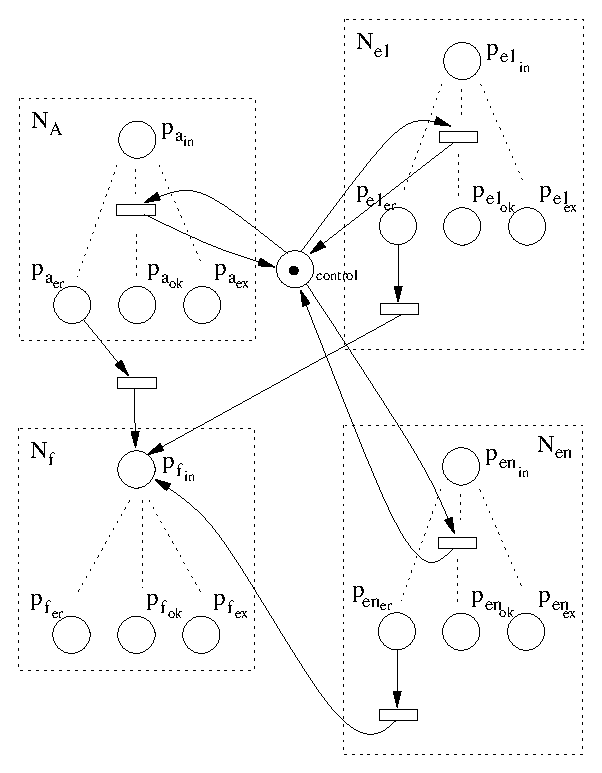
\includegraphics[scale=0.5]{Figures/orchestration.eps}
}}\end{center}
\vspace{-0.65cm}
\caption{Orchestration Translation}\label{orchestator}
\end{figure}

%where \mbox{$e \in \nat$} is a natural value reserved to 
%represent that the variable has not yet been assigned.
 
%\item {\em Activities}\,:\, The translation for each one is shown in
%the following subsections.
%\end{itemize}


{\it Variables and resources}: There is one place for each variable, whose token value is the current variable value. As regards resources, there are two places associated to each resource, $p_{\it r_i}$, $p_{\it r_a}$. For
any resource {\it r}, ${\it p_{r_a}}$ becomes marked when the orchestrator executes the \emph{createResource} activity, whereas the second one, ${\it p_{r_i}}$, is marked as far as the orchestrator does not execute the \emph{createResource} activity. When the resource lifetime terminates, the resource is released, passing the token from ${\it p_{r_a}}$ to ${\it p_{r_i}}$. Observe that we can know in advance the number of resources in the system by reading the WS-BPEL/WSRF document.

%After presenting the places that conform our timed net, we are going to analyse thoroughly the activities that constitute the process logic. We will start with the basic activities.

% ======================================================================
%                            BASICAS 
%=======================================================================

\subsection*{Basic activities}
\begin{itemize}
\item {\it Throw, Empty, Assign, Exit} and  {\it Wait} activities:\\
%
These are translated as indicated in \mbox{Fig.\ \ref{fig:basicas}},
by means of a single transition labelled
with the name of the corresponding activity linked with the corresponding terminating place. 
The time required  to execute 
{\it assign}, {\it empty}, {\it throw} and {\it exit} is negligible, so that the 
corresponding transitions have a null delay associated.
Notice that for the {\em assign} activity translation we use
a self loop between the transition and the
place associated with the variable ($p_{\it v}$)
in order to replace its previous value by the new one, being this new value obtained from an expression (exp) consisting of variables $p_{v1},\ldots,p_{vn}$ and integers. For the {\it wait}
activity, we have a time interval $[a,b]$ associated, so the delay is randomly selected
inside this interval. Notice the use of a ``control'' place, to arrest all possible remaining activities in the system when either throw or exit are executed. Thus, the idea is that all transitions in the net must be connected with this place, as the different illustrations show.
\begin{figure}[h]
\centering
\fbox{\parbox[h]{\textwidth}{
\subfigure[Throw PTCPN.\label{fig:throw}]{
    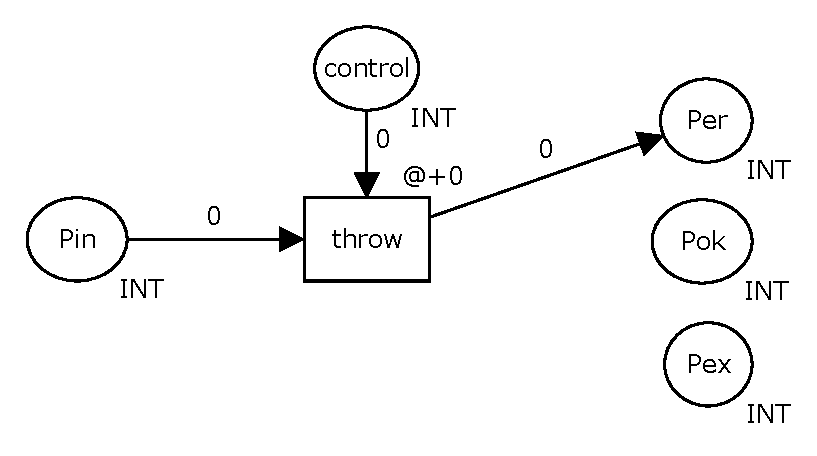
\includegraphics[scale=0.3]{Figures/throw.eps}
}
\hfill
\subfigure[Exit PTCPN.\label{fig:exit}]{
    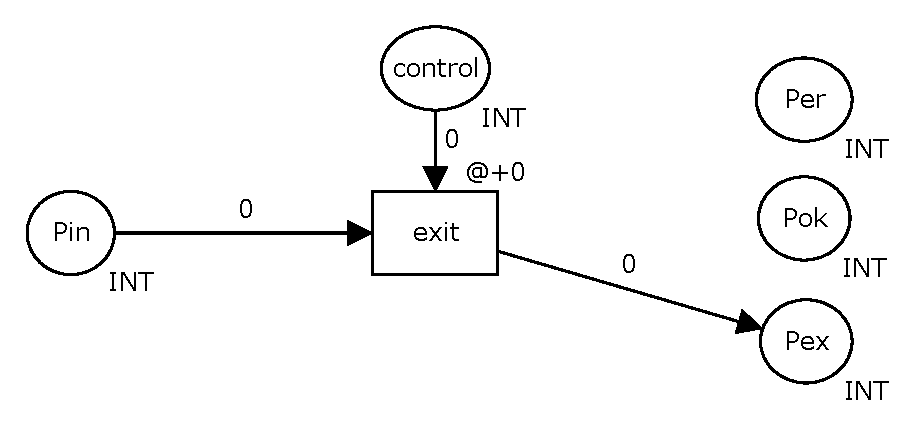
\includegraphics[scale=0.3]{Figures/exit.eps}
}
\hfill
\subfigure[Empty PTCPN.\label{fig:empty}]{
    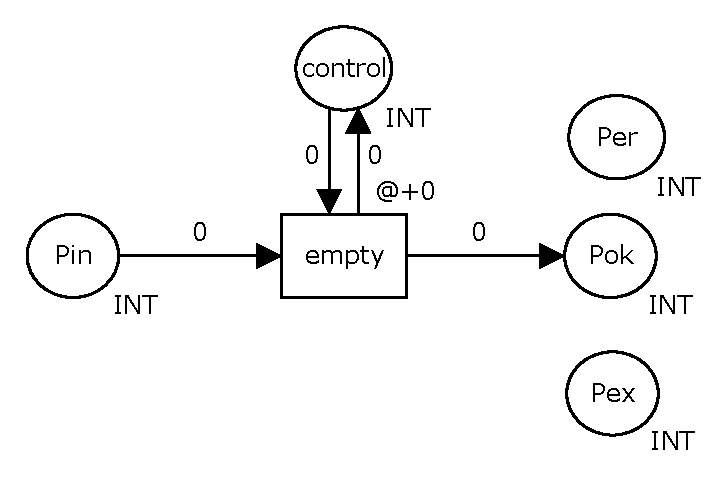
\includegraphics[scale=0.3]{Figures/empty.eps}
}
\vfill
\hspace{1cm}
\subfigure[Wait PTCPN. \label{fig:wait}]{
    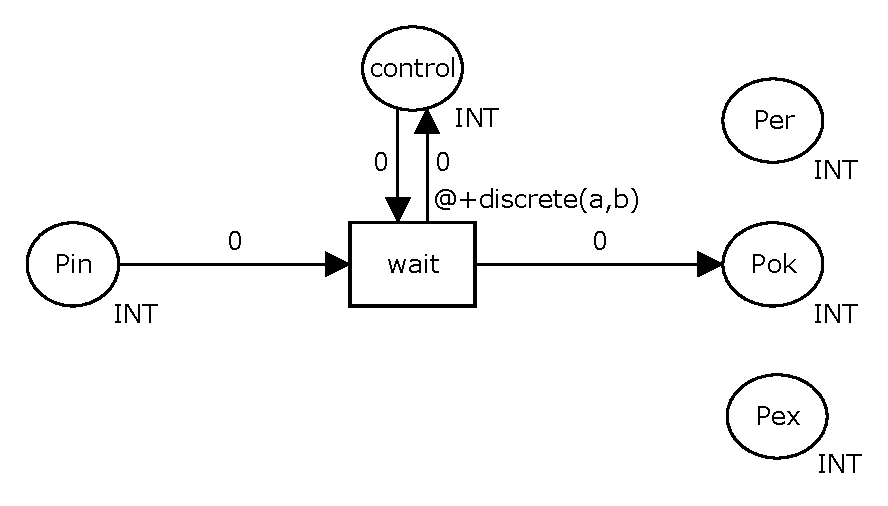
\includegraphics[scale=0.3]{Figures/wait.eps}
}
\hspace{1cm}
\subfigure[Assign PTCPN.\label{fig:assign}]{
   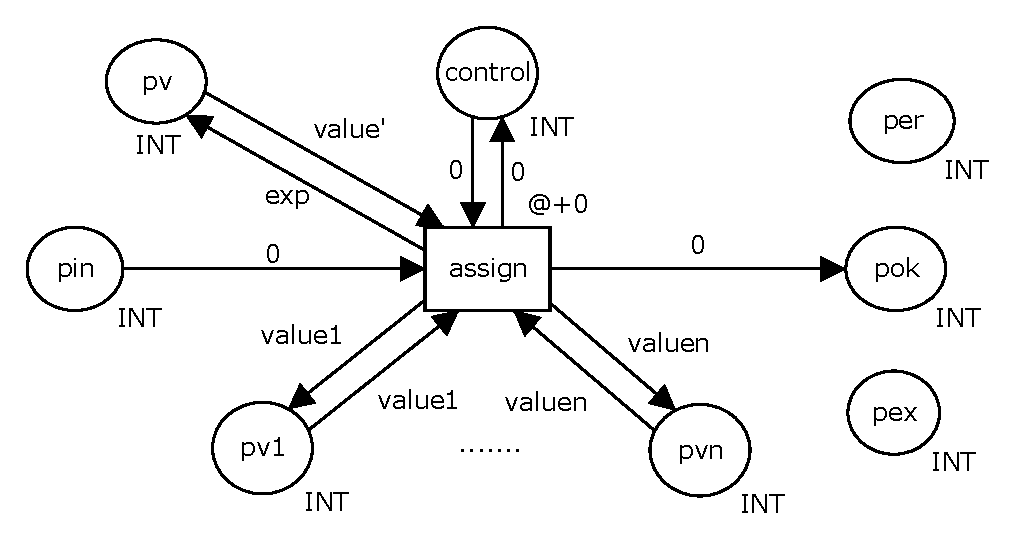
\includegraphics[scale=0.3]{Figures/assign.eps}
}
}}
\caption{\label{fig:basicas}Basic Activities
Translation}
\end{figure}

\item {\it Communication activities}:
The model we use is based on the invoke and receive operations, 
as well as the reply activity that uses a server to reply to a client. We have also added a barred version
of reply to synchronise with the response from the client. We have therefore introduced 
this last activity in our semantics to deal with the synchronous or asynchronous nature of invoke activity (one-way or request-response operation, respectively), so the $\overline{reply}$ activity is optional in the syntax depicted in Table \ref{BPELsyntax}. 

\begin{figure}[h]
\centering
\fbox{\parbox[h]{\textwidth}{
\subfigure[Invoke/Receive PTCPN.\label{fig:comm1}]{
    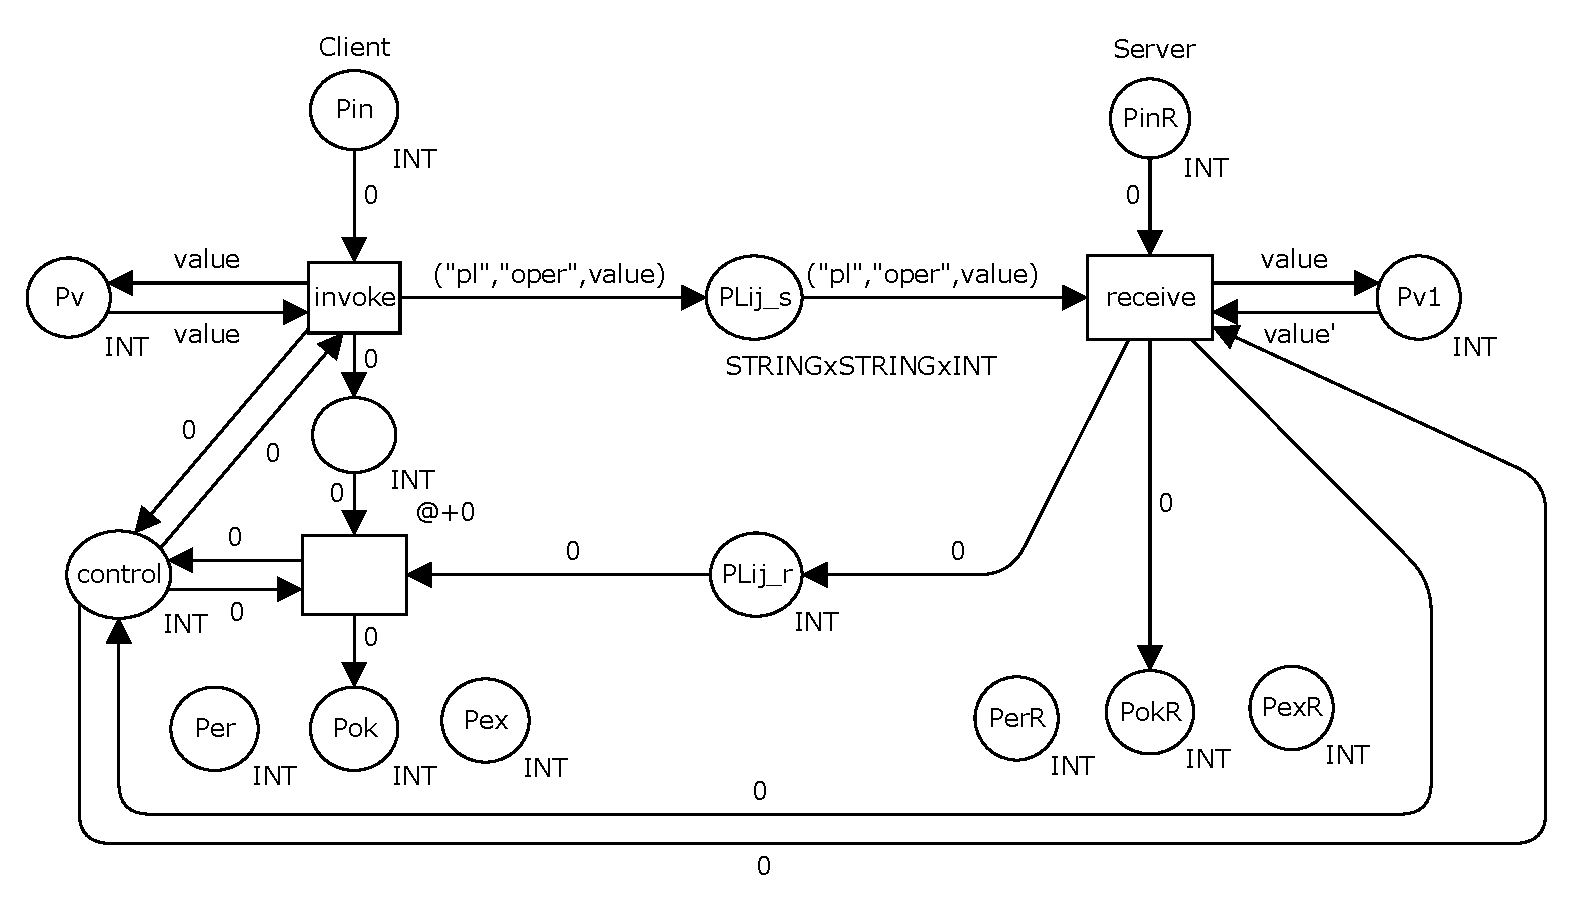
\includegraphics[scale=0.27]{Figures/communication.eps}
}
\hfill
\subfigure[$\overline{Reply}$/Reply PTCPN.\label{fig:comm2}]{
    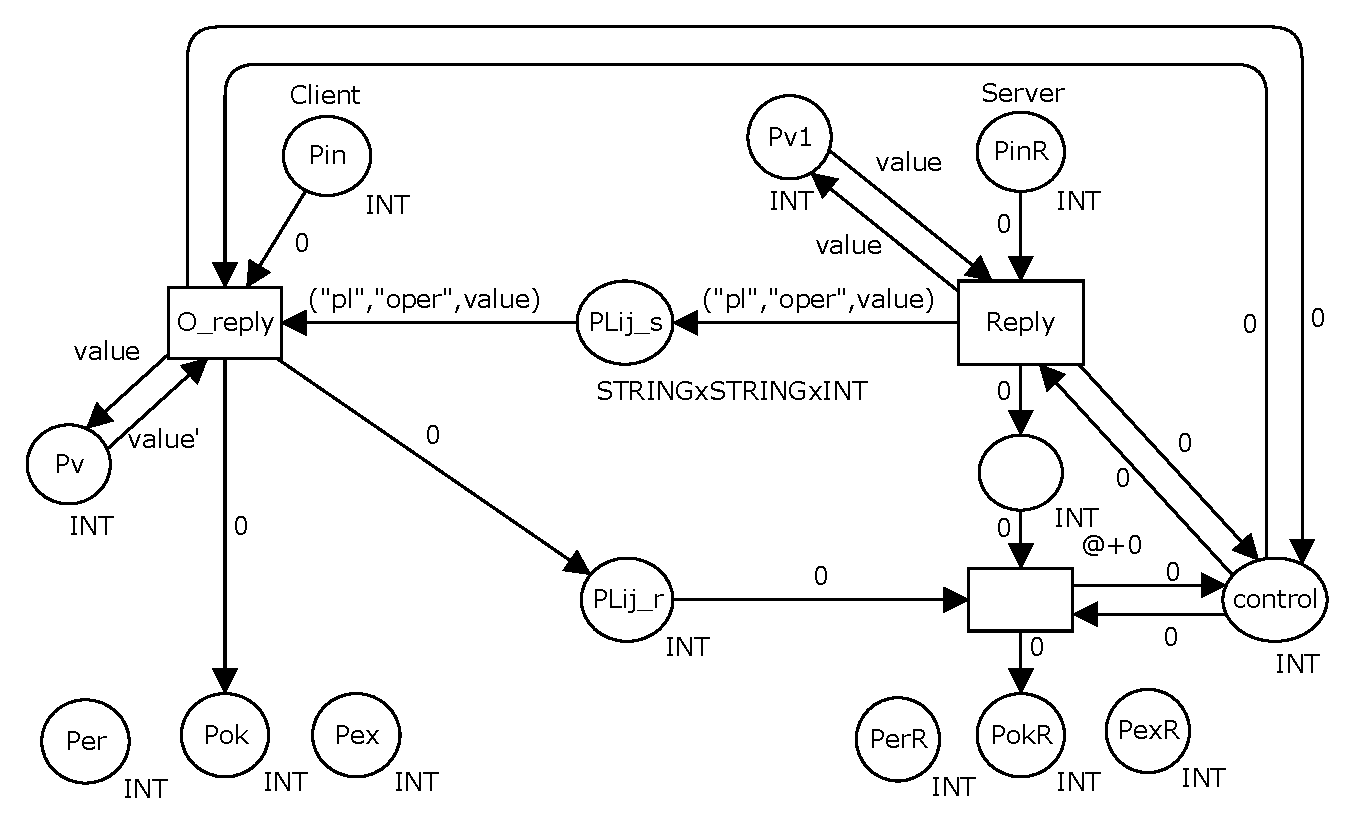
\includegraphics[scale=0.3]{Figures/communication_2.eps}
}
}}
\caption{\label{fig:comm}Invoke/Receive Activities
Translation} 
\end{figure}
%In this case, we have added to our timed Petri net two specific places in order to manage the execution of invoke/receive and reply/$\overline{reply}$, $PLij\_s$ and $PLij\_r$. Thus, we only require two places to represent all the partnerlinks between two services since we will bind each one with its corresponding counterpart by using the colours of the tokens. Place $PLij\_s$ receives tokens with three parameters: $pl,op$ and $value$, whereas $PLij\_r$ is marked only when the activity has received the data, so this place is marked with the value 0. For the sake of simplicity, we exchange only the value of the variables, but this could be easily extended to any kind of data. We depict the Petri nets in Fig. \ref{fig:comm} that express the communication among partners. In Fig. \ref{fig:comm1}, the \emph{invoke} activity extracts the value to send from the variable place ${\it P_v}$ and mark the ``sending'' partnerlink with a token endowed with this information. Once this place is marked, the receive transition can be fired marking $PLij\_r$ to allow the invoke activity to continue, and storing directly the data exchanged in the corresponding variable place. The interpretation of Fig. \ref{fig:comm2} is analogous.  
Fig.~\ref{fig:comm} shows the translation for both the invoke/receive and the reply/$\overline{reply}$ pairs of activities. Part a) of the figure corresponds to the invoke/receive translation, in which the net of the invoke activity is depicted on the left-hand-side part, whereas the receive activity is depicted on the right-hand-side part. There are two shared places, $PL_{ij{_s}}$ and $PL_{ij{_r}}$, which are used to implement the synchronisation between the invocation and reception of services. Both places are associated to the partnerlink used for this communication, denoted here by $(i,j)$, where $i$ and $j$ are the orchestrator identifiers performing those activities. Notice that the value of a single variable is transmitted, which is obtained from the corresponding variable place, $p_v$. In the same way, the receive activity stores this value in its own variable. The interpretation of Part b) Fig.~\ref{fig:comm} is analogous.  
\end{itemize}
%
% ======================================================================
%                            ORDERING 
%=======================================================================
\subsection*{Ordering structures}

%Structured activities prescribe the order in which a collection of activities is executed. They 
%describe how a business process is created; by composing the basic activities and the WSRF-compliant activities (presented previously)
%it performs into structures that express the control patterns, handling of 
%faults and external events, and coordination of message exchanges between process instances 
%involved in a business protocol.  
WS-BPEL defines structured activities for various control-flow patterns:
\begin{itemize} 
\item Sequential control between activities is provided by $<$sequence$>$, $<$if$>$, \linebreak $<$while$>$, 
$<$repeatUntil$>$, and the serial variant of $<$forEach$>$. 
\item Concurrency and synchronization between activities is provided by $<$flow$>$ and the 
parallel variant of $<$forEach$>$.  
\item Deferred choice controlled by external and internal events is provided by $<$pick$>$.  
\end{itemize}
The set of structured activities in WS-BPEL is not intended to be minimal \cite{Andrews2003WSBPEL}, so there are cases where 
the semantics of one activity can be represented using another activity. Nevertheless, in order to reduce the complexity
of our translation, our approach omits many derived activities only dealing with the most important ones from the modelling viewpoint,
such as sequence, parallel and choice. For all these cases we provide the translation
by only considering two activities. However, the generalization
to a greater number of activities is straightforward in all
of them. 
\begin{itemize}

\item {\it Sequence}\,: A sequence of two activities $A_1;A_2$ (with PTCPNs $N_{A_1}$ and
      $N_{A_2}$, respectively)
      is translated in a simple
      way (Fig.\,\ref{seq}), by just collapsing in a 
      single place (this will be
      an internal place of the new PTCPN)
      the {\it output} place ${\it Pok}$ of $N_{A_1}$, and the
      {\it entry} place of $N_{A_2}$.  The {\it entry} place
      of the new PTCPN will
      be the {\it entry} place of $N_{A_1}$. The
      {\it output} place of the new PTCPN will
      be the {\it output} place of  $N_{A_2}$, and we also
      collapse the {\it exit}, {\it error} and {\it control}  places of both PTCPNs.

%\vspace{1cm}

\begin{figure}[!ht]
\begin{center}
\fbox{\parbox[]{6cm}{\center
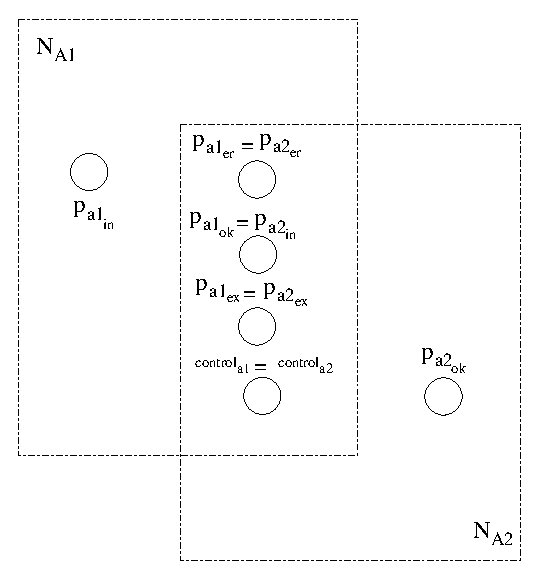
\includegraphics[scale=0.5]{Figures/sequence.eps}}}
\end{center}
\caption{\label{seq} Sequence Translation}
\end{figure}

\item {\it Parallel}\,: The translation for a parallel activity is depicted
in Fig.\,\ref{par}, which includes two new transitions $t1$ and
$t2$. The first to fork both parallel activities
and the second to join them when correctly terminated. 
Transition $t1$ thus puts one token on the initial places of both
PTCPNs, $N_{A_1}$ and $N_{A_2}$, in order to activate them,
and also puts one token on a new place, $p_c$, which is
used to stop the execution of one branch when the other has
failed or the exit activity is explicitly executed in one of them.
This place is therefore a precondition of every 
transition in both PTCPNs, and it is also a postcondition
of the non-failing transitions. However, in the event
of a failure or an exit activity, the corresponding {\em throw} or {\em exit}  transition
will not put the token back on $p_c$, thus
arresting the other parallel activity.

Notice also that the {\em error} places of ${N}_{A_{1}}$ and $N_{A_{2}}$
have been joined in a single error place ($p_{\it er}$),
which becomes marked with one token on
the firing of one {\em throw} transition. 
In this case, the other activity cannot execute any
more actions ($p_c$ is empty), so some dead tokens would
remain permanently on some places in the PTCPN.
However, these tokens cannot cause
any damage, since the control flow has been
transferred either to the fault handling activity of the PTCPN, 
once the place $p_{er}$ has become marked, or the whole system has terminated once 
the place $p_{ex}$ is marked. A similar reasoning is done with the {\em exit} places.
It is a must to remark we do not treat 
some BPEL flow construction attributes such as join conditions,
dead path elimination, etc., since there are out of the scope of the language BPELRF.

\begin{figure}[!ht]
\begin{center}
\fbox{\parbox[t]{12cm}
{\begin{center}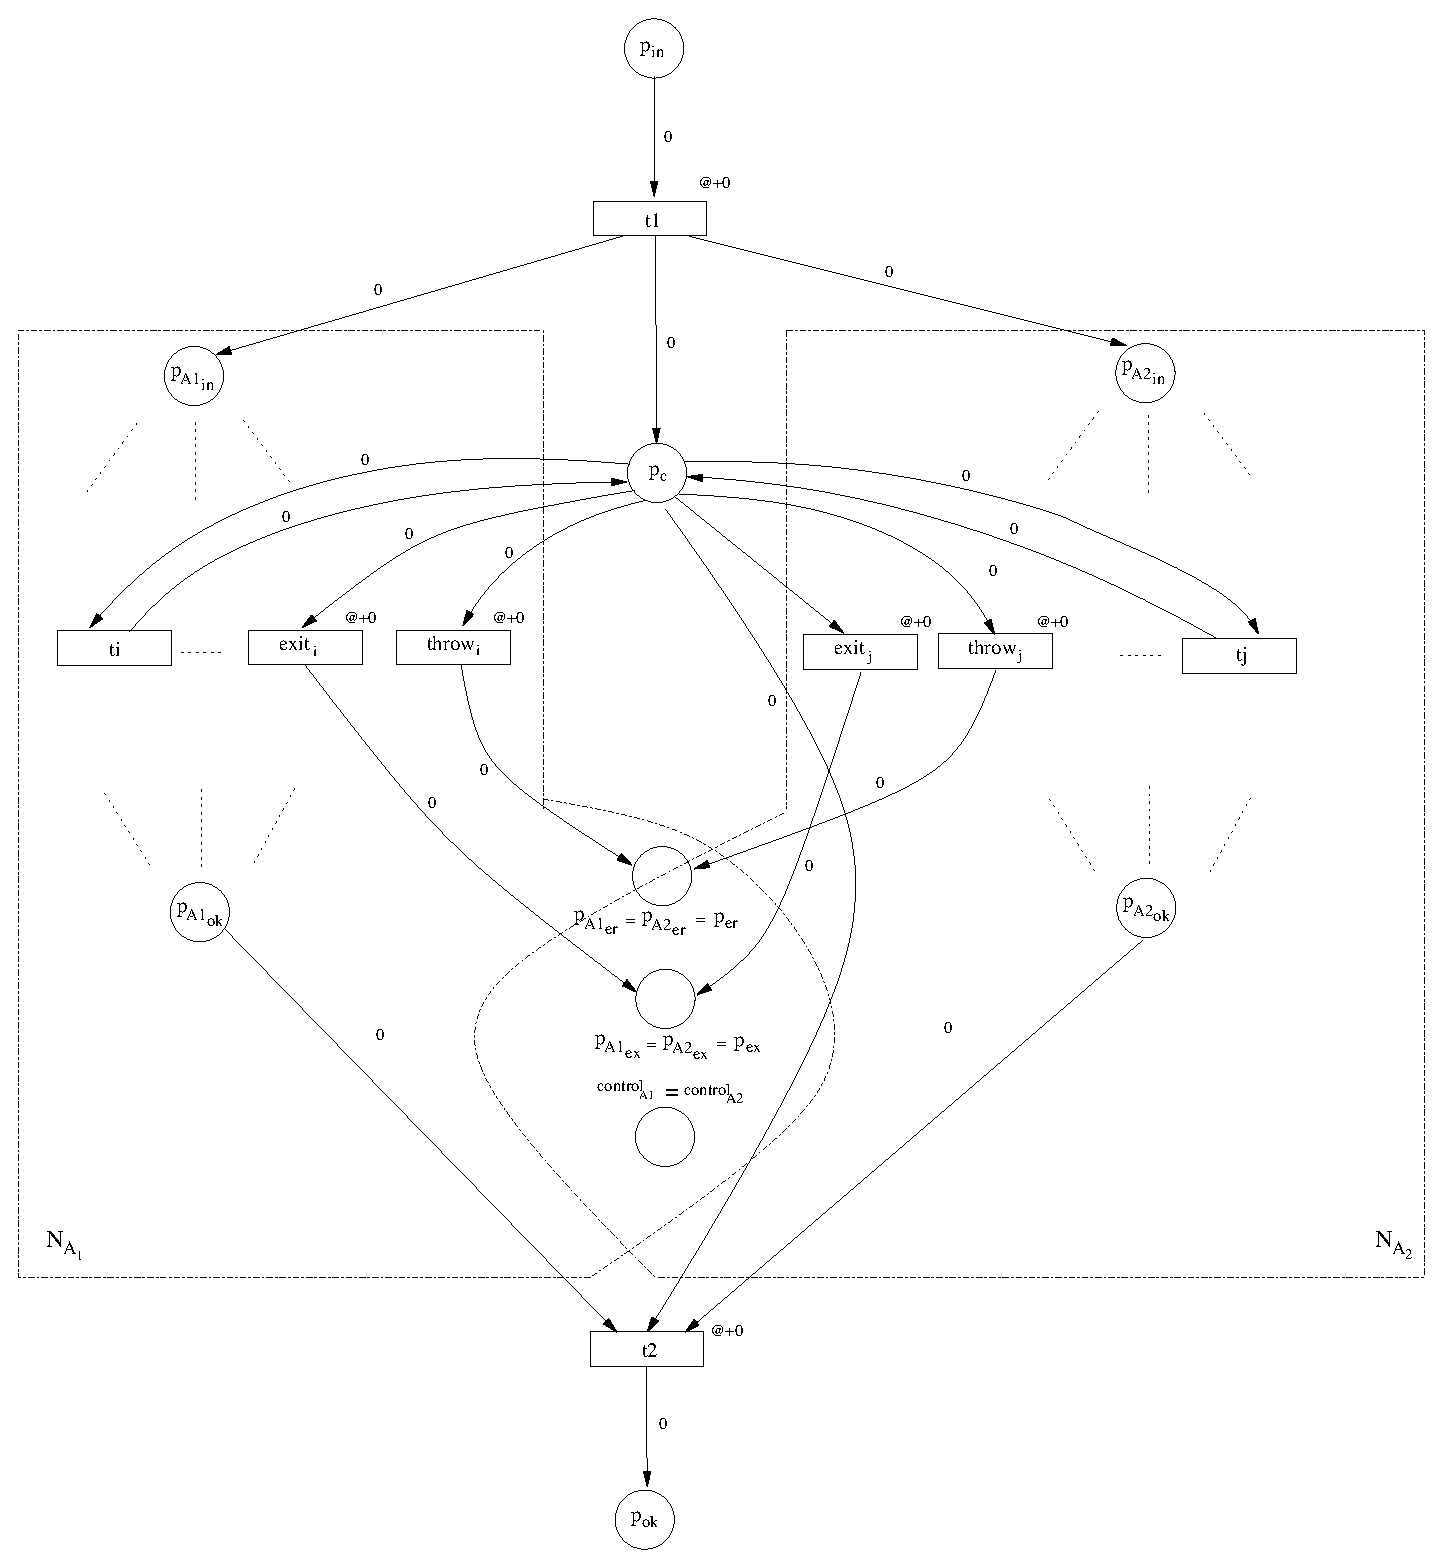
\includegraphics[height=10cm,width=12cm]
{Figures/paralelo.eps}\end{center}}}
\end{center}
\caption{\label{par} Parallel Activity Translation.}
\end{figure}

\item {\it Pick} $(\{(pl_i,op_i,v_i,A_i)\}_{i=1}^n,A,timeout)$: The $<$pick$>$ activity waits for the occurrence of exactly one event from a set of events, also establishing a
time-out for this selection. The translation is depicted in Fig.~\ref{pick} where a timer is implemented on the place {\it p\_a} in order to enforce the firing of transition {\it ta} when the timeout has elapsed, thus activating {\it N$_{A}$}. Notice also the use of both timed and untimed places in this figure, respectively called {\it INT} and {\it UINT}.  The $<$pick$>$ activity completes when the selected activity finishes, and, then, executes the activity associated with that event. After an event has been selected, the other events 
are no longer accepted by that $<$pick$>$. The $<$pick$>$ activity is comprised of a set of branches, each containing an event-activity pair.  
The activities contained in this construction can come in two forms: 

%\begin{itemize}
%\item The $<$onMessage$>$ is similar to a $<$receive$>$ activity, in that it waits for the receipt of an 
%inbound message. 
%\item The $<$onAlarm$>$ corresponds to a timer-based alarm. If the specified duration value 
%is zero or negative, or a specified deadline has already been reached or 
%passed, then the $<$onAlarm$>$ event activity is executed immediately. 
%\end{itemize} 
% must act in a similar fashion, but adding a feature
%which permits the selection among some activities. This selection is easy to model with Petri nets since collapsing the input places of the possible branches
%it is impossible to execute more than one at the same {\em pick}. In our model, the place {\em PinA1..An} represents this behaviour. Finally, in the BPEL specification, 
%is encouraged the use of time-outs with {\em pick} activity, so we have included a timed transition with its corresponding timed guard in order to manage the execution of 
%an ``alarm activity'' only in the event the time-out expires. The meaning of the other places and transitions is the same as in the receive activity.  
\begin{figure}[!ht]
%\vspace{-0.5cm}
\begin{center}
\fbox{\parbox[c]{12cm}{\begin{center}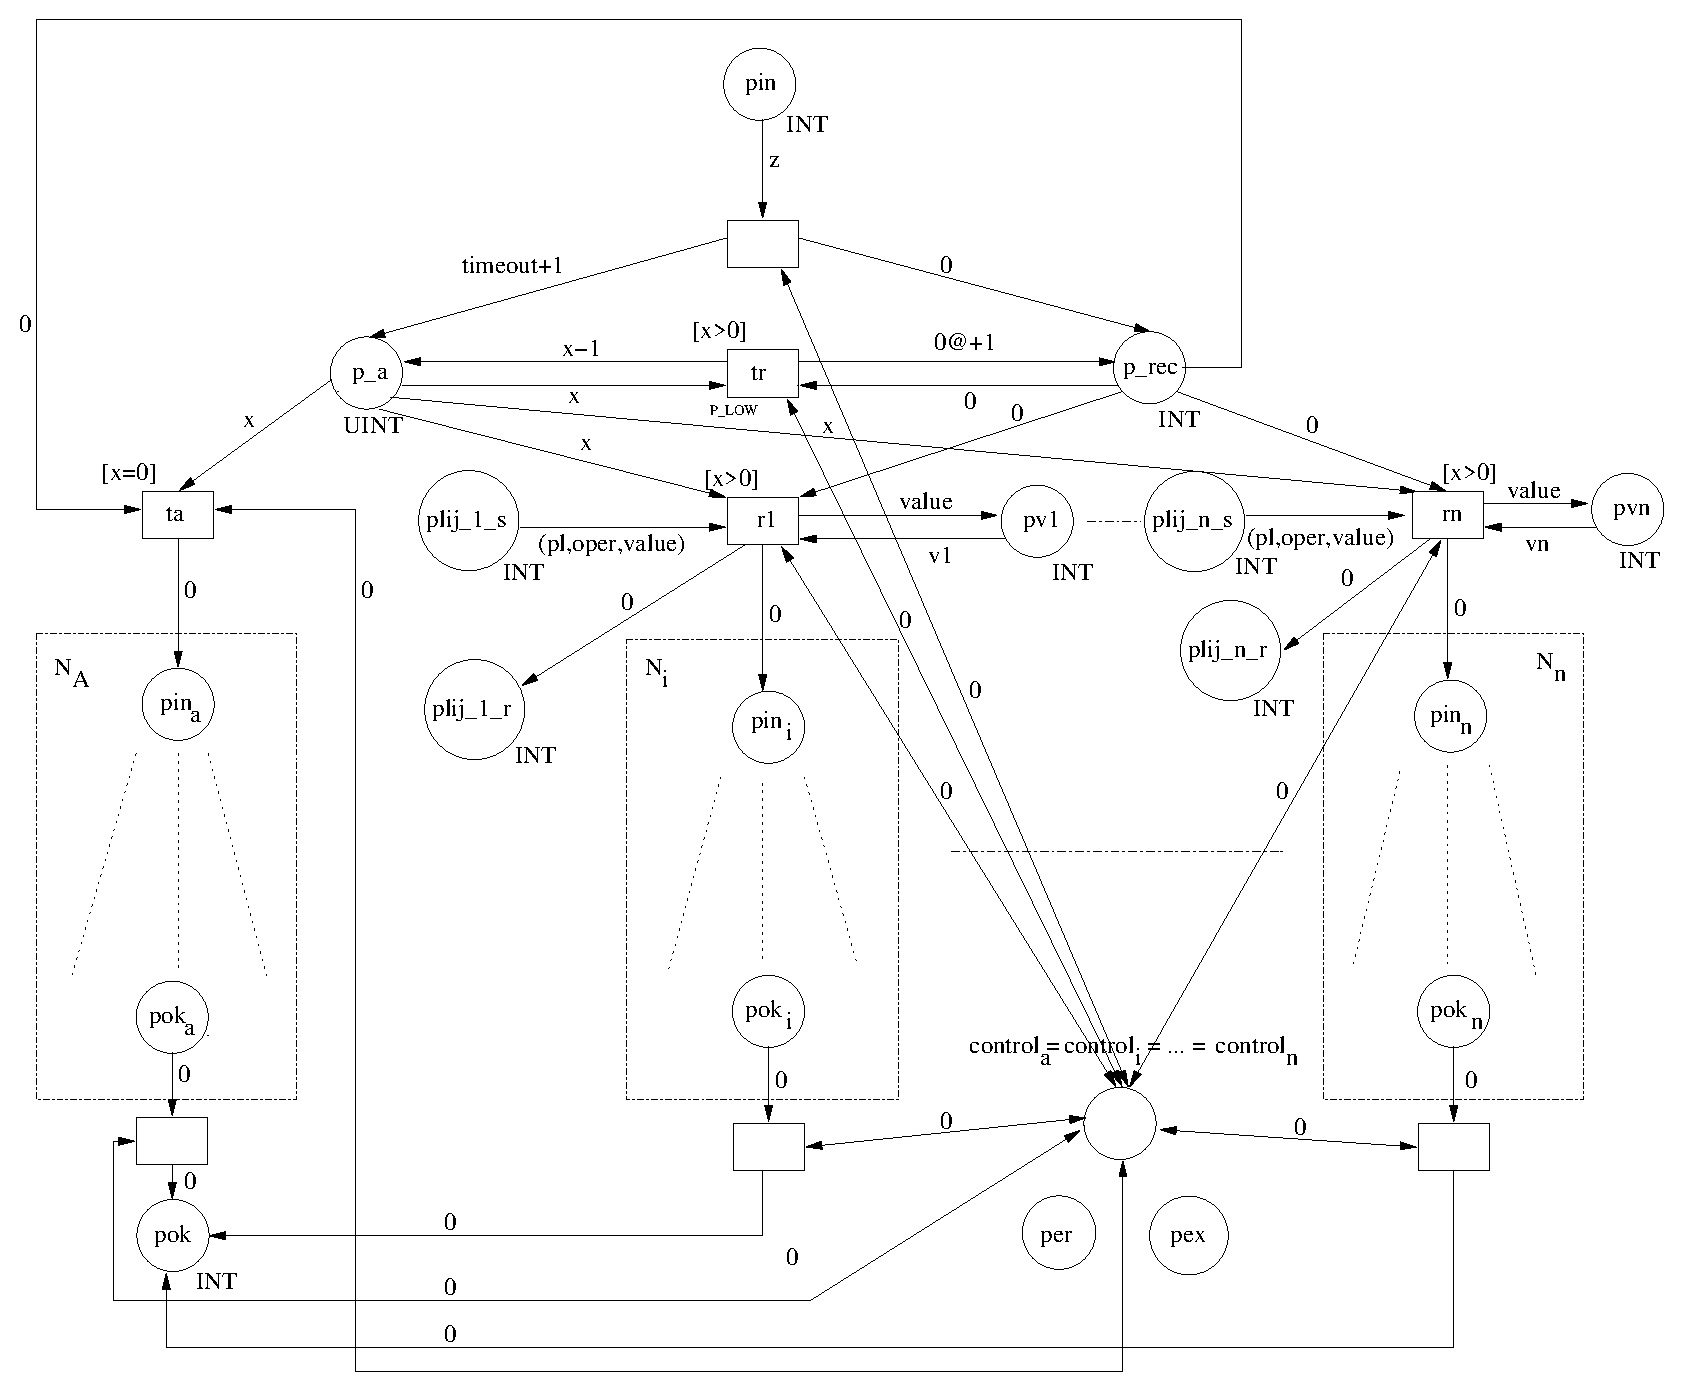
\includegraphics[scale=0.4]
{Figures/pick.eps}\end{center}}}
\end{center}
\caption{\label{pick} Pick Activity Translation.}
%\vspace{-0.4cm}
\end{figure}

\item {\it While} (cond,A): The machinery needed to model this construction is fairly straightforward since we only must check if the repetition condition holds or not in order to execute the contained activity or skip it. Fig.~\ref{while} shows this translation.
\end{itemize}
The $<$while$>$ activity provides for repeated execution of a contained activity. The contained 
activity is executed as long as the boolean condition evaluates to true at the beginning of 
each iteration. The meaning of the places and transitions of the net represented in Fig. \ref{while} is fairly straightforward, so, due to space limitations, we are going to omit any explanation of its elements. 
The meaning of the places and transitions are fairly straightforward, so, due to space limitations, we are going to omit any explanation of the elements contained in this net 

\begin{figure}[!ht]
%\vspace{-0.7cm}
\begin{center}
\fbox{\parbox[t]{11cm}{\begin{center}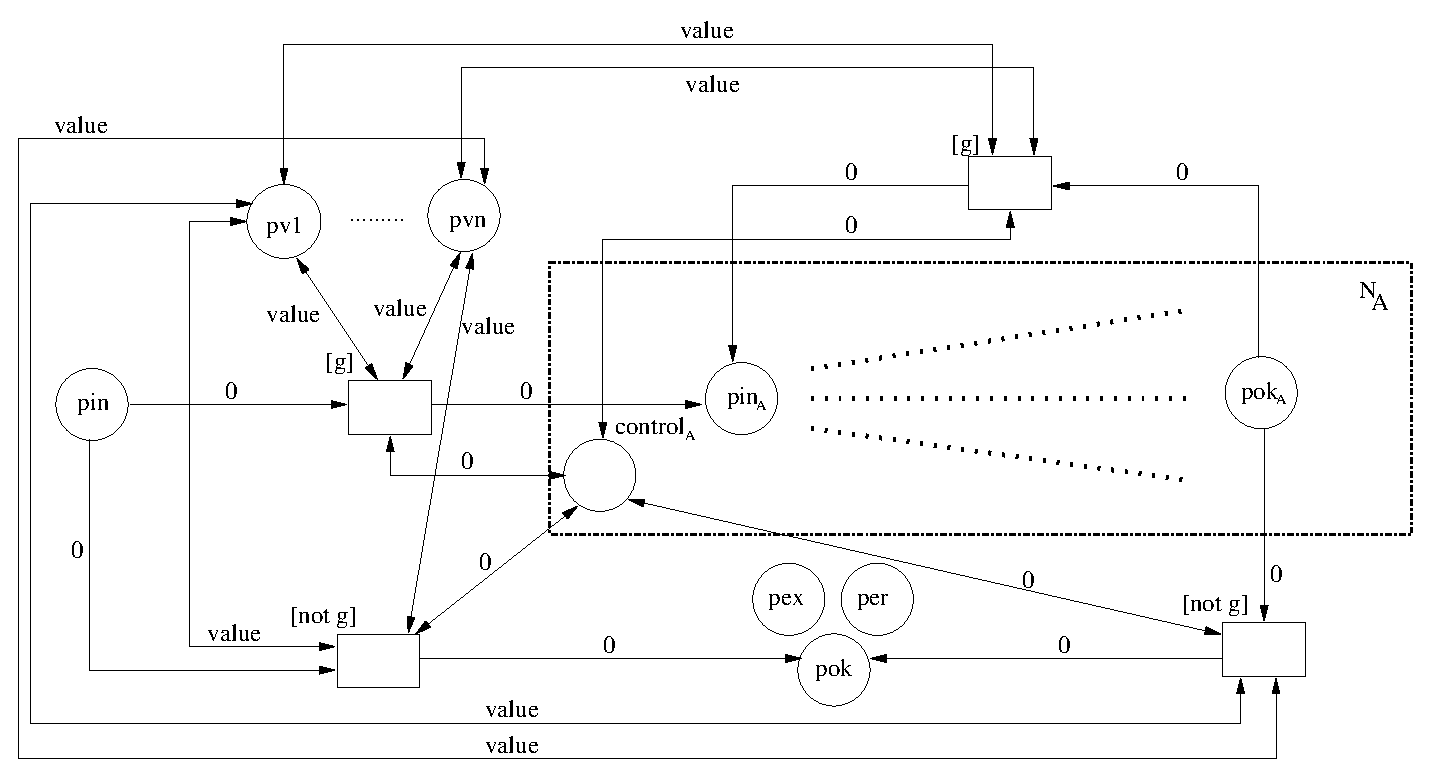
\includegraphics[scale=0.4]
{Figures/while.eps}\end{center}}}
\end{center}
\caption{\label{while} While Activity Translation.}
\vspace{-0.7cm}
\end{figure}
\vspace{-0.5cm}
\newpage
% ======================================================================
%                            WSRF 
%=======================================================================
\subsection*{WSRF/WSN-compliant}
In this section, we state the WSRF activities we have integrated with the BPEL activities in order to create a framework for modelling stateful workflows. 
%It is worth noting that in recent years have appeared a new redefinition of workflow nets which deals with resources called Resource-Constrained Workflow Nets \ref{}. As commented in the Related Work section, this approach extends the well-known formalism, Workflow nets, with finite resources such as money, memory and so on, but the authors do not provide the machinery
%to create and destroy such resources, so this extension of Workflow nets matches with the idea of WSRF standard, i.e., the creation and destruction of resources is out of the scope of the specification. Nevertheless, our approach was devised to manage the whole lifetime of the resource from its creation until its destruction.
To date, we have presented the activities corresponding to the \emph{BPEL part} of our model. Next, we will state the counterpart of our approach, i.e., the activities, which permit the creation and modification of the resources as well as the management of the subscriptions to them following the indications of the standard WSRF. Notice that a novelty in our model is the creation of resources since WSRF does not specify how this creation is done.
%\begin{figure}[!ht]
%\vspace{-0.5cm}
%\begin{center}
%\fbox{\parbox[t]{12cm}{\begin{center}\includegraphics[scale=0.35]
%{Images/createResource.eps}\end{center}}}
%\end{center}
%\vspace{-0.7cm}
%\caption{\label{createresource} CreateResource Activity Translation.}
%\vspace{-1.5cm}
%\end{figure}

To begin with, we depict the creation of resources in Fig. \ref{createresource}. In order to guarantee our PTCPNs are 1-safe, we opted as commented above to model each resource with two dedicated places,  $p_{\it r_i}$, and $p_{\it r_a}$, which represent the possible state of the resources, instantiated or not instantiated, respectively. Thus, when an orchestrator wants to create a resource, the firing of the transition {\it createResource} moves the token from the ``inactive'' ($p_{\it r_i}$) to the ``active'' place ($p_{\it r_a}$) making available this resource to the subscribers. Once the place $p_{\it r_a}$ is marked and an orchestrator executes the activity {\em subscribe}, our translation can automatically build the subscriptions nets. 

Here, a subscription net is formed by a transition, whose guard is the subscription condition, and the subnet which corresponds to the translation of the activity that the subscriber wants to be executed just in case the subscription condition ${\it gc_i}$ holds. Notice that WSRF allows the creation of multiple subscriptions to the same resources by the same orchestrator, so we will allow this restriction. Despite the {\em subscribe} construction will be presented later, just comment here we have endowed each resource with a list that represents its subscribers with their {\em id} and an integer, $0$ or $1$, to denote whether the orchestrator with identifier {\em id} is subscribed or not. Finally, in the leftmost part of Fig. \ref{createresource}, we depict the net that will be fired in the event of the resource lifetime expires. In this situation, we return the token from the active place to the inactive place and immediately execute the activity {\em $Activity_timeisup$}, which will be passed as an argument of the {\em createResource} activity. This argument is not included in the WSRF specification, but we have incorporated it to show the benefits of the integration of both standards.       

%Now, we describe the PTCPNs who corresponds to the manipulation of resource value and lifetime as well the subscription to a specific resource. On the left side of Fig. \ref{fig:getproperty},
%the PTCPN for the activity {\em getProperty} is depicted. Here, the resource {\em value} obtained from $p_{\it r_a}$ is stored in the place of the corresponding variable. The reasoning done in the construction of the PTCPNs for the activities {\em setProperty} and {\em setTimeout} in Fig. \ref{fig:setproperty} is quite similar, but updating the resource value or its lifetime, respectively. Important to note that if an orchestrator is trying to access to a resource not instantiated, the fault place  $p_{\it er}$ will be marked starting the execution of the fault activity. 
%\begin{figure}[!ht]
%\vspace{-0.5cm}
%\hspace*{1.0cm}
%\begin{center}
%\fbox{ \parbox[t]{12cm}{ \center
%  \subfloat[GetProperty and Subscribe Activities]{\label{fig:getproperty}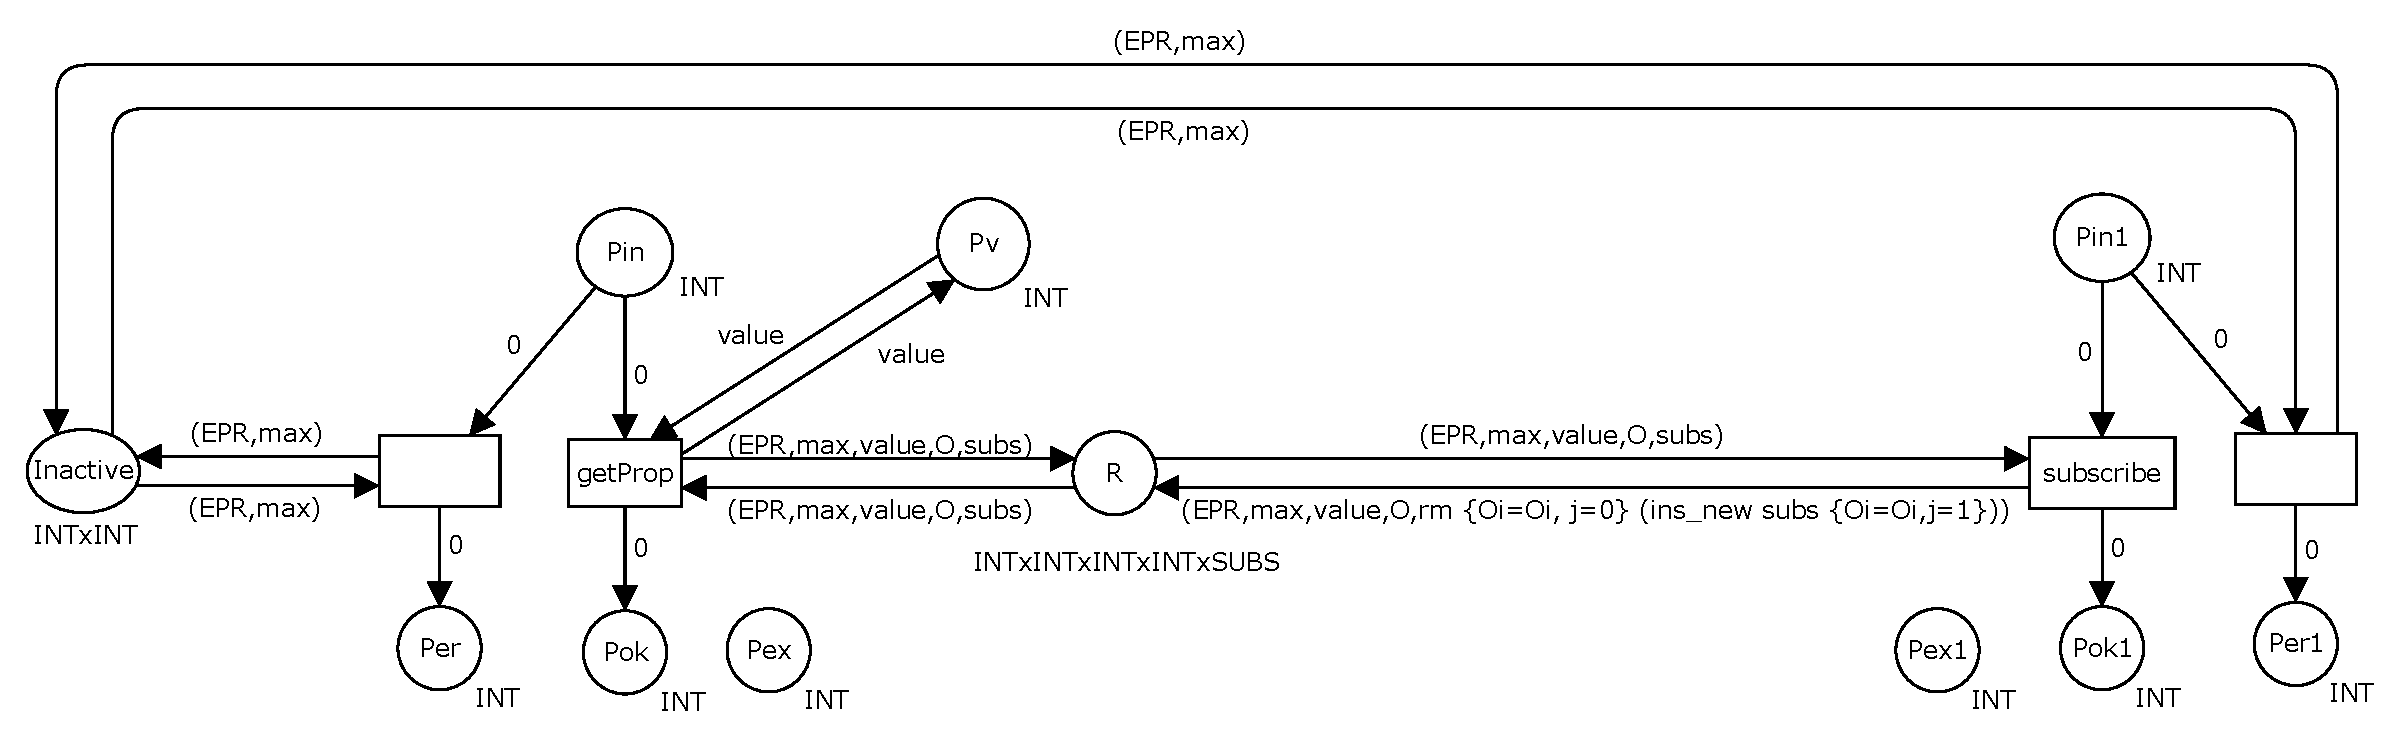
\includegraphics[scale=0.3]{Images/getProp+subscribe.eps}}\\
 % \subfloat[SetProperty and SetTimeout Activities]{\label{fig:setproperty}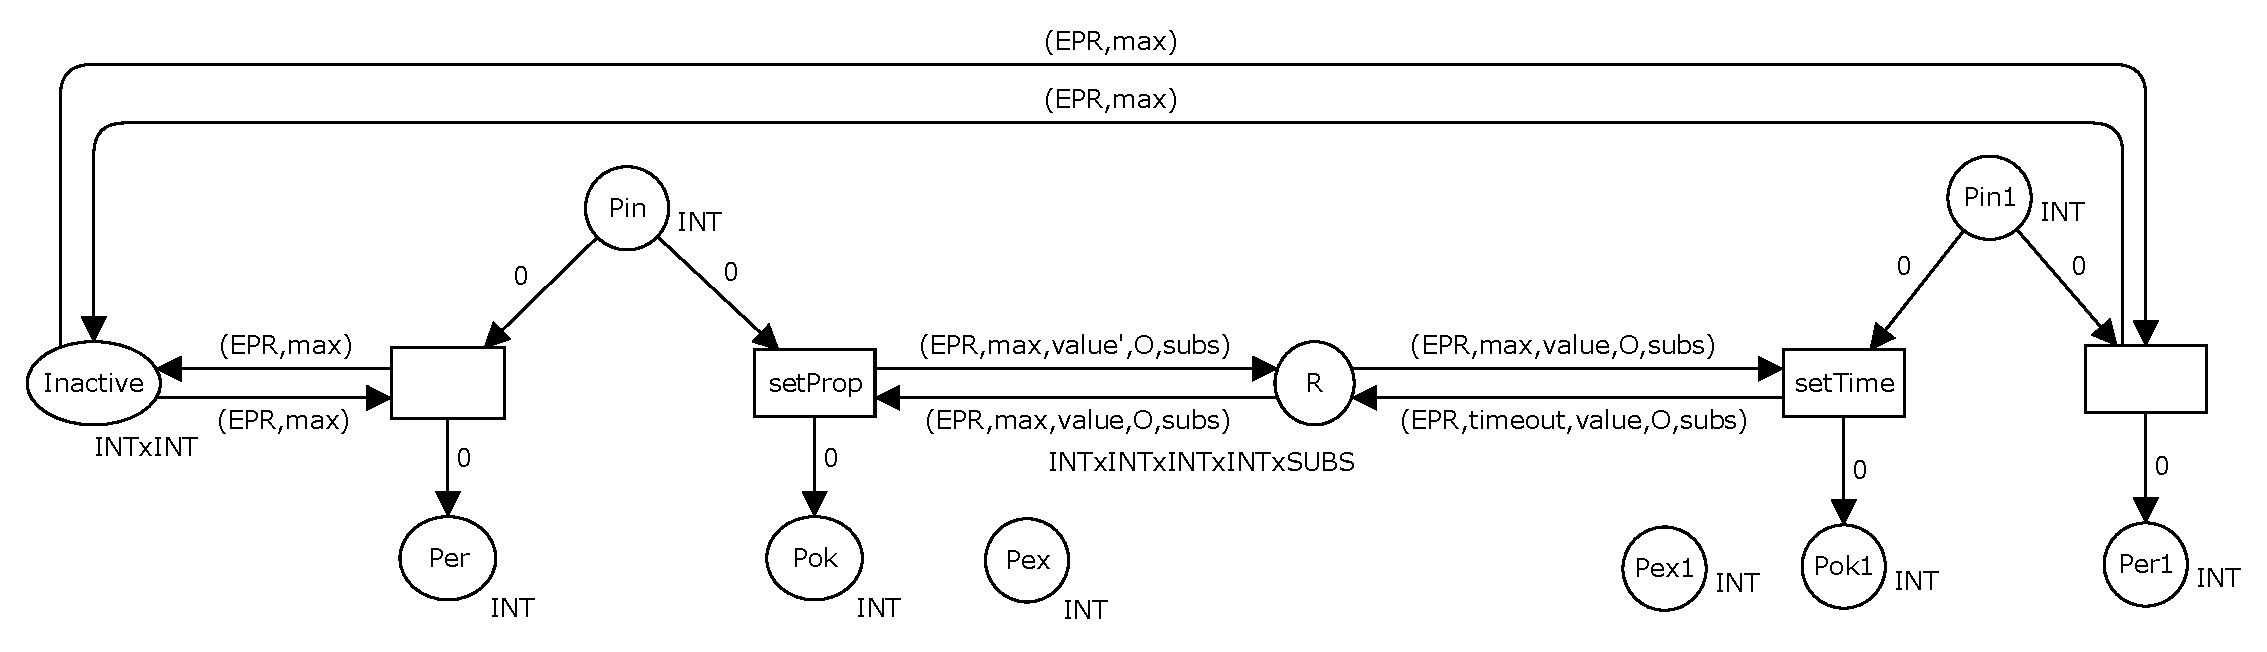
\includegraphics[scale=0.32]{Images/setProp+setTime.eps}}
 % }}
%\end{center}
%\vspace{-0.6cm}
%\caption{\label{fig_wsrf}WSRF Activities
%Translation}
%\vspace{-0.5cm}
%\end{figure}

%Finally, on the right side of Fig. \ref{fig:getproperty}, we show the PTCPN for the {\em subscribe} activity. Above, we have commented we have used a list to represent the subscribers of a resource. Since we have used CPNtools to build our nets, this ``registration stamp'' is modeled by using the record colour set provided by this tool. This record contains the identifier of the subscriber, {\em ID}, and integer variable {\em j}, whose value will be $0$ when the orchestrator is not subscribed and $1$ in the opposite case. This value will be checked in the guard of the first transition of the subscription net within the condition specified here in order to check if the orchestrator is subscribed and the condition holds. As in the previous cases, we run the fault activity if one orchestrator is trying to subscribe to non-instantiated resource.   

%\begin{figure}[!ht]
%\begin{center}
%\fbox{\parbox[t]{12cm}{\begin{center}\includegraphics[scale=0.35]
%{Images/setProp.eps}\end{center}}}
%\end{center}
%\vspace{-0.7cm}
%\caption{\label{setp} GetProperty Activity Translation.}
%\end{figure}

%\begin{figure}[!ht]
%\begin{center}
%\fbox{\parbox[t]{12cm}{\begin{center}\includegraphics[scale=0.35]
%{Images/getProp.eps}\end{center}}}
%\end{center}
%\vspace{-0.7cm}
%\caption{\label{setp} SetProperty Activity Translation.}
%\end{figure}

%\begin{figure}[!ht]
%\begin{center}
%\fbox{\parbox[t]{12cm}{\begin{center}\includegraphics[scale=0.35]
%{Images/setTime.eps}\end{center}}}
%\end{center}
%\vspace{-0.7cm}
%\caption{\label{settim} SetTimeout Activity Translation.}
%\end{figure}
\begin{itemize}
\item {\bf {\it CreateResource(EPR,val,timeout,A)}}:
{\em EPR} is the resource identifier, for which we have two complementary places in Fig.~\ref{createresource}, ${\it p_{r_i}}$ and ${\it p_{r_a}}$, where the sub-index represents the state of the resource: $i$ when it is inactive and $a$ when it is active. The initial value is $val$, and $A$ is the activity that must be executed when the time-out indicated as third parameter has elapsed.

We can see in Fig.~\ref{createresource} how the transition $createResource$ removes the token from the {\em inactive} place, and puts a new token on the active place, whose colour contains the following information: resource identifier (EPR), its lifetime (max), and its value (val). %the owner (O) and the list of subscribers (initially, empty).

\begin{figure}[!ht]
\begin{center}
\fbox{\parbox[t]{12cm}{\begin{center}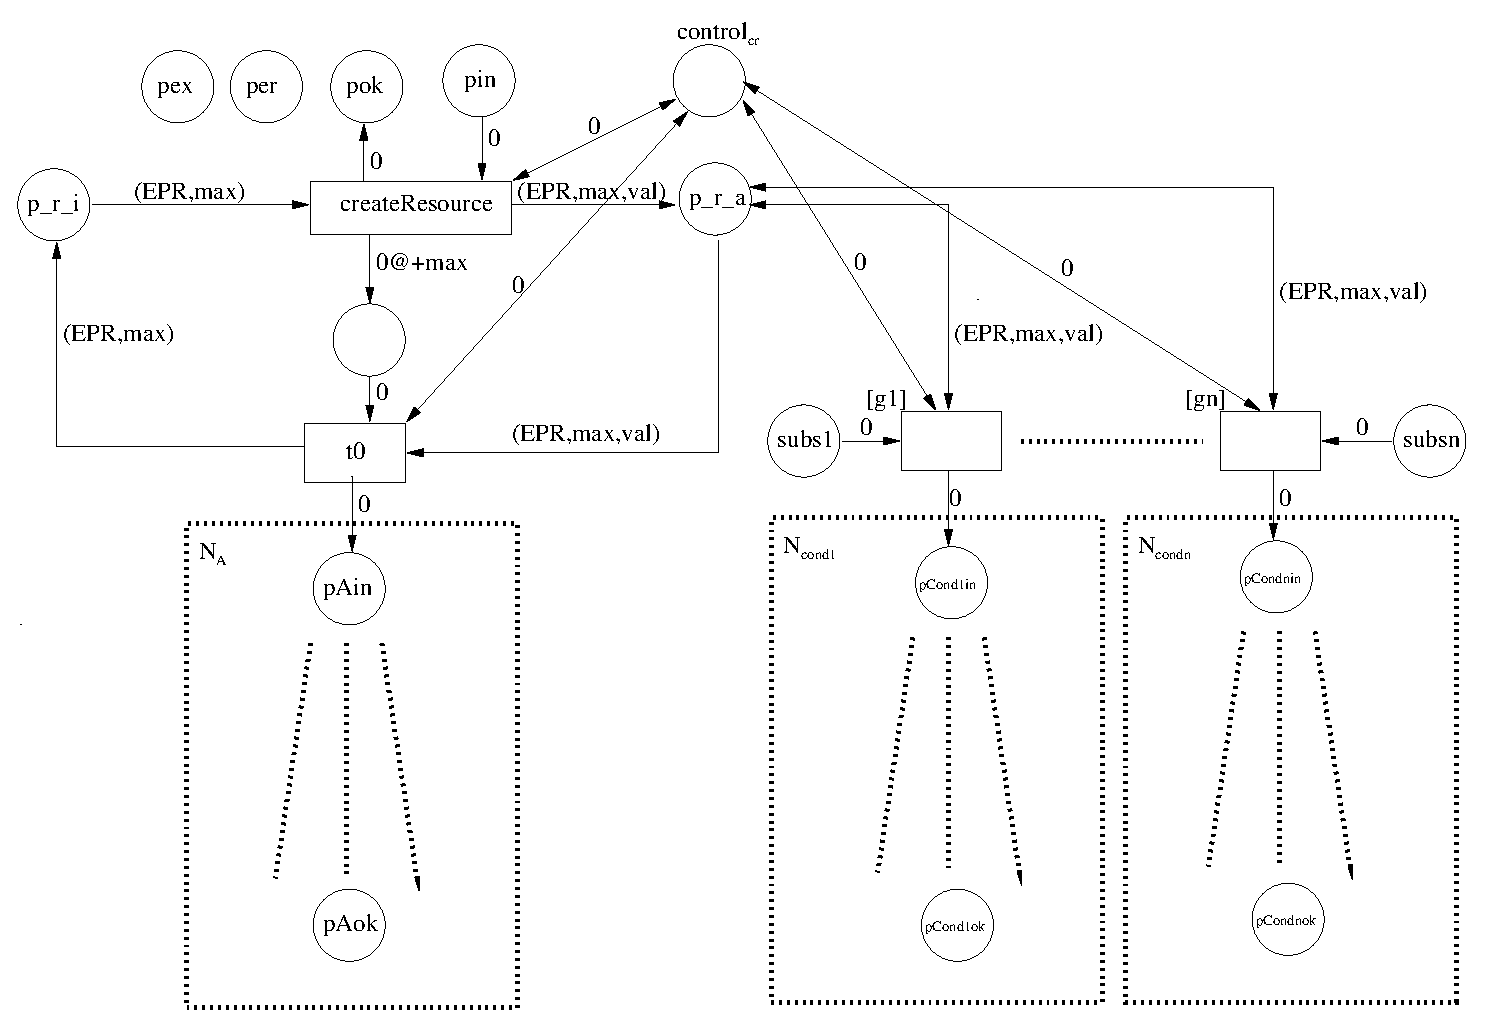
\includegraphics[scale=0.35]
{Figures/createResource.eps}\end{center}}}
\end{center}
\caption{\label{createresource} CreateResource Activity Translation.}
\end{figure}

Transition ${\it t}$0 is executed when the lifetime of the resource has expired, thus removing the token from the {\em active} place, marking again the {\em inactive} place, and activating $N_A$. We can also see that the {\em active} place is linked with a number of transitions, which correspond to the subscribers (we know in advance these possible subscribers from the WS-BPEL/WSRF document). These transitions can only become enabled if the corresponding places $subs_{i}$ are marked by performing the corresponding  activity {\em subscribe}. The PTCPNs ${\it Ncond_i}$ are the nets for the activities passed as parameter in the invocation of a subscribe activity.   

\item Subscribe (EPR,cond$'$,A):
In this case, an orchestrator subscribes to the resource $EPR$, with the associated condition $cond'$, upon which the activity $A$ must be performed. Fig.~\ref{subscribe} shows this translation, where we can observe that the associated place $subs_{i}$ is marked in order to allow the execution of the PTCPN for the activity $A$ if the condition $g_{i}$ holds. On the contrary, if the resource is not active, we will throw the fault handling activity.

%\begin{figure}[!ht]
%\vspace{-0.5cm}
%\hspace*{1.0cm}
%\begin{center}
%\fbox{ \parbox[t]{12cm}{ \center
%  \subfloat[GetProperty and Subscribe Activities]{\label{fig:getproperty}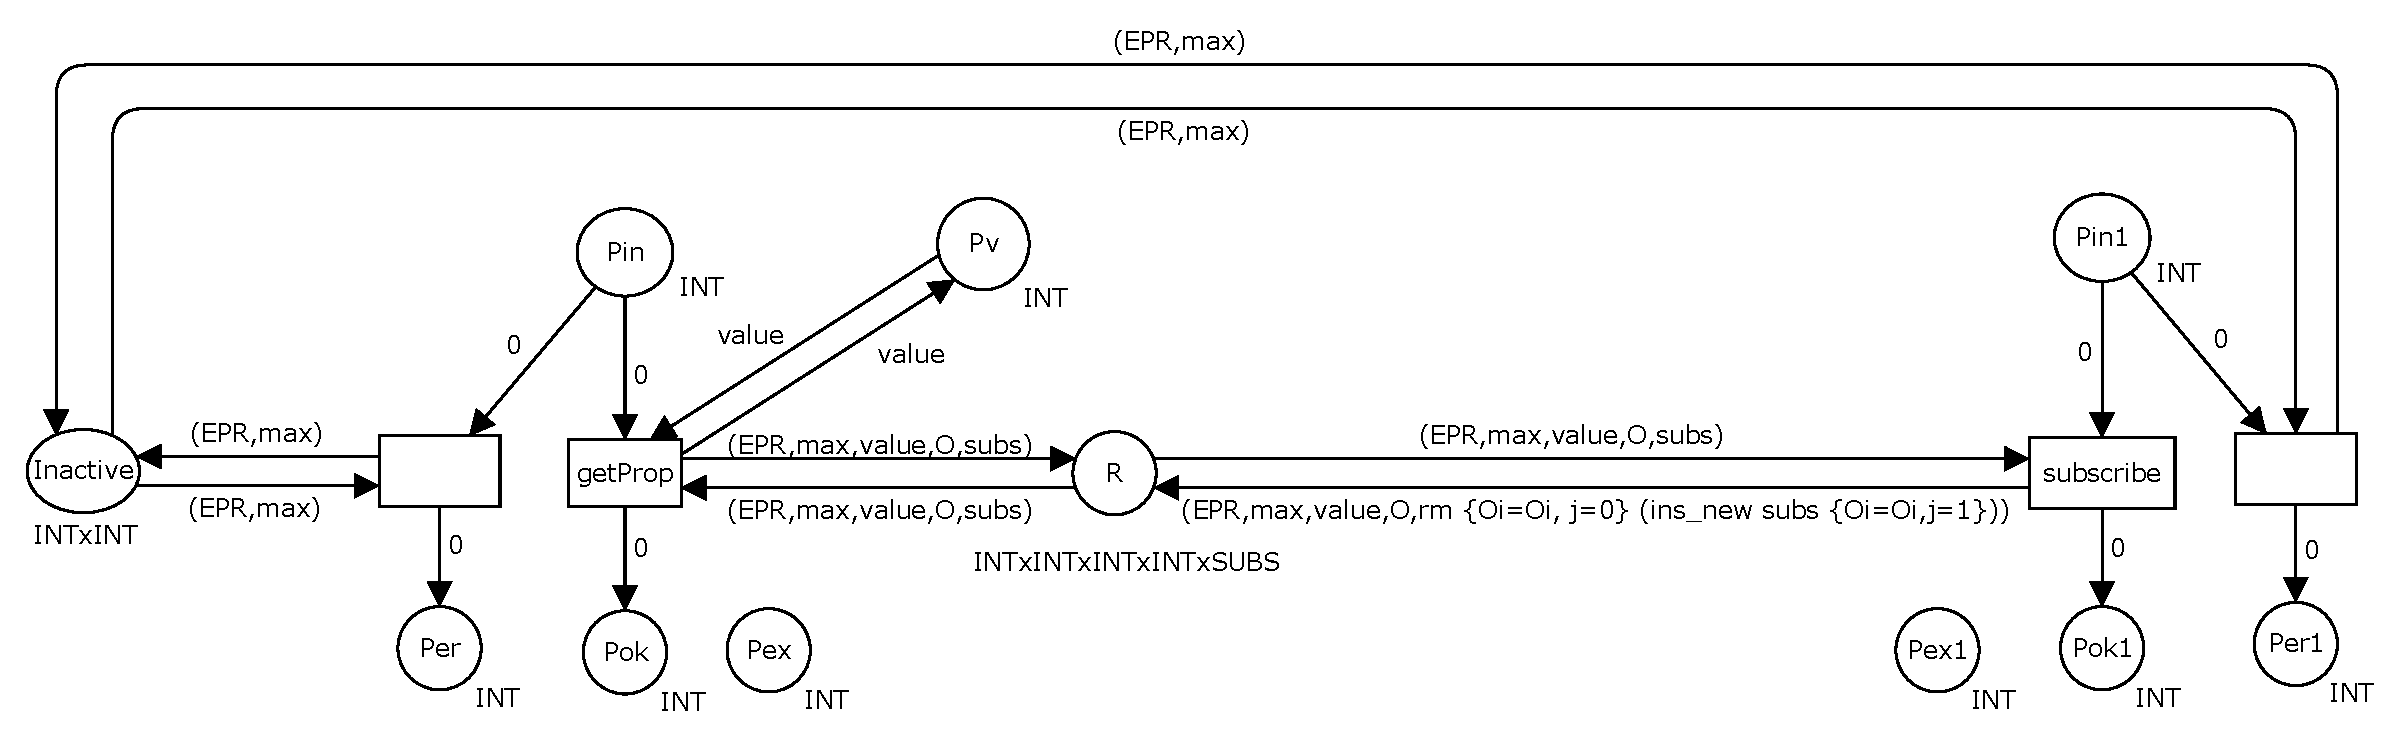
\includegraphics[scale=0.3]{Images/getProp+subscribe.eps}}\\
 % \subfloat[SetProperty and SetTimeout Activities]{\label{fig:setproperty}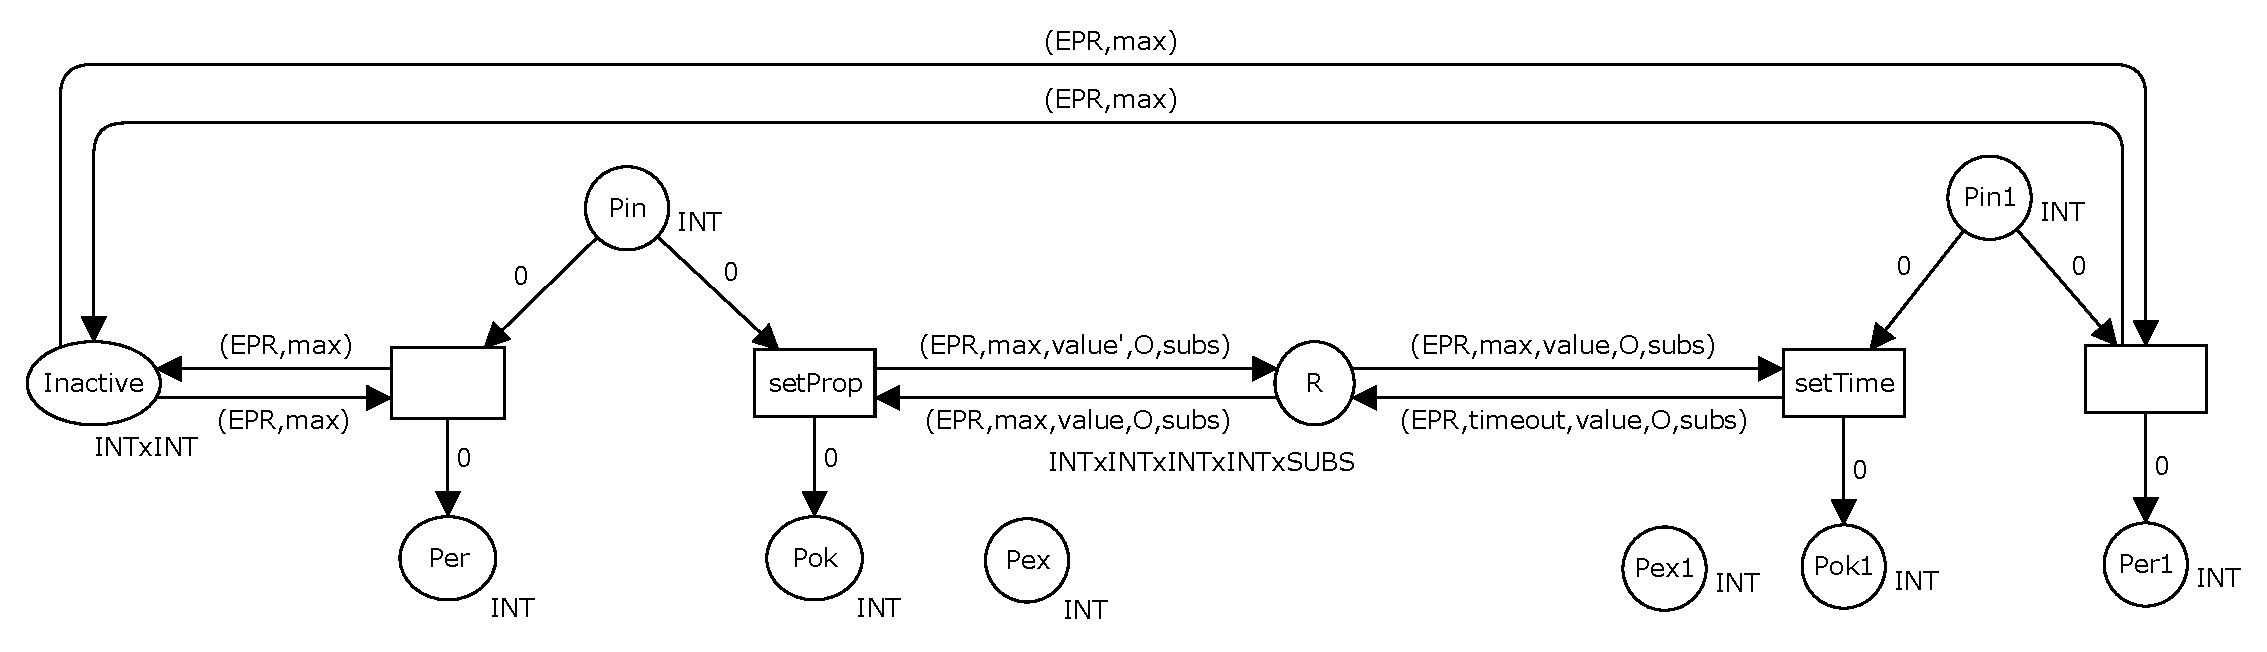
\includegraphics[scale=0.32]{Images/setProp+setTime.eps}}
 % }}
%\end{center}
%\vspace{-0.6cm}
%\caption{\label{fig_wsrf}WSRF Activities
%Translation}
%\vspace{-0.5cm}
%\end{figure}
\begin{figure}[!ht]
\begin{center}
\fbox{\parbox[t]{10cm}{\begin{center}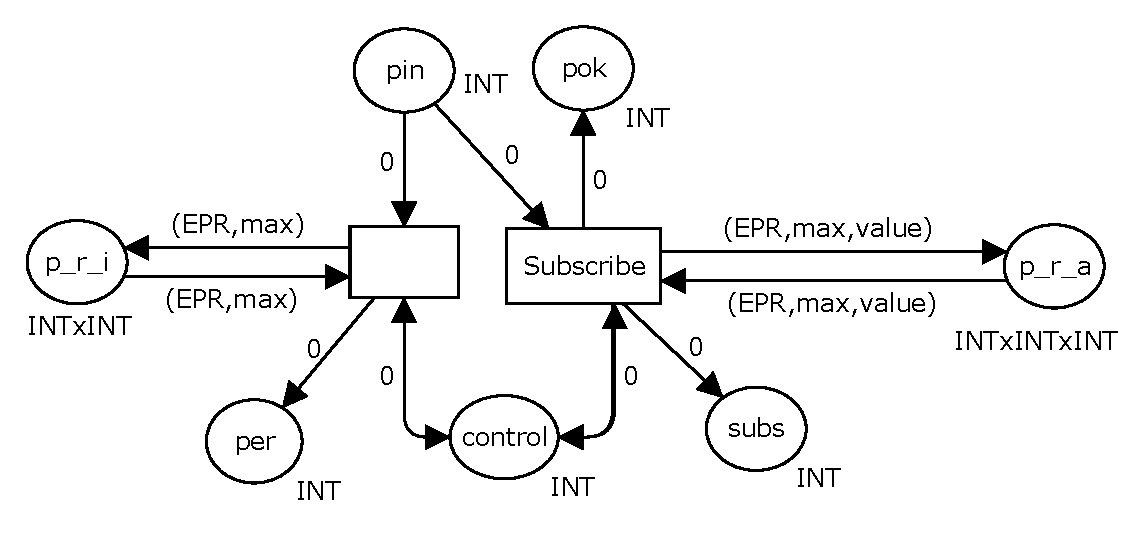
\includegraphics[scale=0.35]
{Figures/subscribe.eps}\end{center}}}
\end{center}
\caption{\label{subscribe} Subscribe Activity Translation.}
\end{figure}

\vspace{-0.4cm}

\item {\bf {\it GetProp (EPR,v)}} and {\bf {\it SetProp (EPR,expr)}}:
These are easily translated, as shown in Figs.~\ref{getp} and \ref{setp}, where the resource value is obtained and assigned to variable $v$ (GetProp), or a new value is assigned to the resource (SetProp).


\begin{figure}[!ht]
\begin{center}
\fbox{\parbox[t]{8.5cm}{\begin{center}\includegraphics[scale=0.35]
{Figures/getProp.eps}\end{center}}}
\end{center}
\caption{\label{getp} GetProperty Activity Translation.}
\end{figure}

%\begin{figure}[!ht]
%\vspace{-0.5cm}
%\hspace*{1.0cm}
%\begin{center}
%\fbox{ \parbox[t]{11cm}{ %\center 
%\hspace{-0.2cm}\subfloat[GetProperty Activity %Translation.]{\label{fig:get}\includegraphics[scale=0.4]{Images/getProp.eps}}\\
%\subfloat[SetProperty Activity %Translation]{\label{fig:set}\includegraphics[scale=0.4]{Images/setProp.eps}}\\
%\subfloat[SetTimeout Activity %Translation]{\label{fig:settime}\includegraphics[scale=0.4]{Images/setTime.eps}}
%}}
%\end{center}
%\vspace{-0.62cm}
%\caption{\label{fig:sg}GetProperty and SetProperty Activities
%Translation}% \vspace{1cm}
\vspace{-0.1cm}
%\end{figure}
%
%\newpage

\begin{figure}[!ht]
\begin{center}
\fbox{\parbox[t]{10cm}{\begin{center}\includegraphics[scale=0.35]
{Figures/setProp.eps}\end{center}}}
\end{center}
\caption{\label{setp} SetProperty Activity Translation.}
\end{figure}

\item {\bf {\it SetTimeout (EPR,timeout)}}:
This activity is analogous to {\em SetProp} activity. In this case, the resource lifetime is updated with a new value. Fig.~\ref{setp} shows this translation. 

\begin{figure}[!ht]
\begin{center}
\fbox{\parbox[t]{8.5cm}{\begin{center}\includegraphics[scale=0.35]
{Figures/setTime.eps}\end{center}}}
\end{center}
\caption{\label{settim} SetTimeout Activity Translation.}
\end{figure}
\end{itemize}

\section{Tool Support}

As WS-BPEL and WSRF are XML-based languages, and the PTCPNs supported by CPNTools are also represented by XML files, we have used XSLT stylesheets to transform the BPEL-RF document into another XML document representing the PTCPN in a format supported by CPNTools. These XSL stylesheets are created using a XSLT editor. The obtained XML document can be visualized, simulated and verified with CPNTools. As the tool has been developed in Java, it is multi-platform, i.e., runs on Windows/Linux/Mac systems under the Java virtual machine$^{\textregistered}$ (the tool is available at \url{www.dsi.uclm.es/retics/bpelrf}).
The XSLT transformation sheets (\textsl{eXtensible Stylesheets Language/Transform}) are a W3C declarative language to transform XML documents into other XML documents or to some other kind of documents. The XSLT stylesheets are widely used, as an easy way to apply transformation rules to a source document in order to obtain the corresponding output documents. Nowadays, XSLT is widely recommended in web edition area, due to its ability to generate HTML or XHTML sheets.

For making that transformation, XSLT allows to convert the input in two ways: On the one hand, the programmer can manipulate the contents of the document to organize them without changing the document format, whereas, on the other hand, the programmer can use XSLT sheets to transform the contents into other  different formats.

%\begin{figure}[!ht]
%\begin{center}
%\includegraphics[scale=0.4]{Images/maria2.eps}
%\end{center}
%\vspace{-0.3cm}
%\caption{\label{TransformtreeXML}XML transformation by using XSLT} \label{figure}
%\end{figure}

We have then defined a number of rules to extract the PTCPN elements from the choreography defined as a composition of WS-BPEL documents. Thus, our tool, BPEL-RF, is used to achieve this transformation in an automatic way, presenting to the user a \textit{.cpn file}, which can be opened with CPNTools. After doing this, the user can analyse and verify the model by using the features of CPNTools. 
        
%\begin{figure}[!ht]
%\begin{center}
%\includegraphics[height=4cm,width=6cm]{Images/maria1.eps}
%\end{center}
%\vspace{-0.4cm}
%\caption{\label{Diagram}Application of XSL rules to obtain the cpn file}\label{figure}
%\end{figure}

%In Figure \ref{example6}, we can see the Java code that we have used to transform the input XML document into the corresponding XML output document, by using four XSLT templates called \emph{cpn1, cpn2, cpn3 and cpn4}, and the output document is a file called ``final.xml''.\\   
%	
%\begin{figure}[H]
%\begin{center}
%\scriptsize
%\begin{boxedverbatim}
%TransformerFactory tFactory = TransformerFactory.newInstance();
%Transformer transformer1 =
%                              tFactory.newTransformer(new StreamSource(
%                              "XSLFiles/cpn1.xsl"));
%
%transformer1.transform(new StreamSource(fichero),
%                                       new StreamResult(new FileOutputStream(
%                             "XSLFiles/salida1.xml")));
%
%TransformerFactory t2Factory = TransformerFactory.newInstance();
%Transformer transformer2 =
%                        t2Factory.newTransformer(new StreamSource(
%                        "XSLFiles/cpn2.xsl"));
%transformer2.transform(new StreamSource("XSLFiles/salida1.xml"),
%                                       new StreamResult(new
%                        FileOutputStream("XSLFiles/salida2.xml")));
%TransformerFactory t3Factory = TransformerFactory.newInstance();
%Transformer transformer3 =
%                        t3Factory.newTransformer(new StreamSource(
%                        "XSLFiles/cpn3.xsl"));
%transformer3.transform(new StreamSource("XSLFiles/salida2.xml"),
%                                       new StreamResult(new
%                        FileOutputStream("XSLFiles/final.xml")));
%
%FileInputStream fr = new FileInputStream("XSLFiles/final.xml");
%
%\end{boxedverbatim}
%\end{center}
%\caption{Example of the XSLT template}\label{example6}
%\end{figure}


%\subsection{Rules}
%From a Document Type Definition (DTD) file, one can describe the XML document structure: labels, data types, and so on. The XML document must be validated to check if it satisfies the DTD structure defined previously. Besides, the systems that exchange XML documents must agree in this DTD structure and validate DTD received documents based on the agreed structure.
%
%The technology used in this work is Documents Object Model (DOM). This specification is a W3C standard independent of programming language. This technology allows us to manipulate multiple sections of a document at the same time, and it is not necessary to read all the document again to work on a particular area of the document. This technology also transforms XML documents in a hierarchical tree. Thus, DOM allows us to  manipulate the XML document, for instance, to add items, to delete items, etc. The library that we have used in this work is org.w3c.dom.*; As mentioned in Section 5.2, the templates used to generate the output XML document have been XSLT. A stylesheet XSLT must be a well-formed XML document stored with the extension \emph{.xsl}.
The XSLT stylesheet document starts with the instruction $\left <\ ? xml\ version ='1.0' ? \right >$. The element root is a stylesheet, which contains all other elements. In an XSLT stylesheet, the name of reserved elements by the specification comes from the same namespace, so they must be written preceded by the appropriate alias that must point to the URL: http://www.w3c.org/1999/XSL/Transform.\newline In Fig. \ref{example1}, we show a piece of the structure of the XSLT document.\\
Once we have located the initial and final mark of the root element ``xsl:stylesheet'', we define the transformation rules:

\begin{itemize}
\item
Each rule is defined by an ``xsl:template''.
\item
In the rules, we indicate those elements of the XML document that will be transformed.
\item
The rules also indicate how each element must be transformed.
\item
Each rule is applied to all elements of the XML document.
\item
In the XSLT rules, between their initial and final marks, one can include:
\begin{itemize}
\item
Text to be written literally in the output document.
\item
Marks that are added to the XML output document.
\item
Reserved elements to perform an action such as retrieving the value of an item, sorting results, calling other rules of the stylesheet, etc.
\end{itemize}
\end{itemize} 

\begin{figure}[!ht]
\begin{center}
\scriptsize
\begin{boxedverbatim}
<?xml version="1.0" ?>
<xsl:stylesheet
 xmlns:xsl="http://www.w3.org/1999/XSL/Transform 
version="1.0">
<xsl:output indent="yes" />
<xsl:template match="/">
<workspaceElements>
<generator tool="CPN Tools" version="3.2.2" format="6" />
<cpnet>
...
<page id="ID6">
<template>
<xsl:for-each select="//process">
<xsl:for-each select="child::*">
<xsl:if test="(name()='pick')">
<xsl:call-template name="pick" />
<xsl:call-template name="picktrans" />
</xsl:if>
....
</template>
</page>
...
</cpnet>
</workspaceElements>
</template>
</stylesheet>
	
\end{boxedverbatim}
\end{center}
\vspace{-0.4cm}
\caption{Illustration of an XSLT template}\label{example1}
\end{figure}
For the sake of simplicity, BPEL-RF Tool has a very simple and intuitive interface
shown in Fig. \ref{main}. It consists of a main frame with separated elements such as a file menu and the transformation panel. The file menu has three different submenus, namely: \emph{File},  \emph{CPN Tools} and \emph{Help}. The \emph{File} submenu offers two options. The first one, \emph{Open WS-BPEL WSRF File}, opens a BPEL-RF document previously edited and saved with the tool; whereas the second one, \emph{Exit}, exits the program. The
\emph{CPN Tools} submenu only offers one option, \emph{Save Coloured Petri Net}, which
saves the translated XML code to a .cpn file. Finally, the last submenu, \emph{Help}, consists of two options \emph{Help} and \emph{About}. The option \emph{About} only informs users about the tool version, the option \emph{Help} offers users a wide user manual with the possibility of searching through the information using either a table of contents or a 
search option. 

\begin{center}
\begin{figure}[h]
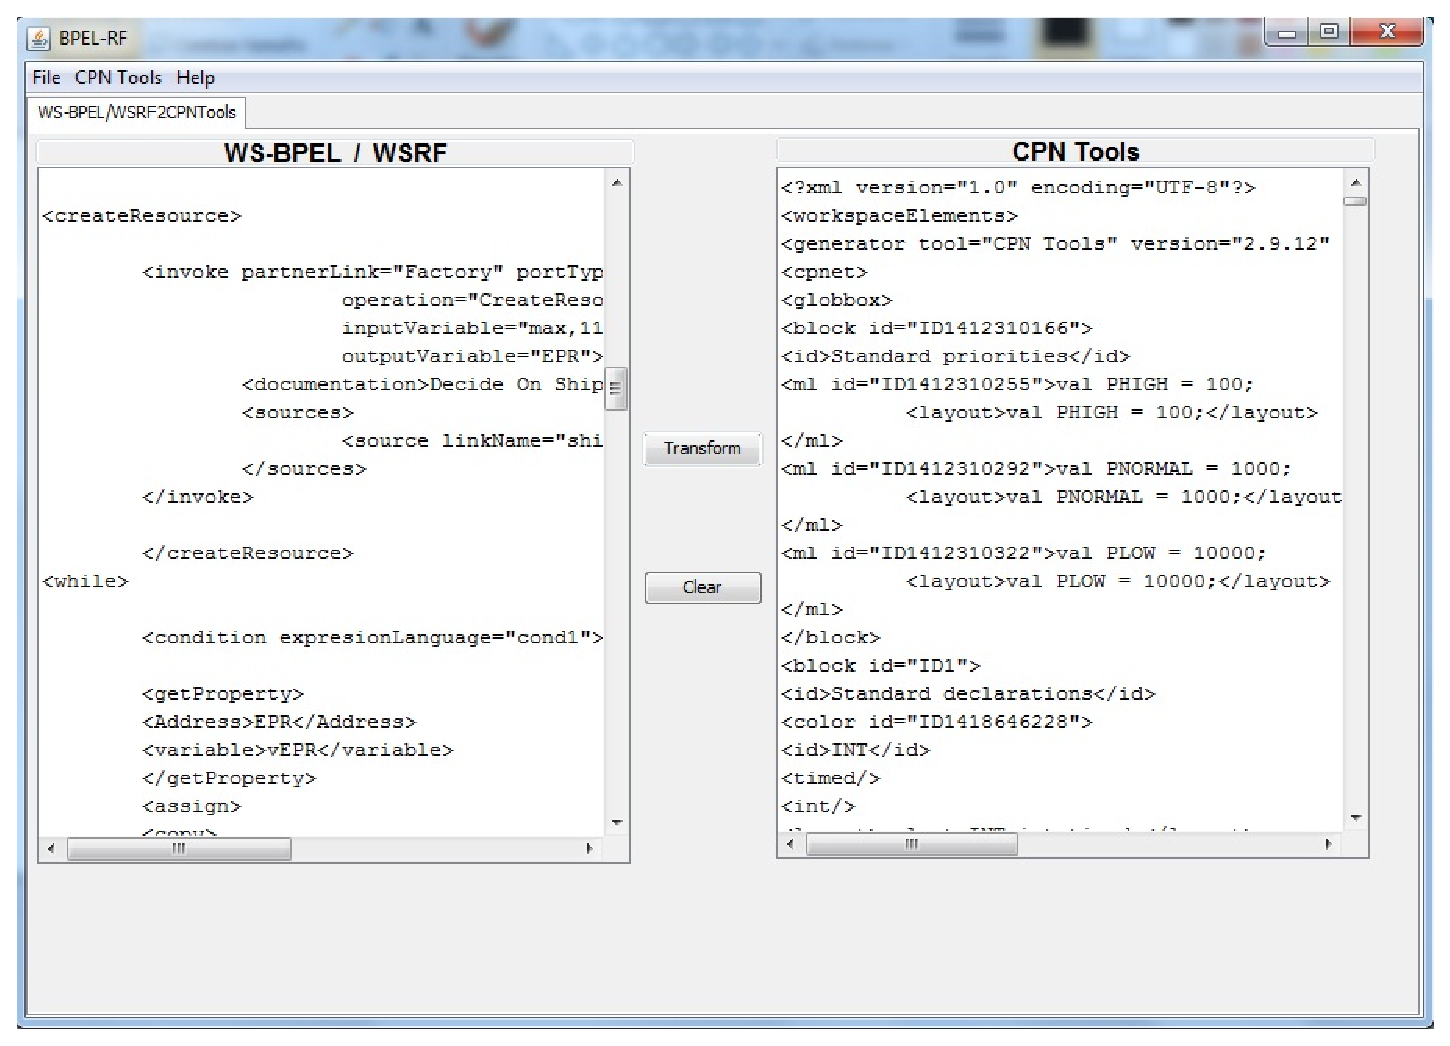
\includegraphics[width=\columnwidth,height=7cm]{Figures/mainscreen.eps}
\vspace{-0.8cm} 
\caption{Main screen of the tool.}
\label{main}
\end{figure}
\end{center}
\vspace{-0.5cm} 
%Thus, the user only needs to click on the appropriate tab in order to perform a specific %translation. Thus, we now have a new tab, called ``WS-CDL2CPNTools'', which is used to %transform the WS-CDL specification into a PTCPN. Figure \ref{WSTTools} shows a picture of %the WST Tool and the transformation from a WS-CDL document to a PTCPN.\\
The main elements of the interface are:
\begin{itemize}
\item{The \textbf{WS-BPEL / WSRF Textbox} permits users to introduce
XML code following the specification given by WS-BPEL and WSRF. This XML is
used as the source code to be translated into PTCPN.
This code can be introduced in two ways; either by writing the XML code by hand or
by loading a previously saved document using the \emph{Open WS-BPEL WSRF File} submenu mentioned above. A dialog window will be shown to the user asking him to select the document to be opened. If the file is not valid, an error message will be displayed on the screen.}

\item{In the \textbf{CPNTools Textbox}, after clicking on the button ``Transform'',
the corresponding Petri Net XML specification is shown. To save this specification, the user must click on the \emph{Save Colored Petri Net File} option in the CPN Tools menu. A dialog window will be shown to the user to choose the destination folder.}
\end{itemize}

Moreover, we have another two buttons on the screen:

\begin{itemize}
\item{\textbf{The Transform button}
generates the corresponding PTCPN. The result will be automatically displayed in the CPN Tools Textbox after a few seconds. If the WS-BPEL WSRF Textbox is empty, pressing the Transform button will have no effect.}

\item{\textbf{The Clear button}
is used to clean the contents of both text boxes. If both are empty, pressing on this button will have no effect.}
\end{itemize}

{\bf Comentario para Valent\'in: Tengo los dos casos de estudio que vienen a continuaci\'on. Uno es m\'as complejo, pero no incluye un an\'alisis en CPNTools detallado, mientras que el otro es m\'as sencillo, pero tiene un an\'alisis detallado en CPNTools. Puedo dejar los dos aunque son muy parecidos. Si dejamos solo uno, cu\'al dejar\'ias?}
\section*{Case study: Online auction service}\label{cs}

The case study concerns a typical online auction process, which consists of three participants:
the online auction system and two buyers, A$_1$ and A$_2$. A seller owes a good that wants to sell to the highest possible price. Therefore, he introduces the product
in an auction system for a certain time. Then, buyers (or bidders) may place bids for the product and, when time runs out, the highest bid wins. In our case, we suppose the resource is the product for auction, the value of the resource property is the current price (only the auction system can modify it), the resource subscribers will be the buyers, their subscription conditions hold when the current product value is higher than their bid, and the resource lifetime will be the time in which the auction is active. Finally, when the lifetime has expired, the auction system sends a notification to the buyers with the result of the process (the identifier of the winner, $v_w$) and, after that, all the processes finish. Let us consider the choreography ${\it C=(O_{sys},O_1,O_2)}$, where 
${\it O_i=(PL_i,Var_i,A_i,A_{f{_i}},\mathcal{A}_{e{_i}})}$,~i=1,2,~${\it Var_{sys}=\{v_w,v_1,v_2,v_{EPR},}$
${\it at,t\}}$,~${\it Var_1= }$ \\ ${\it \{at_1,v_1,v_{w{_1}}\},\ Var_2=\{at_2,v_2,v_{w_{2}}\},\ A_{f{_1}}=exit,}$ and
${\it A_{f{_2}}=exit}$. Variable $v_{EPR}$ serves to temporarily store the value of the resource property before being sent; $v_1$, $v_2$, $v_{w_{}}$, $v_{w_{1}}$, $v_{w_{2}}$ are variables used for the interaction among participants, and, finally, $at$, $at_1$ and $at_2$ are used to control the period of time in which the auction is active. In this example, we consider a period of 10 time units. Suppose ${\it s_{0{_{sys}}}, s_{0{_1}}}$ and ${\it s_{0{_2}}}$ are the initial states of $O_{sys}$, $O_1$ and $O_2$, respectively, and all the variables are initially $0$: \\[-0.2cm]


\noindent 
%
${\it A_{sys}=assign(10,at);
			createResource(EPR,25,11,A_{not});
			}$ \\\indent \hspace{0.6cm} ${\it
			while(actualTime()<=at,A_{bid})}$\\
%
${\it A_1=wait(1,1);
		subscribe(O_1,EPR,EPR>=0,A_{cond_{1}});
		}$ \\\indent \hspace{0.6cm} ${\it
		invoke(pl1,auction\_time_1,at1); 
		\overline{reply}(pl1,auction\_time_1,at1);
		}$ \\\indent \hspace{0.6cm} ${\it
		while(actualTime()<=at1,A_{bid_{1}})};
		receive(pl3,bid\_finish_1,vw_1,empty)$\\
%
${\it A_2=wait(1,1);
		subscribe(O_2,EPR,EPR>=0,A_{cond_{2}});
		}$ \\\indent \hspace{0.6cm} ${\it
		invoke(pl2,auction\_time_2,at2);\\ 
		\overline{reply}(pl2,auction\_time_2,at2);
		}$ \\\indent \hspace{0.6cm} ${\it
		while(actualTime()<=at2,A_{bid_{2}})};
		receive(pl4,bid\_finish_2,vw_2,empty)$\\ 
%being:\\
%
${\it A_{not}= %while(v_{EPR}==v1,assign(1,vw));
		%while(v_{EPR}==v2,assign(2,vw));
		%}$ \\\indent \hspace{0.6cm} ${\it
		((invoke(pl_3,bid\_finish_1,v_w)||
		invoke(pl_4,bid\_finish_2,v_w))}$\\
%
${\it A_{bid}= getprop(EPR,v_{EPR}); 
		pick(
			}$ \\\indent \hspace{0.6cm} ${\it
			(pl1,auction\_time1,t,reply(pl1,auction\_time1,at)),
			}$ \\\indent \hspace{0.6cm} ${\it
			(pl2,auction\_time2,t,reply(pl2,auction\_time2,at)),
			}$ \\\indent \hspace{0.6cm} ${\it
			(pl_1,cmp,v_1,while(v_1>v_{EPR},assign(v1,v_{EPR});
			}$ \\\indent \indent \hspace{0.6cm} ${\it
			setProp(EPR,v_{EPR});assign(1,vw))),
			}$ \\\indent \hspace{0.6cm} ${\it
			(pl_2,cmp,v_2,while(v_2>v_{EPR},assign(v2,v_{EPR});
			}$ \\\indent \indent \hspace{0.6cm}${\it 
			setProp(EPR,v_{EPR});assign(2,vw))),empty,1)}$\\
% 
${\it A_{cond_{1}}=getProp(EPR,v_{EPR});
		invoke(pl_1,{bid\_up}_1,v_{EPR})}$\\
%
${\it A_{cond_{2}}=getProp(EPR,v_{EPR});
		invoke(pl_2,{bid\_up}_2,v_{EPR})}$\\
%
${\it A_{bid_{1}}= receive(pl_1,bid\_up_1,v_1);
		assign(v_1+random(),v_1);
		}$ \\\indent \hspace{0.55cm} ${\it
		invoke(pl_1,cmp,v_1);
		subscribe(O_1,EPR,EPR>v_1,A_{cond_{1}});
		wait(1,1)}$\\
%
${\it A_{bid_{2}}= receive(pl_2,bid\_up_2,v_2);
		assign(v_2+random(),v_2);
		}$ \\\indent \hspace{0.55cm} ${\it
		invoke(pl_2,cmp,v_2);
		subscribe(O_2,EPR,EPR>v_2,A_{cond_{2}});
		wait(1,1)}$\\
\\
Regarding to the operations $auction\_time1$ and $auction\_time2$ inform buyers about the period of time in which the auction is active via variables $at$, $at1$ and $at2$, which are used in the while structures to control this period. The operations $bid\_up_{1}$ and $bid\_up_{2}$ are used to increase the current bid by adding a random amount to the corresponding variable $v_i$. The operation $cmp$ is an auction system operation that receives as parameter a variable of the buyers, $v_i$. If the value of this variable is greater than the current value of $v_{EPR}$, then $v_{EPR}$ is modified with this new value, that is, the new bid exceeds the current bid. After that, by means of the activity $setProp(EPR,v_{EPR})$, we can update the value of the resource property with the new bid. Finally, the operations $bid\_finish_{1}$, $bid\_finish_{2}$ update the value of $v_w$ to inform the buyers who is the winner once the auction has expired. 


In Fig.~\ref{casestudy}, we depict a simplified version of the PTCPN for the online auction system. The complete model can be accessed at the following web address: \url{http://www.dsi.uclm.es/retics/bpelrf/}. Here, we have constructed a hierarchical net relying on the notions of substitution transitions, sockets and ports offered by CPNTools~\cite{Jensen2009}. 
%Each substitution represents the PTCPN of the corresponding activity following the models presented in previous sections.
%As well, each orchestrator have its own exit and error places as well as its correct output places so that an error or an exit activity invocation only affects to the corresponding orchestrator allowing to the others orchestrators to continue their workflow without being interfered. %Finally, for the sake of clarity, we have reused the variables places for all participants despite each one has its own variables places.    
%Valent’n indica:
We have then simulated and analysed the system, and we have concluded that the system finalizes successfully, that is, the output place of the system ($p\_ok$) is reached in all the simulations. To check the consistency of the model, we have simulated the possibility of reaching an error place. For instance, if we delete the $wait(1,1)$ sentences from activities $A_1$ and $A_2$, then it would imply that the buyers could access to the resource, that is the bid, even before the resource has been created. This possibility would trigger the expected error. Furthermore, we have analysed the data output from an experiment consisting of 5000 simulations. From the analysis of these data, we observe that the system is fair, from the point of view of the buyers, since they have equal right to place a bid. Indeed, the average of placed bids from each buyer is similar. Other information gathered from these data shows that buyers can evenly place higher bids than their competitors. %Another experiment with 5000 simulations that considers removing the wait sentences shows us that the percentage of reaching $p\_ok$ is 23\% in opposite to a percentage of 77\% of reaching an error state.

\begin{figure}[!ht]
\begin{center}
\fbox{\parbox[t]{10cm}{\begin{center}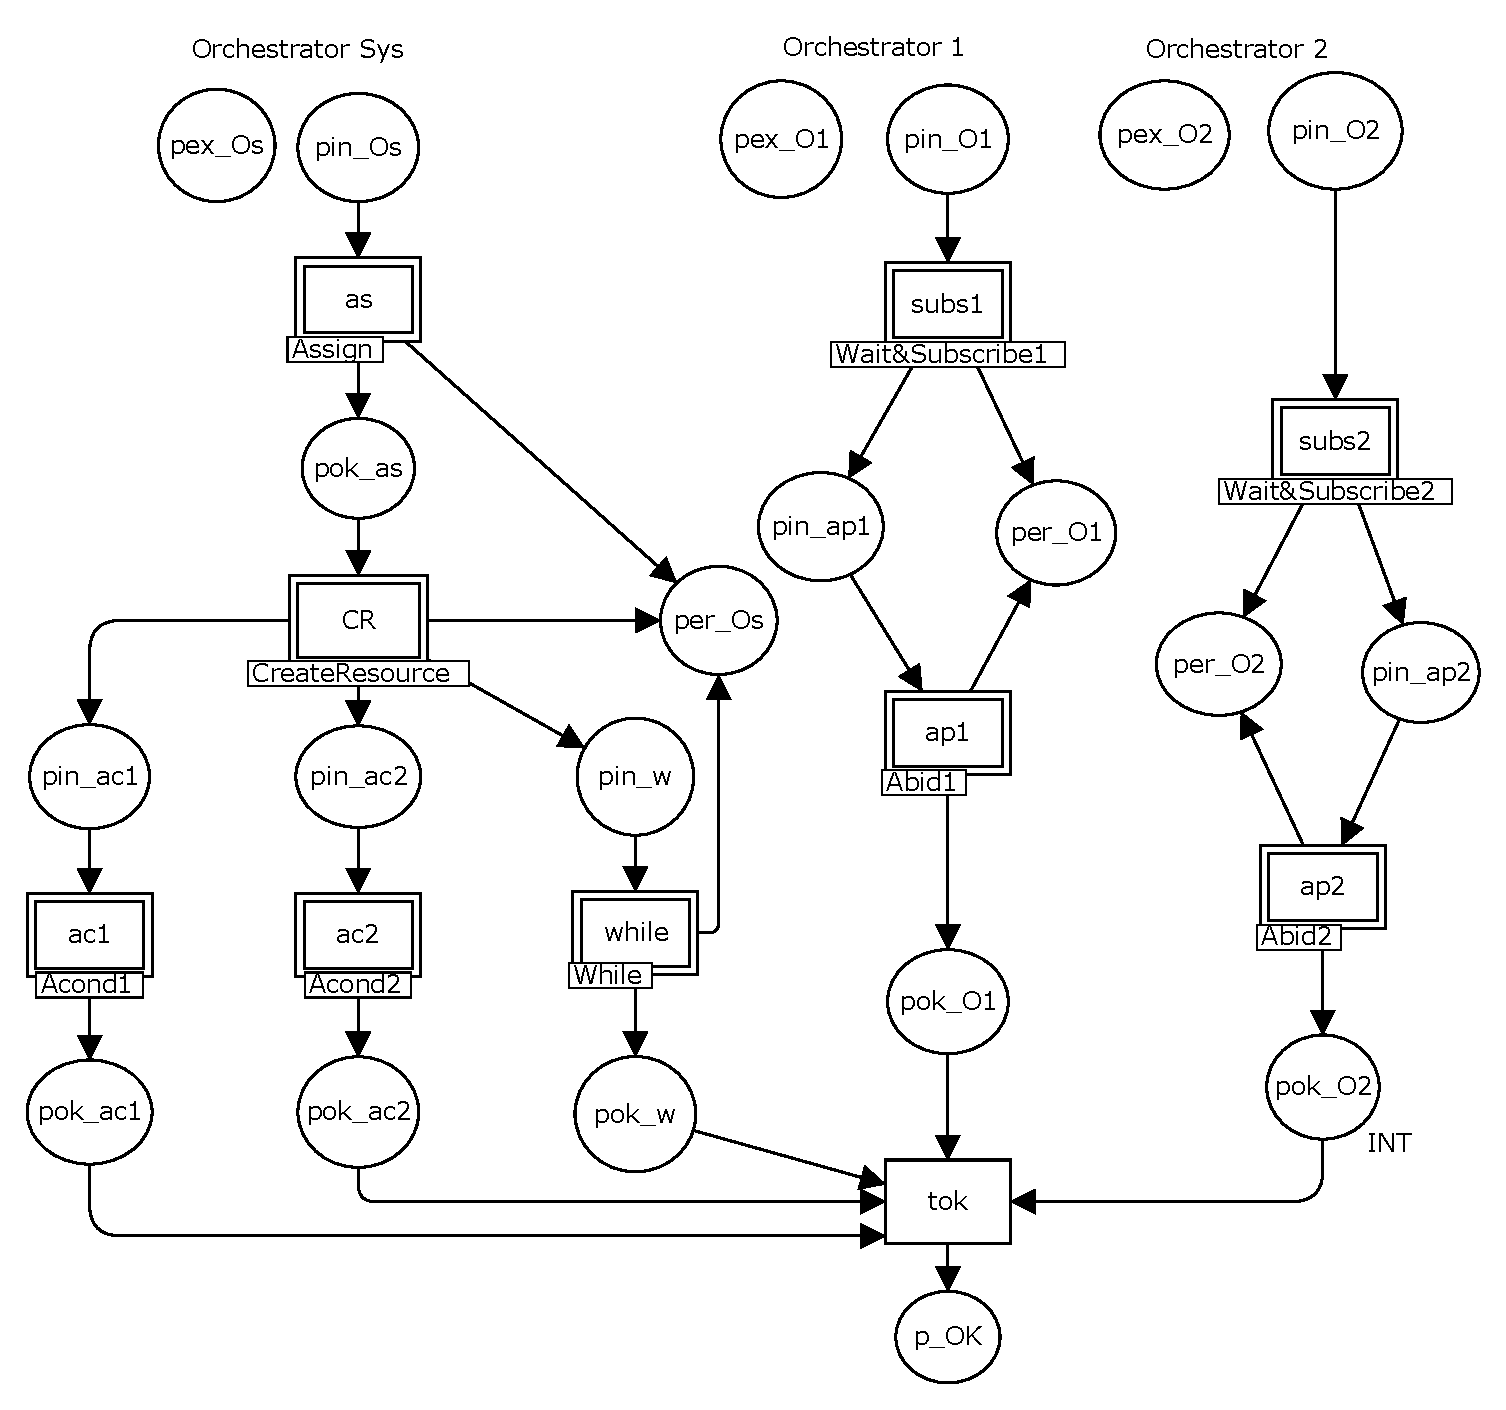
\includegraphics[scale=0.35]
{Figures/casestudy.eps}\end{center}}}
\end{center}
\vspace{-0.6cm}
\caption{\label{casestudy} A simplified PTCPN for the online auction system.}
\end{figure}

\section{Case Study 2}
The case study concerns a typical automatic management system for stock market investments, which consists of {\em n+1} participants:
the online stock market system and {\em n} investors, A$_i$, $i=1,\ldots, n$. Here, the resource will be the stocks of a company that the investors want to buy just in case the price falls below an established limit, which the investors fix previously by means of subscriptions, i.e., an investor subscribes to the resource (the stocks) with a certain guard (the value of the stocks he/she want to pay for it). The lifetime {\em lft} will be determined by the stock market system and the resource price will be fluctuating to simulate the rises/drops of the stock. Notice that we do not take into account the stock buy process since our aim is to model an investors' information system. Thus, the participants will be notified when their bids hold or the resource lifetime expires.  
Let us consider the choreography ${\it C=(O_{sys},O_1,\ldots,O_n)}$, where 
\mbox{${\it O_k=(PL_k,Var_k,A_k,A_{f{_k}},\mathcal{A}_{e{_k}})}$,~k=sys,~1,...,~n;}~\mbox{${\it Var_{sys}=}$} \\${\it \{at,vEPR\}, Var_i= \{v_i\},\ A_{f{_k}}=}$  ${\it exit}$. Variable $v{EPR}$ serves to temporarily store the value of the resource property before being sent; $v_i$ is the variable used for the interaction among participants, and, finally, $at$ controls the period of time in which the auction is active. Note that the value {\em x} indicates the resource value at the beginning, {\em at0} is the time that the ``auction'' is active, and, finally, {\em $x_i$} is the value of the stocks that he/she wants to pay for. Suppose that all the variables are initially $0$: 
%\vspace{-0.3cm}
\begin{flushleft}
\small{ 
${\it Asys=assign(x+1,vEPR);assign(at0,at);}$\\
$\hspace{1cm}{\it  CreateResource(EPR,lft,x,empty);}$\\	
$\hspace{1cm}{\it  while(actualTime()<=at,Abid)}$\\
${\it Abid=getProp(EPR,vEPR);assign(vEPR+bid(),vEPR);}$\\	
\hspace{1cm}${\it setProp(EPR,vEPR);wait(1,2)}$\\
${\it A_i=wait(1,2);subscribe(O_i,EPR,EPR<x_i,Acond_i);}$\\
\hspace{0.8cm}${\it pick((pl_i,buy,v_i,empty),empty,at0)}$\\
${\it Acond_i=getProp(EPR,vEPR);invoke(pl_i,buy,vEPR)}$\\
}
\end{flushleft}

Here, the function {\it bid} is used to increase/decrease the stocks value simulating the fluctuation of the stocks price.

\begin{figure}[h]
%\fbox{
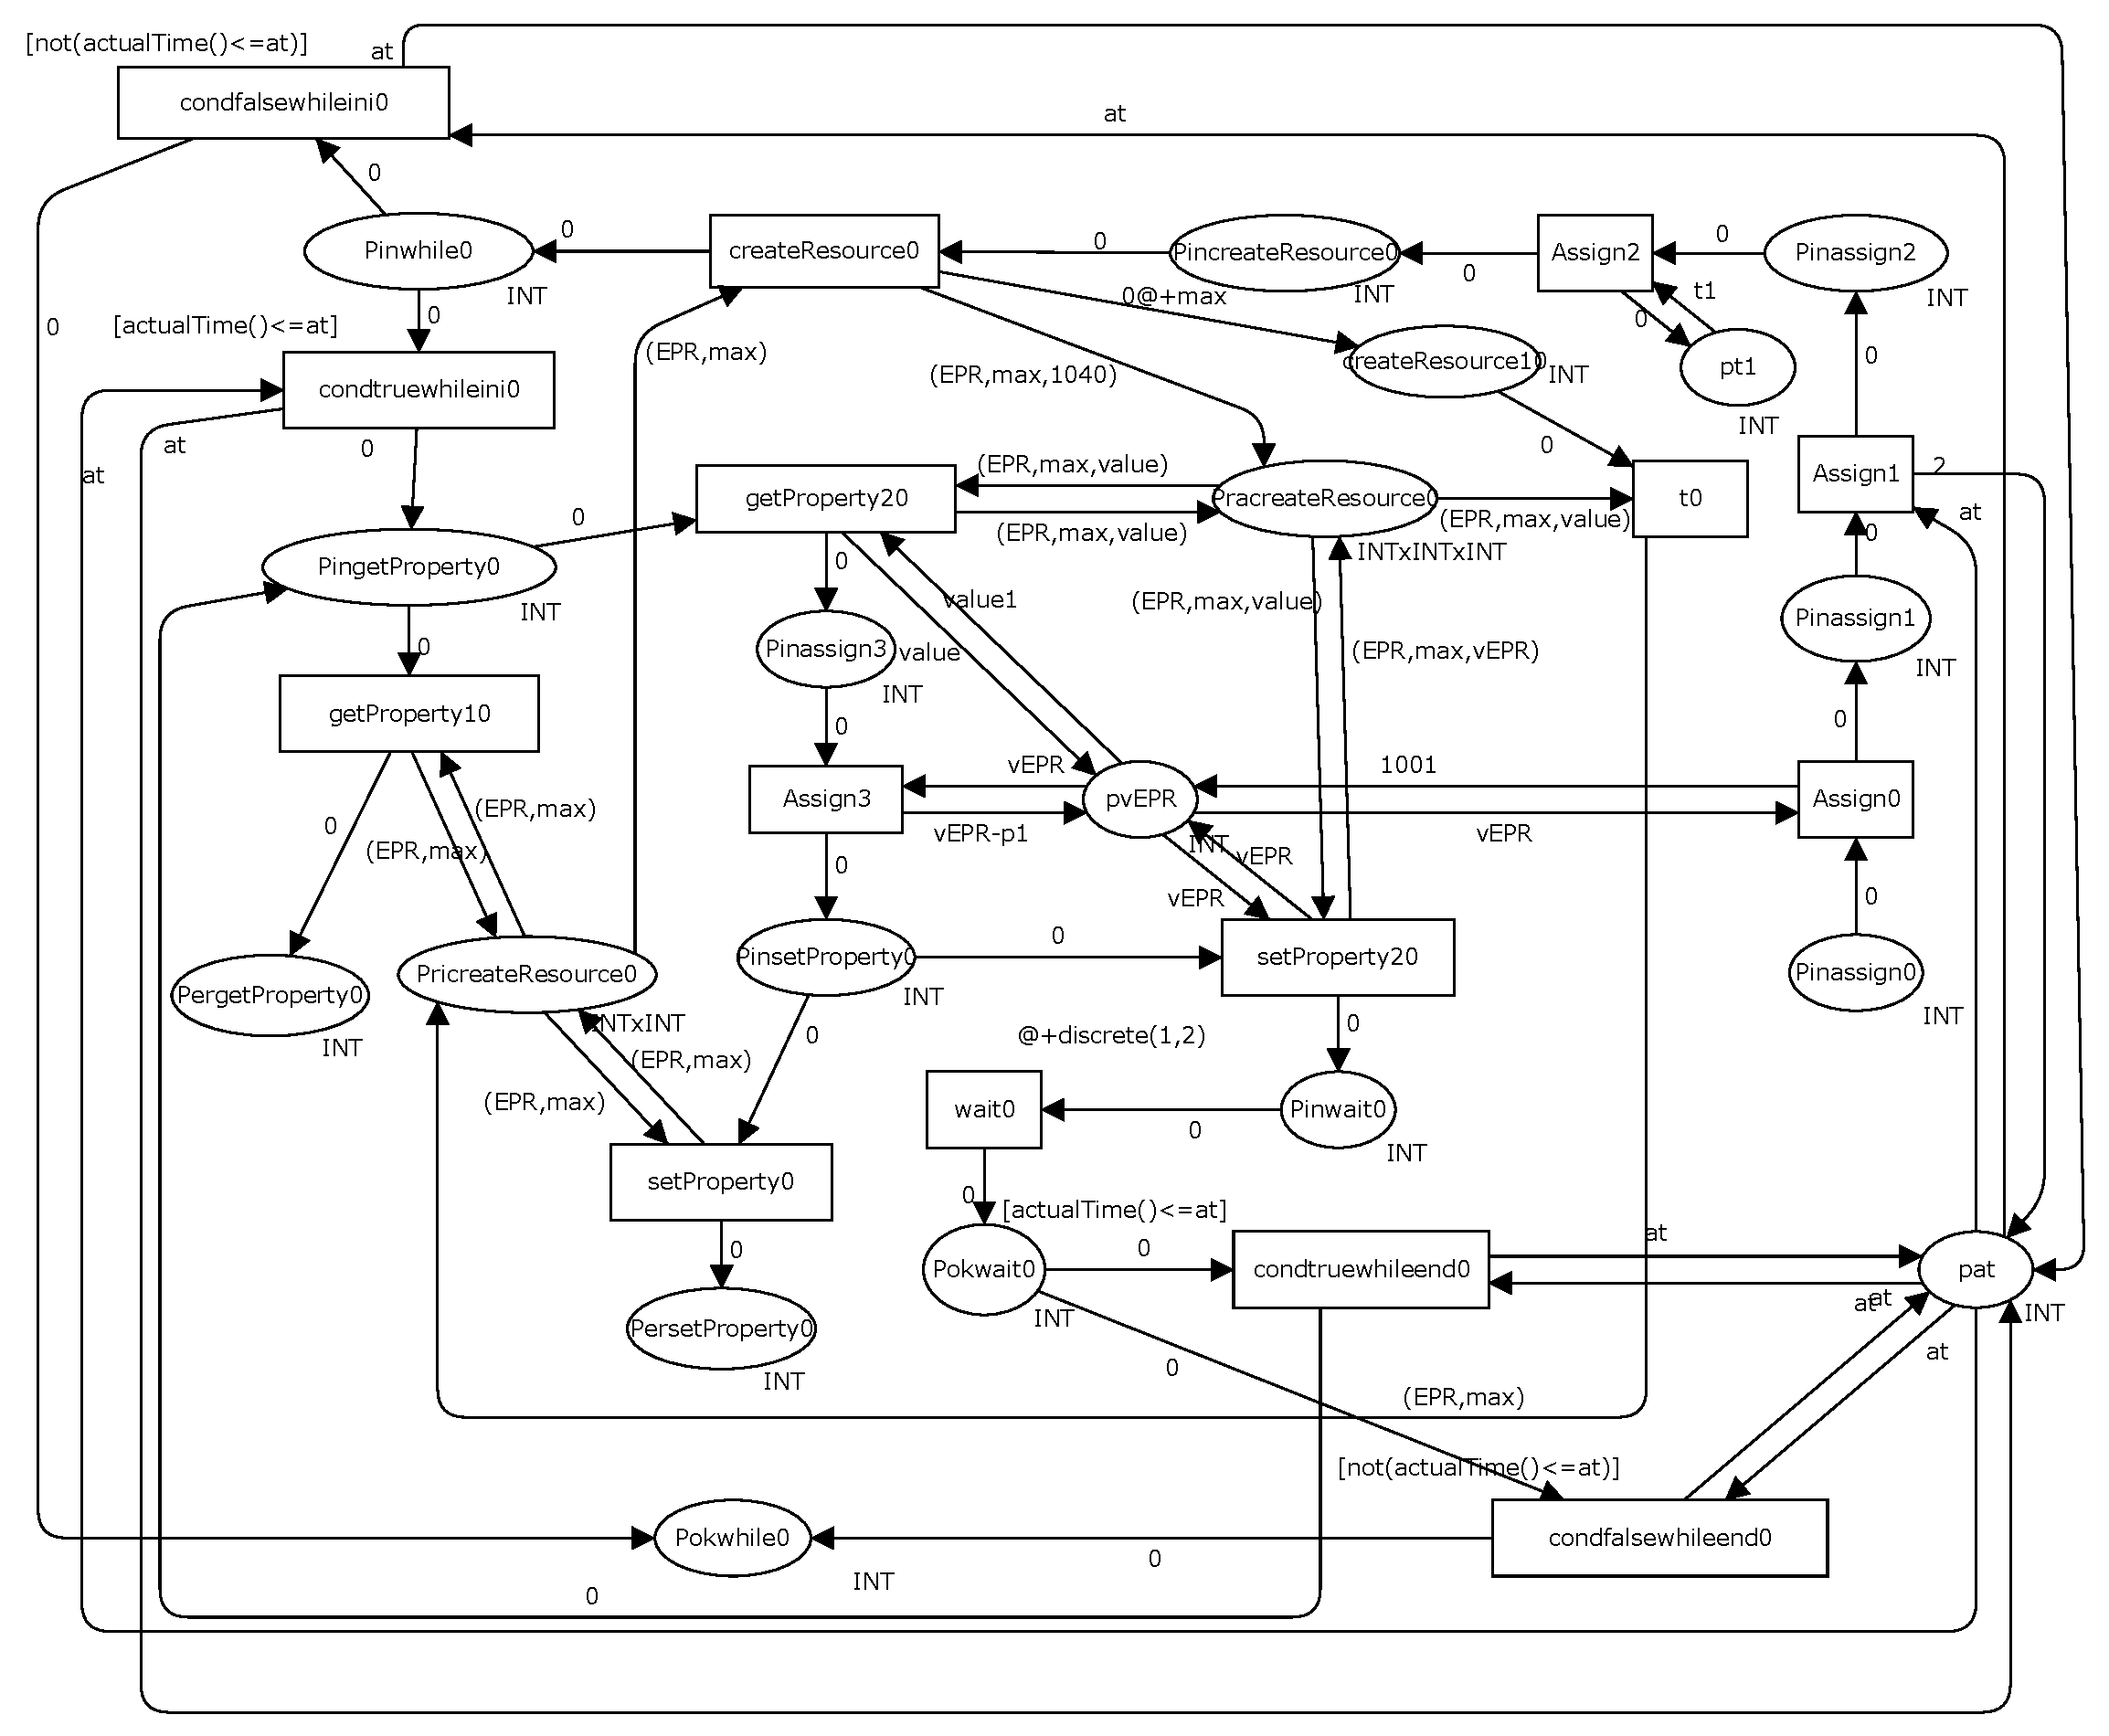
\includegraphics[width=\columnwidth, height=10cm]{Figures/sistema.eps}
\vspace{-0.6cm}
\caption{PTCPN of the online stock market.}\label{sistema}
\end{figure}
In Figs. \ref{sistema} and \ref{proceso}, the PTCPNs for one buyer and for the system are depicted.  These figures have been obtained automatically by using our tool. 
\begin{figure}[h]
%\fbox{
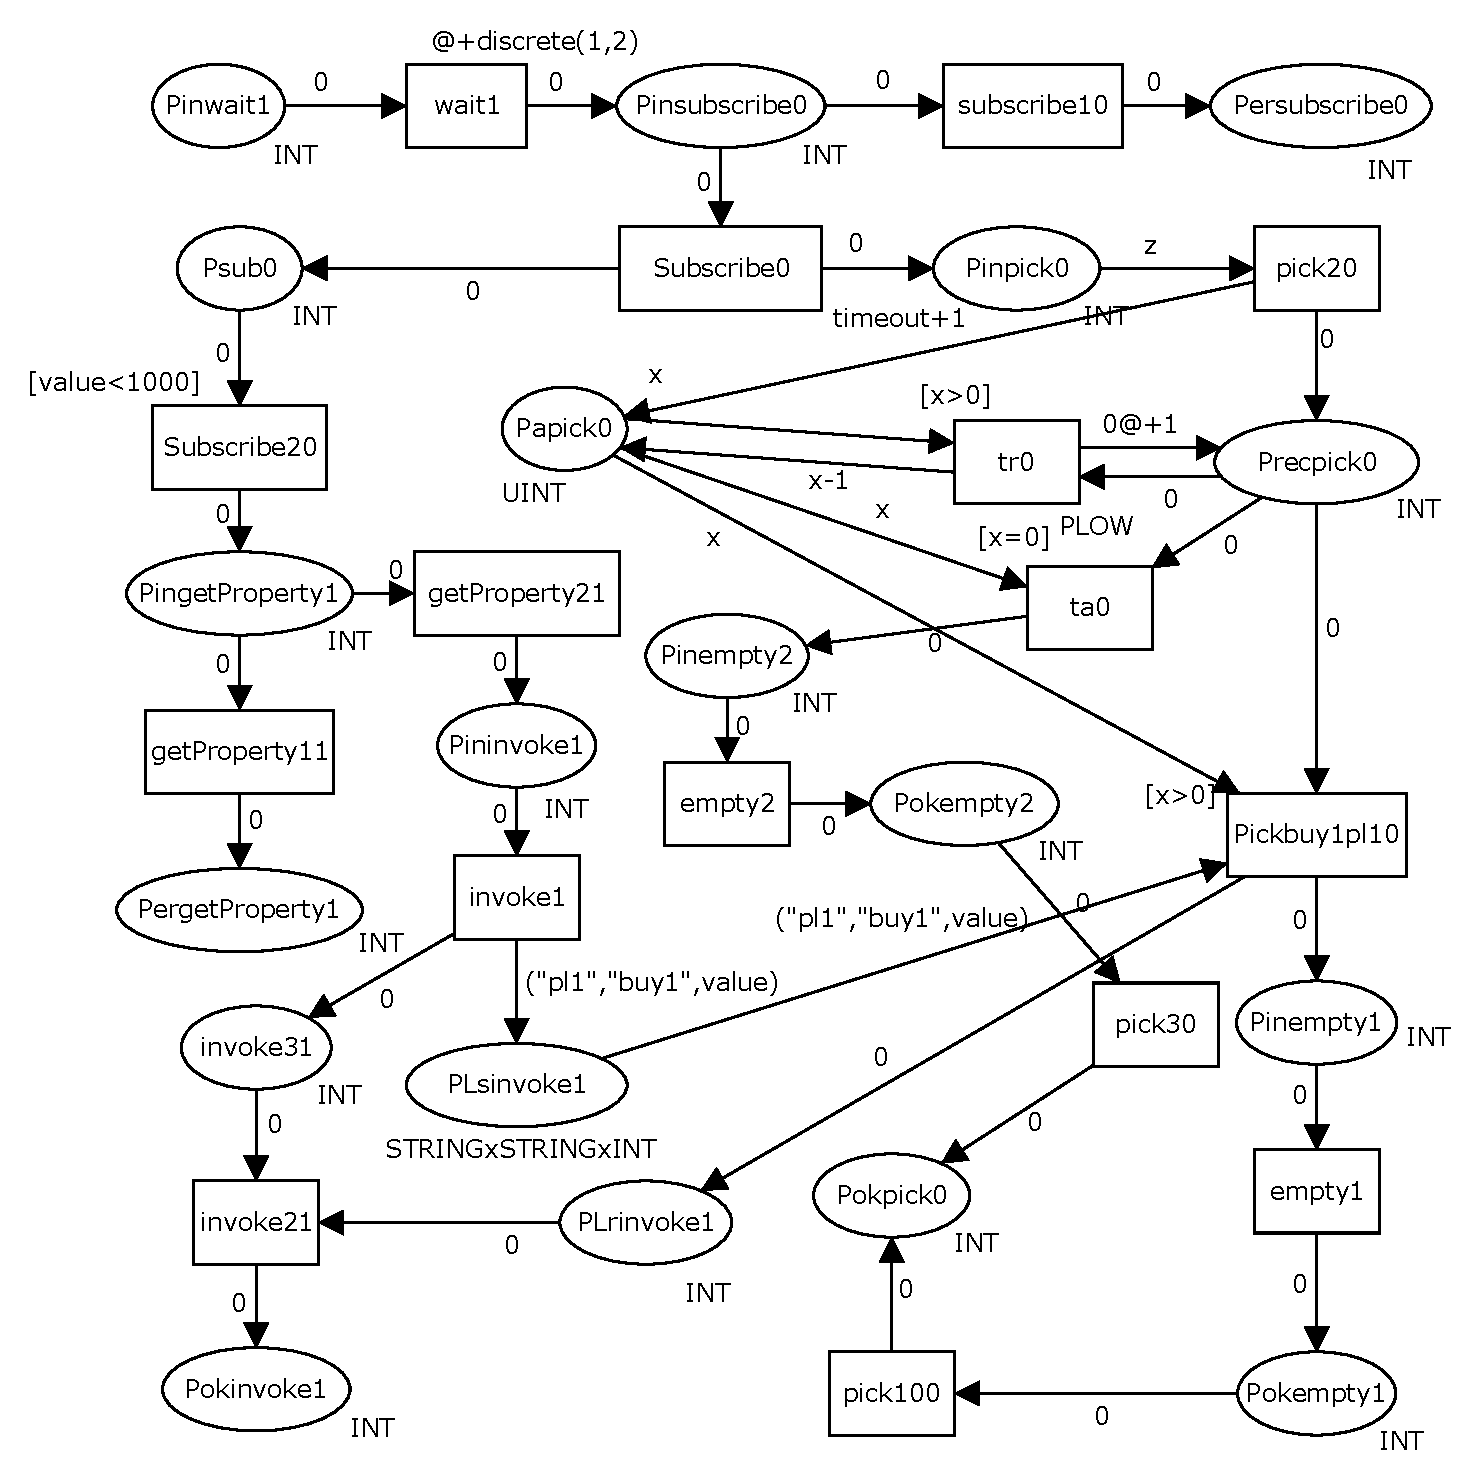
\includegraphics[width=\columnwidth, height=10cm]{Figures/proceso.eps}
\vspace{-0.8cm}
\caption{PTCPN of one buyer.}\label{proceso}
\end{figure}

\subsection{Analysis}\label{analysis}
CPNTools offers us two forms to check the correctness of our system: formal verification and simulation. 
First, the simulation helps designers to understand how the system exactly works and it is a mean to
detect possible errors in early stages of the development process in order to refine the model according the
clients' requirements. Besides, formal verification through state space
analysis could be done in order to ensure that our system achieves some formal properties such as liveness, deadlock-freeness and so on.
In this way, Table \ref{state_space} shows the
results obtained considering 1, 2, 3, 4 or 5 investors. Note that we have considered the following assumptions:

\begin{itemize}
 \item The ``auction'' time {\em at0} is limited to 10 time units.
 \item The resource is active during 15 time units ({\em lft=15}).
 \item The resource value {\em x} is 100 money units.
 \item The value of subscription of each investor {\em i}, {\em $x_i$}, is $x-(9+i)$, that is, if the system has only one investor its subscription guard will be $x<90$, whereas with 5 investors, the last investor will have a subscription guard of $x<86$.
 \item The function {\it bid} will fluctuate the stocks price between -2 and 1 in order to simulate that the price only can rise 1 and drop 2 at most each time unit. 
\end{itemize}
We will focus on deadlock-freeness to ensure that the
system never gets stuck while the participants have activities to do
in their workflow. We have leveraged the functions offered by CPNTools
to demonstrate that in all dead markings of the system the final
place is marked, which leads us to conclude the system has finished
correctly. This final place, {\em Pokfinal0}, is marked by a transition when all the participants have finished their workflow. For the sake of clarity, we have not drawn this place in each figure. Thus, the next SML code checks when this situation
occurs:\ \mbox{{\small{fun DesiredTerminal n =((Mark.PetriNet'Pokfinal0
1 n) ==
1'true)}}}, \\
which returns {\em true} if the place {\it Pokfinal0} is marked. In
addition, it is needed to evaluate the following predicate:
\mbox{{\small{  PredAllNodes
DesiredTerminal=ListDeadMarkings()}}}, to check \\that the list of
dead marking contains the marking of the {\em Pokfinal0} place.

\begin{table} [htp]
\centering
\footnotesize{
\begin{tabular}{|c|c|c|c|c|c|}
  \hline
  % after \\: \hline or \cline{col1-col2} \cline{col3-col4} ...
     & \multicolumn{5}{c|}{Number of investors}\\\cline{2-6}%\hline
  Properties     & 1 & 2 & 3 & 4 & 5 \\ \hline
  State Space Nodes & 3561  & 7569 & 16983 & 50350 & 89879 \\
  State Space Arcs & 5203 & 12843 & 33271  & 112101 &262215 \\
  Time (s) & 2 & 7 & 23 & 146 &  1140\\
  Dead Markings & 124 & 244  & 454  & 1108 &  874 \\
  \hline
\end{tabular}
}
\vspace{-0.2cm}
\caption{State space analysis results}
\label{state_space}
\end{table}
\vspace{-0.5cm}
In Fig. \ref{queries}, we show the results offered by CPNTools to
our queries for the case of {\bf three} investors. Here, it can be
appreciated that all dead markings hold the predicate {\em DesiredTerminal}, and, therefore, when the system reaches a dead marking is because system has terminated, which demonstrates the absence of deadlocks in our case study. 
%On the contrary, in Fig. \ref{RG} we can see a part of the reachability
%graph from the initial marking to a dead marking. This trace can be used for the designer to follow the path from the initial marking to the final marking in order to inspect if the system behaves according to its specification.

%In this subsection, we are going to show the experiments conducted for the case study. CPNTools offers two ways
%to demonstrate the correctness of the system: formal verification and simulation. On the hand, the user can use
%the state space analysis tool to do formal verification
%in order to check some properties of the model such as liveness, deadlock-freeness, fairness and so on.
 %It is worthwhile to mention we will obtain more
%than one dead marking as we do not introduce in the model any
%mechanism to clean the marking of the variables, the partnerlinks,
%etc. when the final marking is reached. The solution is pretty
%straightforward, but could be a little bit tedious to draw
%transitions to reset the places when the final place is marked. As
%opposed to this, w
\begin{figure}[h]
\begin{center}%\fbox{
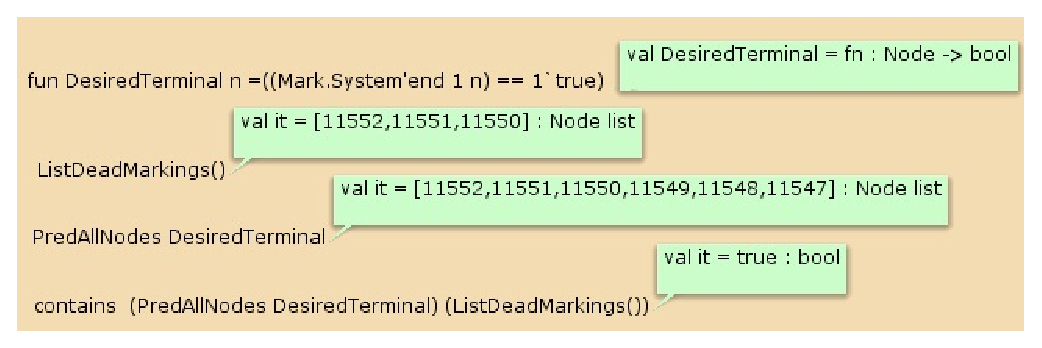
\includegraphics[width=\textwidth,height=3cm]{Figures/queries.eps}
\vspace{-0.7cm}
\caption{Result of the queries in CPNTools.}\label{queries}
\end{center}
\end{figure}
\vspace{-0.7cm}
%
%\vspace{.3cm}
%
%\begin{figure}[h]
%%\fbox{
%\includegraphics[width=\columnwidth,height=6cm]{Figures/grafomarcadoscpn.eps}
%\vspace{-0.6cm}
%\caption{Partial reachability Graph (3 investors).}\label{RG}
%\end{figure}




\section{Summary}\label{sumBPELRF}
\markright{~\ref{sumBPELRF} Summary}
In this chapter, we have integrated two complementary approaches in order to improve the definition of business processes models on BPEL by adding
the capability of storing their state. We have thus transformed {\em stateless} business processes into {\em stateful} business processes. 
First, we have presented a formal model for the description of composite Web services with resources associated, and orchestrated
by a well-know business process language (BPEL). The main contribution has therefore been the integration of WSRF, a resource management language, with BPEL, taking into
account the main structural elements of BPEL, as its basic and structured activities, notifications, event handling and fault handling. Furthermore, special attention has been given to timed constraints, as WSRF consider that resources can only exist for a certain time (lifetime). Thus, resource leasing is considered in this work, which is a concept that has become increasingly popular in the field of distributed systems. To deal with notifications, event handling and fault handling, the operational semantics has been defined at three levels, the outermost one corresponding to the choreographic view of the composite Web services.


Second, we have defined a prioritised-timed coloured Petri net model and presented its corresponding semantics to represent the constructions of WS-BPEL and the standard selected for the definition of resources, namely WSRF. Apart from including the notion of state in business processes, our work also includes a publish-subscribe notification system based on WS-BaseNotification, presenting a TCPN model and its semantics. Thus, an orchestrator can show interest of being notified when a condition holds, e.g, the load of a server exceeds a certain limit. Our approach is based on the one used in CPNTools, allowing us to take advantage of its capability of analysis and verification systems. Moreover, our work in progress is the development of a tool\footnote{The beta version can be accessed at: \url{http://www.dsi.uclm.es/retics/bpelrf/}} to transform automatically WS-BPEL and WSRF specifications into CPNTools nets. As future work, we plan to study some interesting properties such as safeness, soundness and so on. As well, it is interesting to define a complete semantics of WS-BPEL and WSRF. Finally, as commented above, we defined an operational semantics in a previous work, so we will demonstrate in a future work the equivalence between both semantics.

